\documentclass[10pt,letterpaper]{article}
\usepackage[margin=1.25in]{geometry}
\usepackage[utf8]{inputenc}
\usepackage{amsmath}
\usepackage{amsfonts}
\usepackage{amssymb}


%% Sets page size and margins
\usepackage{tikz}
\usepackage{asymptote}
%\usepackage{achicago}

%% Useful packages
%\usepackage{amsmath}
\usepackage{graphicx}
\usepackage{subfig} % Package for subfigures
\usepackage[countmax]{subfloat}  %For text beneath subfigures
% To place mutlipe images
% https://tex.stackexchange.com/questions/84889/combining-multiple-eps-files-into-a-single-figure
\usepackage[colorinlistoftodos]{todonotes}
\usepackage[colorlinks=true, allcolors=blue]{hyperref} 
\usepackage{caption} % Package for captions
\usepackage{soul} % to wrap underlined sentences
\usepackage{float} %package for floats
%\floatstyle{boxed} % For figure with boarders + next line
%\restylefloat{figure} % For figure with boarders + above line
%\usepackage{dcolumn} % For Sideways tables
\usepackage{rotating} % Rotate table


% kableExtra packages
\usepackage{booktabs}
\usepackage{longtable}
\usepackage{array}
\usepackage{multirow}
%\usepackage[table]{xcolor}
\usepackage{wrapfig}
\usepackage{float}
\usepackage{colortbl}
\usepackage{pdflscape}
\usepackage{tabu}
\usepackage{threeparttable}
\usepackage{threeparttablex}
\usepackage[normalem]{ulem}
\usepackage{makecell}

\interfootnotelinepenalty=10000 % Makes footnotes appear on the same page

%% Citations and References
\usepackage{natbib}
\bibliographystyle{chicago}
\setcitestyle{authoryear,open={(},close={)}}
\usepackage{setspace}
\onehalfspacing



% First Page Details
\author{David Simpson\footnote{David Simpson (dcs2171@columbia.edu): Doctoral Student, Department of Political Science, Columbia University, 420 West 118th Street, New York, NY 10027. Special thanks to Jeffrey Lax for his helpful comments, time, and advice on this project.}}

\title{Proposal: Hide and Seek Representation: \\ 
\large Signaled vs Revealed Responsiveness in the 106th House}

\begin{document}
\maketitle

\begin{abstract}
This paper considers the relationship between constituency preferences and legislator roll-call behavior. Results demonstrate that responsiveness measures are sensitive to the classification of independent voters. Classifying independent voters as non-same party voters rather than as independent voters masks the true responsiveness relationship between legislators and sub-district level constituent groups. This paper also explores other the sensitivity of other ideology measures.
\end{abstract}

%%%%%%%%%%%%%%%%%%%%%
%\begin{} Introduction Section
%%%%%%%%%%%%%%%%%%%%%
\section{Introduction/Proposal}
What is the relationship between voter preferences, legislator behavior, and policy outcomes? Answering such a question is essential to assessing the health of representative democracy in the United States. The goal of this paper is to contribute to the field's assessment of US representation and responsiveness through three contributions. First, this paper resolves a representation puzzle identified in \cite{Clinton2006}. The puzzle suggests that Republican legislators in the 106th House of Representatives were responsive to same-party district constituents where as Democratic legislators were responsive to only non-same-party constituents. However, this observations is due to a coding error. In contrast, I find that legislators of both parties are responsive to same-party constituents. Same-party responsiveness occurs through two channels - same-party share of district constituents and same-party ideology. I also find that the nature of same-party responsiveness is conditional on vote significance. I then use the Clinton data to make two additional contributions.

Second, this paper illustrates the problem created when one lumps independent voters together with opposite party voters to measure responsiveness to non-same-party constituents. Independent lumping conceals a key and important interaction between legislators and independent voters by assuming that legislators respond uniformly to the ideology and constituent percentage share of independent voters and opposite-party voters. I find that when independents are disaggregated from opposite party voters, legislators are strongly responsive to the share and ideology of independent voters. Such a finding should make sense in context of legislator electoral competition. The average share of same-party constituents in Republican held districts is 0.39. In Democratic districts, the average share of same-party constituents is 0.45. The standard deviation of same-party shares in Democratic held districts is nearly twice that of Republican held districts. It is reasonable to expect that legislators are distinctly responsive to independent constituents since a significant number of districts do not have same-party shares larger than 50 percent.

Lastly, this paper provides new and novel evidence of what I (tentatively) call signaled vs revealed responsiveness.\footnote{I want to do more sensitivity and robustness checks, complete a wider review of the literature, and consider additional years of data to confirm that this finding is unique and not epiphenomenal. Another more catchy name for this phenomenon could be Hide and Seek representation.} I find that legislator ideology as measured by an index of all House votes is substantively different than legislator ideology as measured by an index of only key House votes. Notably, I find that the ideology score of nearly all Democratic legislators is more liberal when the score is calculated using key votes rather than all votes. Republicans; however, have a less uniform ideology change. Rather, the caucus is split. When key votes are used some Republican legislators appear more liberal and others appear more conservative. The different ideology scores is not trivial. Rather, the observed nature of legislator responsiveness to sub-district group ideology changes considerably. \textbf{Under key votes, legislators are more responsive to XYZ.}

My findings suggest that legislators may use the set of all votes to signal partisan reliability or bipartisan credibility. In contrast, the set of key votes may (1) serve as a less noisy reflection legislator ideology and (2) provide insight on how legislators optimize between satisfying same-party base voters and attracting independent voters. However, the use of vote based ideology indices is subject to some empirical problems that I discuss in this paper. It is also possible that the difference between the two ideal point measures is related to district competitiveness, the strength of political parties in the US House, and legislative bargaining with the president. I explore these possibilities; however, more analysis is needed to establish the existence and predictability of signaled vs revealed responsiveness and to disentangle the respective impact of district competitiveness, congressional party strength, and presidential bargaining power. The legislator ideology data used in this proposal is limited to legislative index scores from one chamber of one Congress (the 106th House). As such, consideration of the Senate, additional congressional sessions, and modes of assessing legislator ideology is needed to confirm whether the observed signaled vs revealed responsiveness exists across Congresses in a way is consistent and predictable. I plan to explore these various avenues for research in future drafts and papers.

\section{Literature} 
In a well functioning democracy one should expect legislator behavior to change as voter preferences change. However, understanding the responsiveness relationship between legislators and their constituents requires consideration of both the normative and positive literature on the topic. 

\textbf{Sable (2015)} argues 


same-party constituents  
As such, it is reasonable to expect 

In a health democracy, as voter preferences change, one should expect that legislator behavior changes as well.

% Normative
However, capturing the nature of this relationship has both positive and normative implications. \textbf{Theory paper} argues that legislator responsive to voter preferences is not necessarily an end (p. \#). Rather responsiveness to who and for what purpose also matters. \textbf{Minority Rights} , and \textbf{Deliberation over.} Other paper on what type of legislator. Does the % In addition to why responsiveness is important, we should wonder responsive to what? Should we expected people to always vote one way or another?

% Ineed Federalist suggests that representatives are important and deliberation is important.

Therefore, in the analysis of how responsive policy and legislators themselves are to constituents depends on the degree sits at the intersection of many questions. Who is being represented? Who is doing the representation and blah.

Empirically capturing the how fast (responsive) and how consistent (congruent) policy is provides a baseline for the positive and normative discussion. 


How are people selected? Does the person matter? Yes, people are not just conduits for. Once people are there, how does the legislative process effect their outcomes. 

% How are people selected
\textbf{How are people selected?} A natural starting place is Downs (1957). In addition to comments on the rationality of voting, Downs argued that voting in a unideminsional space with two candidates does not mirror Hotelling's model of spactial competition. Rather, the expected outcome should differ with the make up of the constituency. if voters are XYZ then candidates will compete for the center. If voters are polarized then QRS. Indeed, in the literature we find evidence of TUV. \textbf{Insert} %Need to comment on primary and general eleciton stuff

% Districitng
Similarly, recognition of this fact and public conversation regarding gerrymandering should call attention to how districting shapes who is selected. \textbf{Work on districting}

% How and What
Once legislators are in office, two questions are important. How do legislators vote - that is do the direction of their votes correspond to the preferences of their constituents, and what are they voting on?

Since, chronologically bills must make it to the floor before they are voted on and the writings of the founders both suggest the process matters - it is worth beginning there. Krehbiel argues that parties have relatively little impact in the process rather the preferences of the median voter conditional on the preferences of the veto and filibuster pivots reign supreme. Indeed a measurable test that Krehbiel (1993) offers is that we party influence should be seen through \textbf{alternative behavior}. Cameron XXXX addition of uncertainy and blah suggests that uncertainty regarding the position of pivotal legislators can help the President extract more favorable policy from Congress during legislative bargaining. Though, Howell (XXXX) suggest it is possible to see policy change outside of the bargaining process because the president can move first through unilateral actions such as executive orders. Thrower (XXX) suggests that there are limitations to this power over time.

% See that the median voter does not win
However, within the space of considered legislation there are other reasons to believe that policy outcomes do not follow the median voter. Aldrich and Rhode XXXX discuss the conditional party hypothesis, and cite the blah. Though the hypothesis is compelling, it does not seem to capture the observed strength of party leaders during periods of legislator preference heterogeneity. In contrast Cox and McCubbins argue that party leadership is not conditional. Rather, XYZ therefor we should expect QRS. Indeed they find that party control predicts the direction of legislation. Such work is relevant to historical analysis of Congressional lawmaking. \textbf{Author et al. (XXXX) describe how Southern legislators did xyz to block.} Similarly, a section of the literature focuses on who holds the legislative seat. For example, \textbf{Author (XXXX)} consider the relationship between districts and elected officials and the probability that Black representatives gain leadership positions. They find fewer Black representatives in GOP but under-representation in DEM. Due to modern districting and platform matching, it is unsurprising that less in GOP but maybe a point of concern for Democrats. \textbf{Lax and Phillips (XXXX)} find evidence of blah.

Recognizing the endogeneity of the legislative process is important. The sample of bills matters is not random.

\textbf{Other paper} argues that indeed many of the bills passed by the majority party in either chamber are used for signalling rather than blah. Such work both illustrates the type of legislation that we might expect under the Cartel Model and relates to the work on how legislator's use votes to communicate \textbf{identities} to their districts. \textbf{Author (XXXX)} described this process as legislators crafting their homestyles. \textbf{Another sentence.} \textbf{Author (XXXX)} similarly argues that there are two types of legislators XYZ and XYZ. Author argues that this contributes to increased polarization.

% Empirical aanslysis of legislative behavior
The empirical analysis of legislative behavior is extensive and has produced new methods for analysis . \textbf{Author and author} argued XYZ. Author XXXX finds. \textbf{Others find.}

Within the empirical responsiveness literature there is an active and robust conversation regarding how to measure 	

% My article
This article follows the empi literature.





Such work is consistent with paper on legislator type, and older book on homestyles.

Connect all of this to voter ideology. 


In the theoretical work on Krehbiel

In the space of positive analysis identifying 


responsiveness. It provides a baseline for ud

 researchers should consider the extent to which 

Yet a constant is that constituents choose legislators and those legislators decide policy.




Responsiveness versus congruence.




The positive approach to this question requires a continues conversation between empiricists who rigorously interrogate existing measures and methodologies. Such a rigorous debate is necessary for providing quality information during normative discussions of representation in a representative democracy. In this paper, I examine \cite{Clinton2006} which finds a responsiveness puzzle - Republican legislators are only responsive to same-party constituents where as Democratic legislators are only responsive to nonsame-party constituents. However, \cite{Clinton2006}'s models are misspecified. The primary regression models include interaction terms but fail to include the constitutive variables as separate independent variables. The replication data for the original paper is provided through Harvard Dataverse \cite{Clinton2009}. Using the original data I resolve the puzzle Clinton observes.  


Initial results resolve this puzzle by finding legislators of both parties are responsive to average district preferences as well as the preferences of both same-party and non-same party constituents. Potential future extensions include  testing whether the new findings are sensitive to other common measurement issues in the responsiveness literature such as the ``Delegate-Paradox" and the "Non-Common Scale Problem."

\section{Literature junck} 
\textbf{In the literature on responsiveness XX stands as important beginner.} \textit{Spatial model discussion.} In these frameworks, it is expected that legislators closely align to the behavior of the median voter in their district. \textbf{However, the nature of primary elections suggests that legislators may appeal to sub-district level constituency in whole, or at least during the primary.} This issue is at the forefront of the Clinton analysis. 

 \textbf{Others discuss of different ways to think about representation (forward or backward looking).} 
 
In the space of measurement there are various methods and concerns. 

Literature and relevance:
\begin{enumerate}
\item[$\bullet$] \cite{Clinton2006} - Finds that Republican (Democratic) representatives are only responsive to same-party (nonsame-party) constituents.
\item[$\bullet$] \cite{Clinton2009} - Replication Data for \cite{Clinton2006} provided through Harvard Dataverse.
\item[$\bullet$] \cite{Broockman2016} -  Shows that using roll-call votes to create legislator ideal points can cause an ideologically consistent party moderate to appear ideologically extreme (p. 182-184).
\item[$\bullet$] \cite{Ahler2018} - Describes consistency-extremity puzzle the "Delegate Paradox" and find current legislators on average better represent their constituencies than a counterfactual less polarized legislators.
\item[$\bullet$] \cite{Lax2009} - Demonstrates multilevel modeling of individual opinion and poststratification by population share (MRP) performs better than disaggregation of national surveys by state. 
\item[$\bullet$] \cite{Lax2018} - Identifies "Non-Common Scale" as the problem that arises when one attempts to compare ideology of policy to ideology of opinion when the two measures have different scales. The result is that the slope and intercept of the responsiveness curve to not have a direct meaning (p. 6).
\item[$\bullet$] \cite{Lax2012} - Finds policy is highly responsive to policy-specific opinion though is only congruent with majority will about half the time.
\item[$\bullet$] \cite{Bonica2013} - develops a statistical method to measure candidate ideology from political action committee contribution data. The ideology measure is called CF-Scores.
\item[$\bullet$] \cite{Krimmel2016} - Uses MRP to measure lawmaker responsiveness to constituent opinion on 23 roll call votes on gay rights policies between 1993 and 2010.
\item[$\bullet$] \cite{Brambor2006} - Argues that models with interaction terms should include all constitutive terms in the model.
\item[$\bullet$] - Lax et al. 2015 paper
\end{enumerate}

For the initial analysis, I use the publicly available \cite{Clinton2009} replication data for \cite{Clinton2006}. Using this data, I demonstrate the problem created when one includes interaction terms in a model but fails to include all the constitutive terms.

\section{Data \& Methods} 

\subsection{Data}
For this proposal, I use the publicly available \cite{Clinton2009} replication data for \cite{Clinton2006}. Appendix Table A3 provides summary statistics for each variable in the original data set. The main variables used in this analysis are legislator ideal points (a measure of legislator ideology), ideology scores for district constituents, and the number of district respondents.


Legislator ideal points are generated by Clinton in \textbf{Insert how they were generated} (Clinton, 2006, pg ). In this proposal, I do not explore legislator vote level data; however, I plan to do so in the future. Clinton generates two ideal point scores \textbf{(page n).} The first is generated using all votes cast during the 106th US House (years 1999 and 2000).  The second is generated using only key votes as identified by Congressional Quarterly. \footnote{In the next draft I will insert an appendix table of key vote names and summary statistics.} As stated by Clinton, key votes include items such as the vote on \textbf{Insert (p. n).} Constituent ideology \textbf{finished description.} The number or respondents are used to created sub-district group percentage shares. The constituent groups are same-party, opposite-party, unaffiliated, and non-same party. Same-party (opposite-party) constituents are those that self-identify as belonging to the same- (opposite-) party of their current legislator. Unaffiliated constituents are those that did not self-identify as either Republican or Democrat. \textbf{(p. )}. Naturally, I call these individuals independents. Non-same-party constituents is a group created when opposite-party and independent constituents are lumped together in a single group. Clinton uses 

Using the Clinton data, this proposal demonstrates the problem created when one includes interaction terms in a model but fails to include all the constitutive terms. Additionally, it demonstrates that legislators are responsive to both same-party constituents and independent constituents. Therefore, independent constituents should not be classified as non-same-party constituents together with opposite-party constituents. Lastly, I show that the responsiveness relationship between legislators and constituents varies by the type of votes. Notably, Clinton (2006) finds no evidence that the relationships between legislators and constituents depends on vote policy importance (p. 405). The two ideal point estimates have a correlation coefficient of $\rho = .944$. Clinton's estimates \textbf{see page 405.} In contrast, I find that estimation using different votes types matters empirically as well as for the substantive understanding of Congressional politics.

\subsection{Discussion}
Figure 1 provides a visual overview of the main independent and dependent variables used for analysis. The first row shows the distribution of legislator ideal points. Panel (A) gives the distribution of legislator ideal (ideology) when ideal points are created using all votes. Panel (B) gives the distribution when ideal points are created using only key votes. Panel (C) plots the two ideal point measures of legislator ideology against each other. Together the three panels demonstrate how the distribution of legislator ideal points changes when key votes are used to estimate legislator ideal points rather than all votes.
% Table 1 Legsilator Ideal Point Table
\input{/Users/dsimp/GitHub/Clinton(2006)Rep/drafts/summary/summary1.txt} 
% Continue Description ot Ideal points
Table 1 provides the relevant summary statistics for the first row panels in Figure 1. The point estimates for all votes indicate that the average Republican legislator (Ideal Point = 0.79) is more consistently conservative than the average Democratic legislator (Ideal Point = -0.17) is consistently liberal. The difference between the two is statistically significant using Welch's t-test. The result from this test is shown in Appendix Table A1. The chamber average is conservative as well (Ideal Point = 0.32). The standard deviation of ideal points among Democratic legislators is larger than that of Republicans. However, the distributions distinctly change when the ideal point calculation is restricted to only key votes. The average Democratic legislator is almost as liberal (-0.81) as the average Republican legislator is conservative (0.084). The standard deviations of the two measures increase to a similar level. The difference is also significant using a Welch's t-test; however, the difference in the two distributions' absolute distance from zero is not significant.\footnote{Note: This suggests that the two parties are statistically identical in their polarization as measured by key votes. However, I still need to revisit the absolute difference test. For example, 5 Democrats have ideal points less than zero. As such, addressing this issue will likely make the Democrats appear even more similar on an absolute scale.} Furthermore, the key vote chamber average of 0.036 is much closer to a perfectly non-partisan value of 0. As such, the point estimates provide evidence of increased polarization on key votes. Yet, the different degree of change in the party distributions suggests that the impact of restricting the ideology measure to key votes is not uniform across all members.

Panel (C) shows that the nearly all Democratic lawmakers appear more consistently liberal when key votes are used to measure ideology. The liberal sift is evident since nearly all Democratic legislator points in panel (C) fall below the 45-degree line. In contrast, the 45-degree line splits the Republican legislator ideal point comparison mapping. The result indicates that some Republican law makers appear more consistently conservative when only key votes are used whereas others appear less consistently conservative. To the extent that legislators use inconsequential bills to signal partisan reliability or bipartisan credibility, it is possible that the observed difference between the all vote and key vote ideology scores illustrates what I call signaled vs revealed ideology. That is, legislators may votes on less consequential topics to signal a degree of partisan reliability or bipartisan credibility. In contrast, when the House votes on important (key) legislation, the vote may reveal more insight on a legislator's true ideological preference and how a legislator evaluates the electoral trade off between satisfying same-party constituents and attracting independent constituents.

\begin{figure}[!htbp]
\caption{Distribution of District Ideal Points and Ideology}
\begin{centering}
%\centering
%\fbox{
  \begin{tabular}{@{}ccc@{}}%{@{}ccc@{}}
	 & & \\  	
  	\small (A) Legislator Ideal Point & 
  	\small (B) Legislator Ideal Point (Key Votes) & 
  	\small (C) Ideal Point Comparison \\
    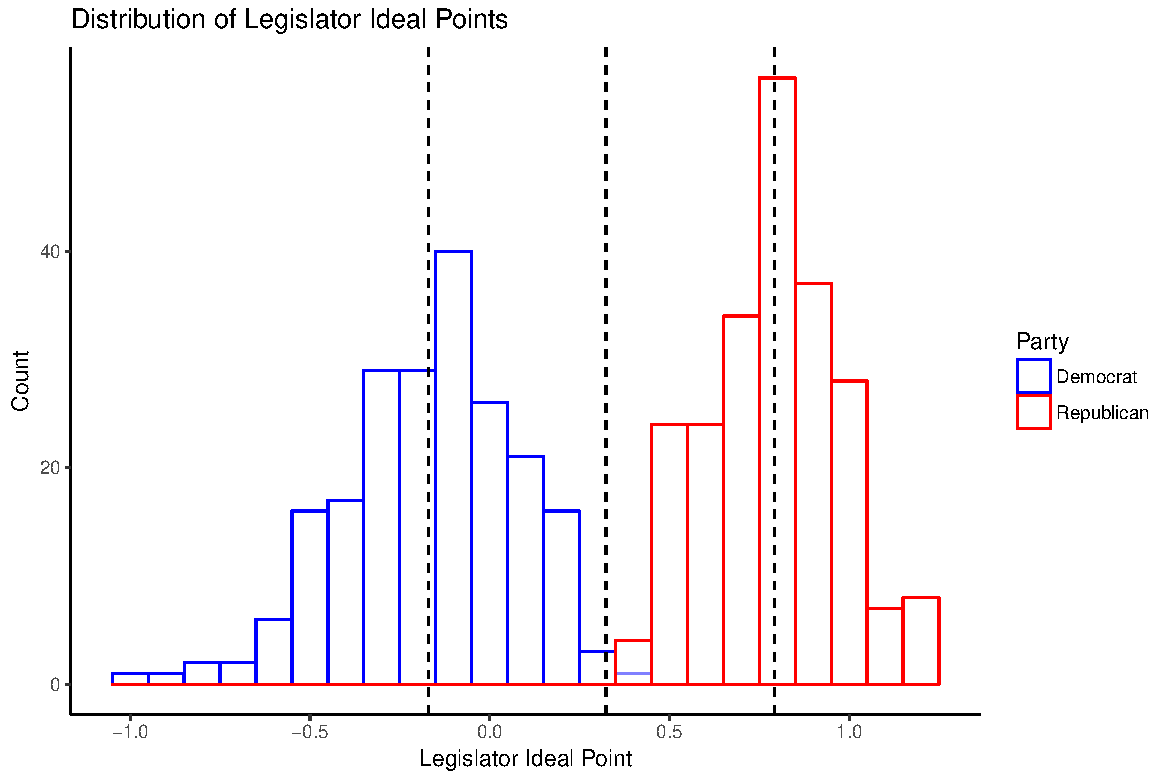
\includegraphics[width=.33\textwidth]{/Users/dsimp/GitHub/Clinton(2006)Rep/drafts/histogram/histogram-1} &
    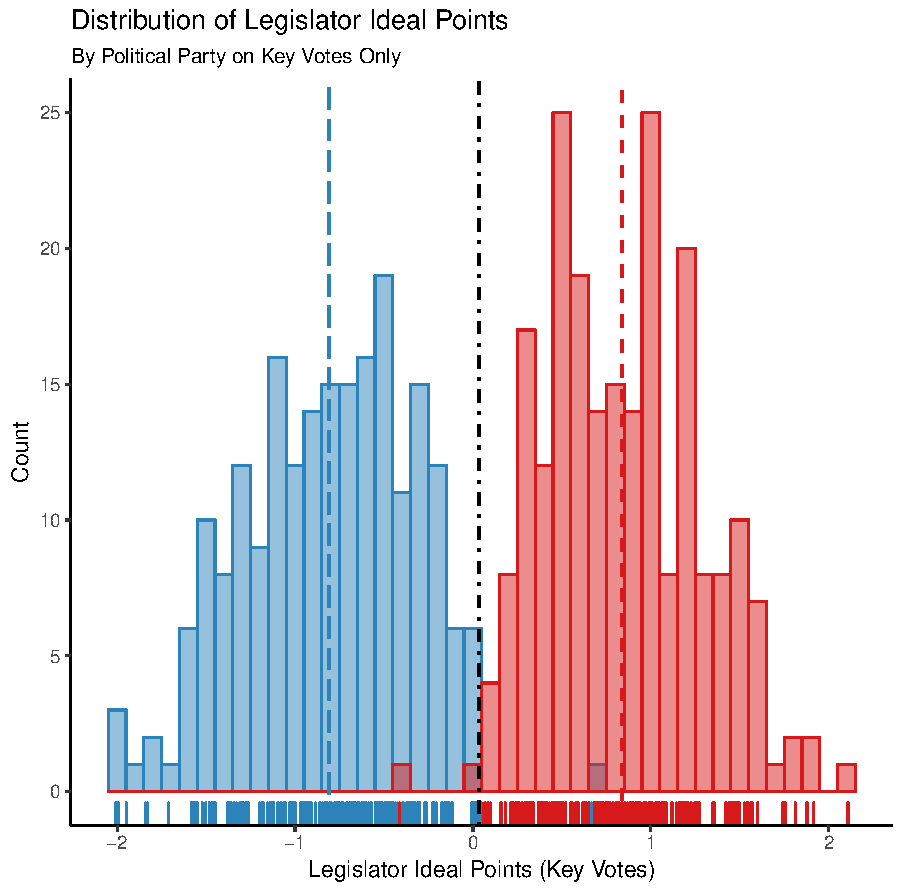
\includegraphics[width=.33\textwidth]{/Users/dsimp/GitHub/Clinton(2006)Rep/drafts/histogram/histogram-2} &
    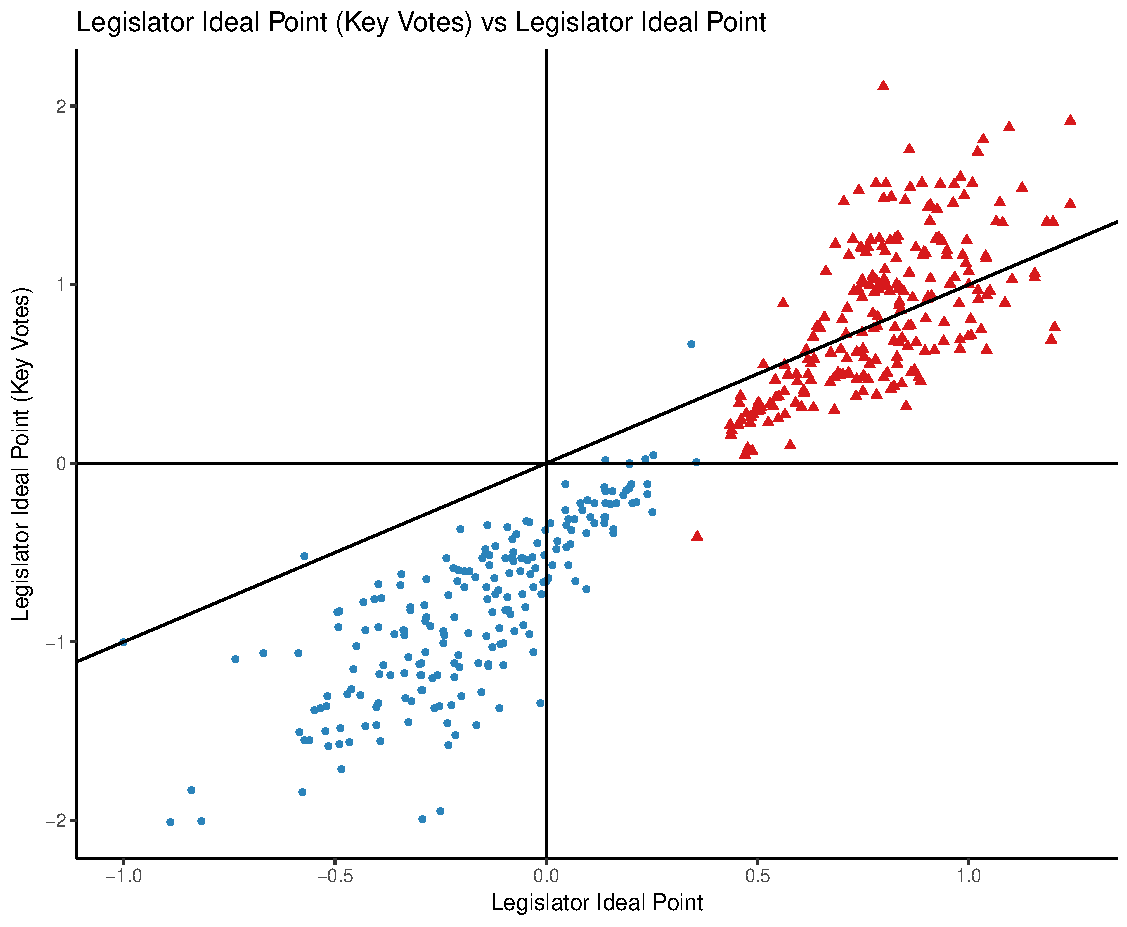
\includegraphics[width=.33\textwidth]{/Users/dsimp/GitHub/Clinton(2006)Rep/drafts/histogram/histo_change} \\
     & &  \\
    \small (D) District Mean Ideology &
    \small (E) Same-Party Mean Ideology &
    \small (F) Non-Same-Party Mean Ideology  \\
	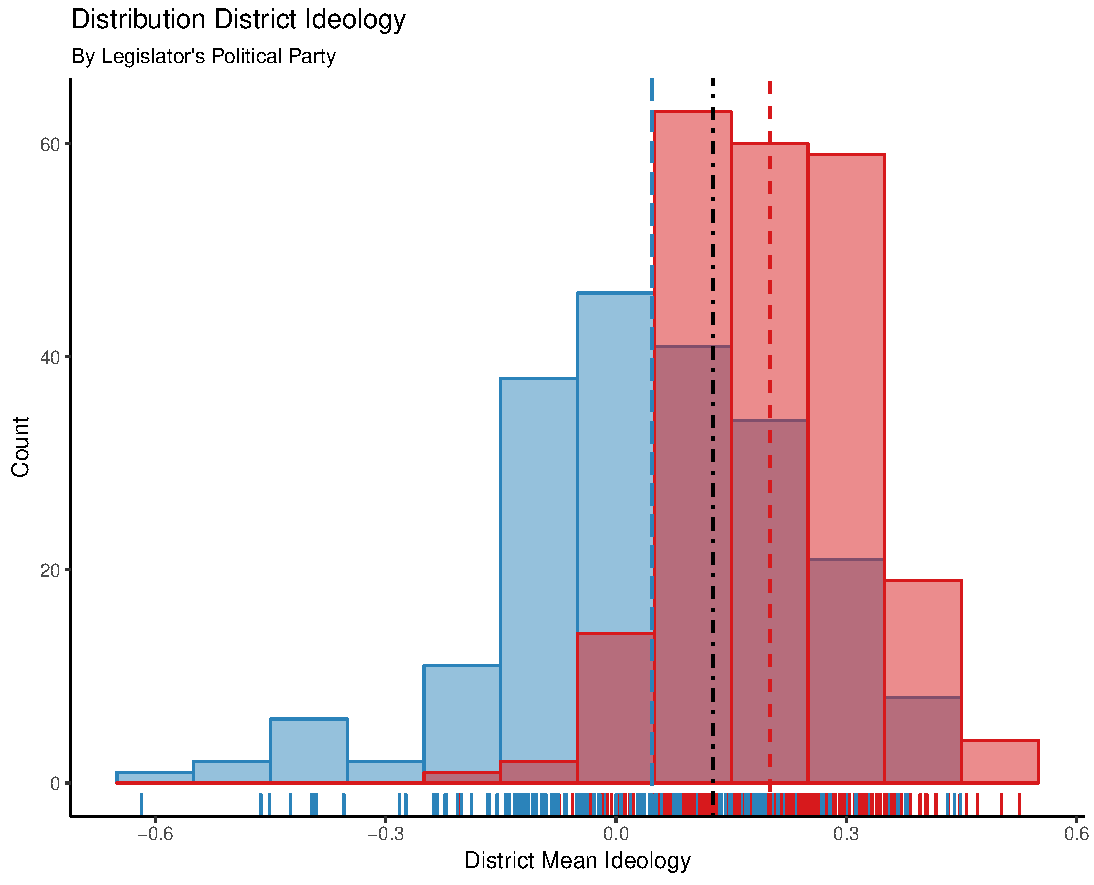
\includegraphics[width=.33\textwidth]{/Users/dsimp/GitHub/Clinton(2006)Rep/drafts/histogram/histogram-3} &
    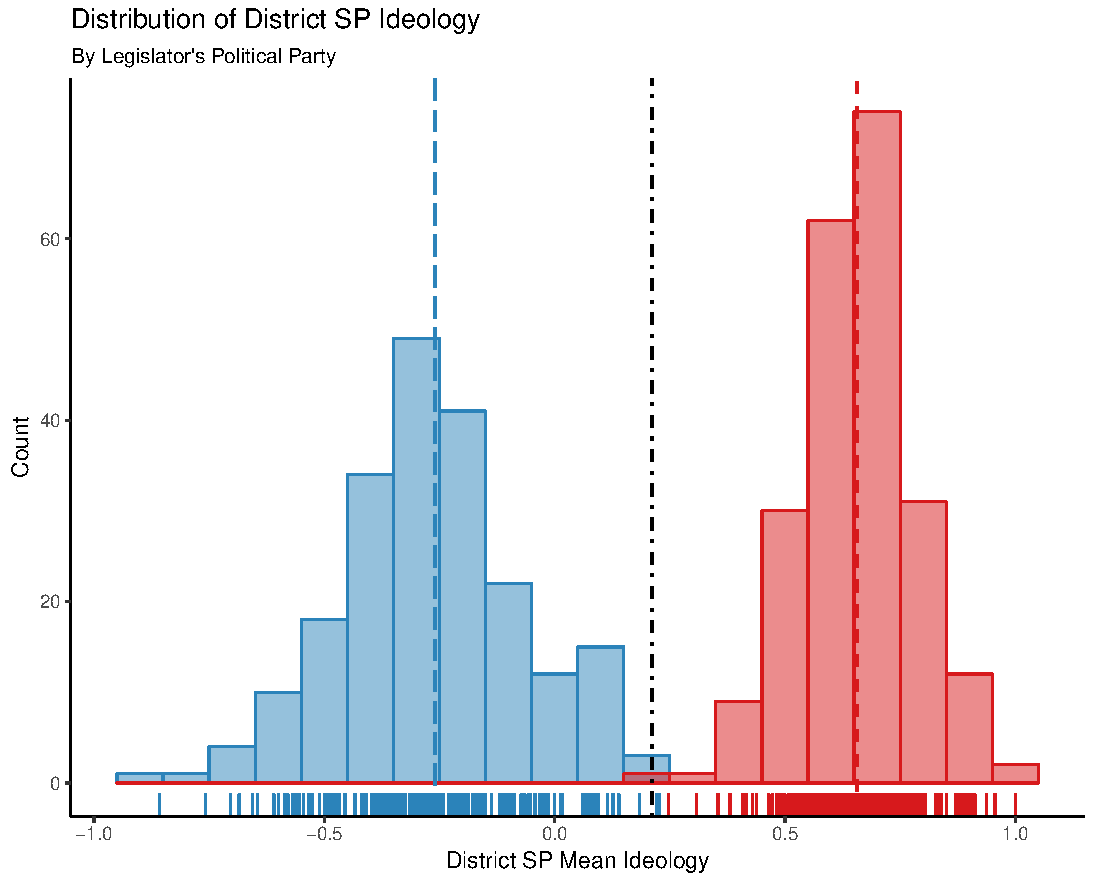
\includegraphics[width=.33\textwidth]{/Users/dsimp/GitHub/Clinton(2006)Rep/drafts/histogram/histogram-4} &
    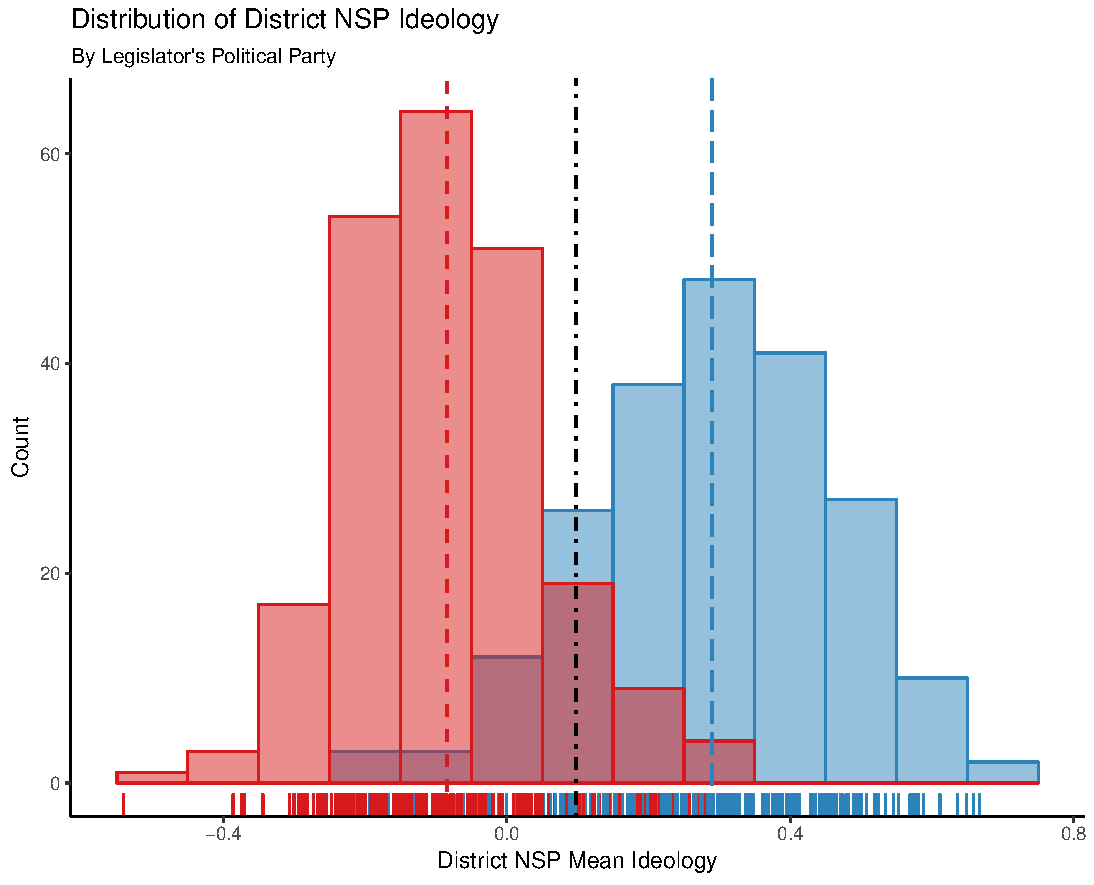
\includegraphics[width=.33\textwidth]{/Users/dsimp/GitHub/Clinton(2006)Rep/drafts/histogram/histogram-5} \\
      & &  \\
    \small (G) Opposite Party Mean Ideology&
    \small (H) Independent Mean Ideology&
    \small (I) Opposite Party vs Independent  \\
    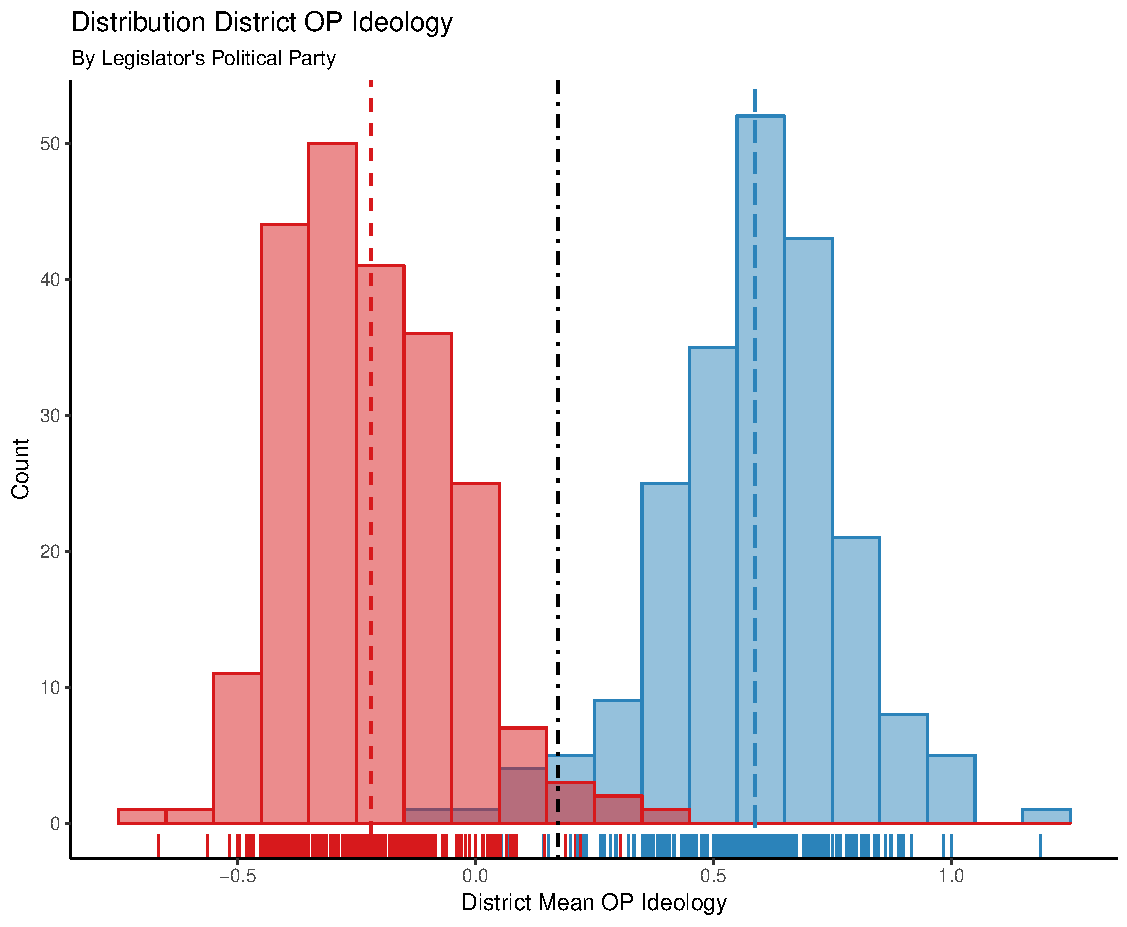
\includegraphics[width=.33\textwidth]{/Users/dsimp/GitHub/Clinton(2006)Rep/drafts/histogram/histogram-6} &
    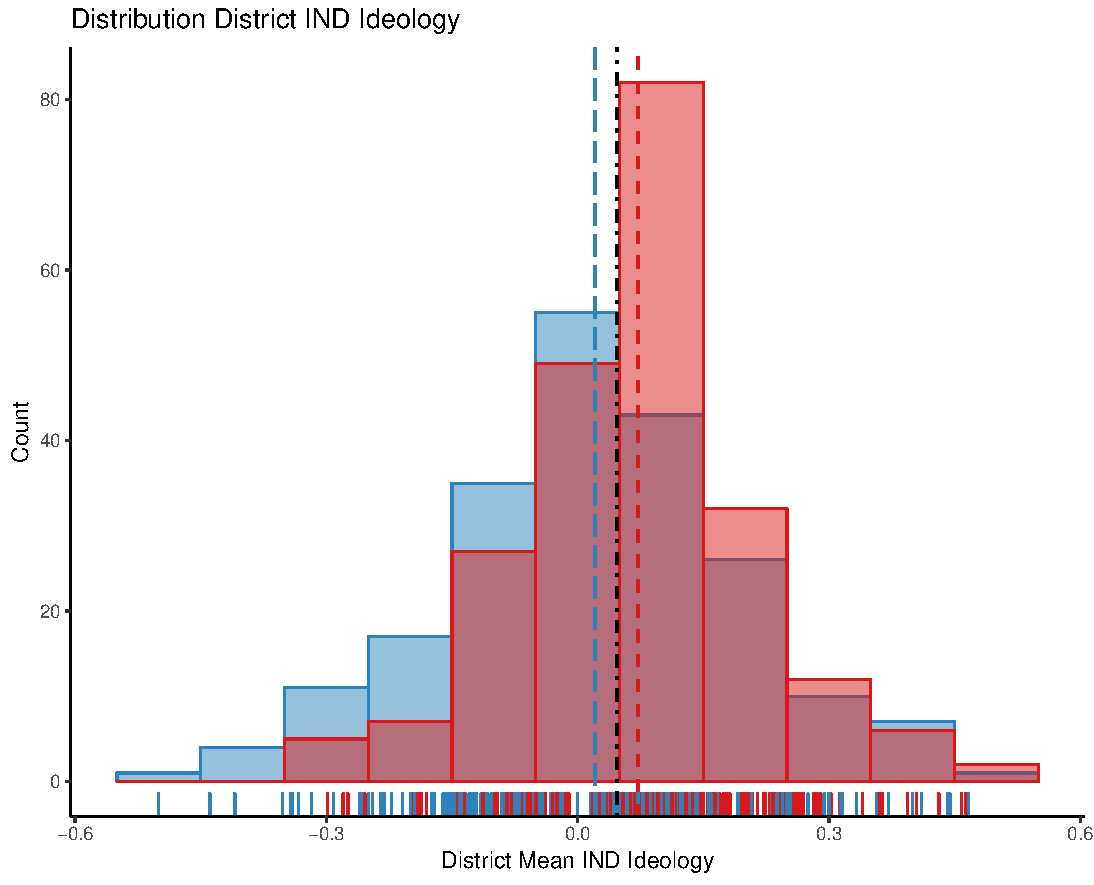
\includegraphics[width=.33\textwidth]{/Users/dsimp/GitHub/Clinton(2006)Rep/drafts/histogram/histogram-7} &
    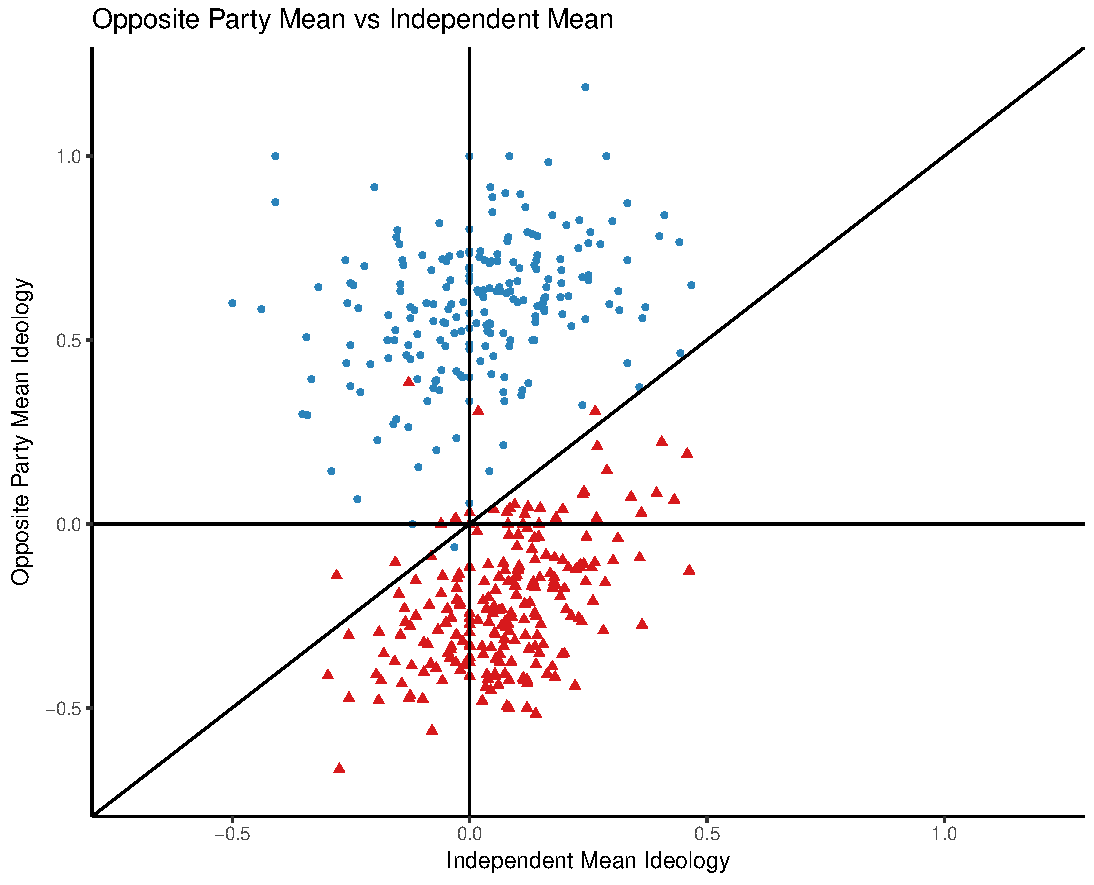
\includegraphics[width=.33\textwidth]{/Users/dsimp/GitHub/Clinton(2006)Rep/drafts/histogram/histo_diff} \\
       & &  \\
  \end{tabular}
    %}   
 \end{centering}\\
  \small \textbf{Note:} The histograms illustrate the distribution of legislator ideal points and sub-district constituency mean ideology grouped by legislator party. For histograms, the short dashed lines are the Republican means, the long dashed line are the Democratic means, and the dotted and dashed line is the chamber mean. Plot (C) shows the change in district district ideal point when key votes are used instead of all votes. Points above (below) the 45-degree line are more conservative (liberal) when key votes are used. Plot (I) compares district independent mean ideology to district opposite party mean ideology. Members with points above (below) the 45-degree line have opposite party constituents more conservative (liberal) than their independent constituents. 
\end{figure} 

The signaled vs revealed phenomenon is similar to but distinct from the delegate paradox described by \cite{Broockman2016} and \cite{Ahler2018}. As stated above, the delegate paradox indicates that a vote index can exaggerate the degree of extreme partisanship in a legislative chamber by making moderate legislators appear as extreme ideologues. The paradox is one of the many reasons why \textbf{Lax, Phillips and XXX} use for XYZ analysis. \textbf{Broockman and Ahler} state that the delegate paradox illustrates that an index is more reflective of ideological consistency rather than ideological extremity \textbf{(cite p. N)}. Since the signaled vs revealed phenomenon relies on a index of votes it is important to interpret the index scores as capturing consistency rather than extremity. Similar to Ahler and Broockman (2018)'s findings, the signaled vs. revealed phenomenon suggests ideology indices are sensitive to the inclusion of vote type (\textbf{fix to be sensitive to what is included.} The phenomenon is unique and novel because it suggests that ideological consistency as measured by key votes differs from ideological consistency as measured by all votes in a way that is predictable using existing theory of Congressional law making and legislative bargaining. The sensitivity is demonstrated by value differences in index values when key votes are used rather than all votes. Since all votes in an index are given equal weight, legislators may intentionally or unintentionally use inconsequential votes to shape the ideology of their signaled ideal point. However, key votes may reveal a more accurate reflection of ideological consistency.

There are elements of the above findings that fit within what might be expected during an era of split government. Cameron (XXXX)'s analysis of veto bargaining suggests that the president should be able to extract <xx>. As such, there is reason to believe that key votes are \textbf{blah.} As suggested by \textbf{Name (XXXX)}, there is reason to expect the set of all votes includes many votes intended for ideological signaling. Therefore, it is possible Democrats use these votes to signal bipartisan credibility and Republicans to use these votes to signal partisan reliability. In the context of the Cartel Model of Congress, it is expected that the majority of votes that receive a floor vote are \textbf{blah.}


\textbf{(1)} The Cartel Model of Congress indicates that we should expect floor votes in Congress to reflect BLAH. \textbf{(2)} As pointed out by XYZ, we should expect the distribution of votes across all votes to differ from that of Key Votes. If a high share of the total votes are either unimportant or are intended for ideological signaling, then we might expect the few votes of high importance to have a less conservative distribution. In fact, under split government with a Republican held House and a Democratic President we should also expect the average \textbf{Blank to shift toward the left.} Though we might expect both of these to be true, I cannot separate out this effect \textbf{at this time. At the time of writing, I do not have access to the full data set.} \textbf{CLean uP} Furthermore, it would be interesting to see how voting behavior changes in different Congresses and when the Democratic Party has agenda control.

Panels (D) through (H) plot histograms for district mean ideology scores and sub-district group mean ideology scores. Unlike legislator ideal points, the district ideology scores are measured using a 5 point ideology scale and are therefore a better reflection of ideological extremity (\textbf{see Data section cite Clinton and A and B.}). Each panel is separated into two groups: districts with Republican legislators and districts with Democratic legislators. Panel (D) shows that districts with Democratic legislators have a mean score that is more liberal than the average district and more liberal than the average district with a Republican legislator. However, Democratic legislators represent districts with mean ideology scores ranging from very liberal to very conservative. Panel (E) shows that same-party constituents are more polarized than the districts as a whole. 

Panels (F) through (H) show that classifying opposite party constituents and independents as a single non-same-party group masks two distinct underlying distributions and makes non-same-party constituents appear less polarized than same-party constituents. Rather, opposite-party constituents (panel G) are nearly as polarized as same-party constituents. \footnote{The left red (right blue) histogram plots the distribution of opposite-party constituents in districts with a Republican (Democratic) legislator.}The two distributions of independent voters reveals that independent voters are much less polarized than their partisan counterparts.\footnote{A Welch's t-test reveals the difference of means between independents in Republican and Democratic districts is statistically significant. However, it is notable that the distributions of independent mean ideologies are both much closer to a mean of zero.} The mean and standard deviations of the ideology scores are given in Appendix Table A2. Table A2 also contains summary statistics for the group shares of each sub-district constituency as a percent of total district constituents. Appendix Figure A1 plots the distribution of sub-district constituent group shares. The average share of same-party constituents in Republican held districts is 0.39, in Democratic held districts it is 0.45. The standard deviation of same-party shares in Democratic districts is nearly twice that of Republican held districts. As such, it is reasonable to expect that independents play a unique role in districts where legislators must compete for both same-party constituents and independents to reach a majority.

Lastly, Panel (I) plots district independent independent ideology against opposite-party ideology. In general, independents in Republican (Democratic) held districts are more conservative (liberal) than the respective opposite-party constituents. The split is evidence using the 45-degree line. Points above (below) the line indicate that independents are more liberal (conservative) than opposite-party constituents.

\textbf{Figure 2} depicts twelve simple regression plots that explore the relationship between the primary variables of interest. In each panel, districts represented by a Republican (Democrat) are plotted with a red triangle (blue circle). A bivariate trend line is added for district level analysis, and a trend lines are included for district analysis by party control. With the exception of panel (I), the slope of the overall trend lines differs substantially from the slopes of the party specific trend lines. Together the plots illustrate the necessity for analysis that includes differences by party - especially since some overall trend lines suggest a negative relationships among the considered variable pairings. In contrast, each pairing demonstrates a positive relationship when analyzed by party.

Panels (A) through (E) plot legislator ideal points (all votes) against district mean ideology and sub-district constituent group ideology. Panel (A) is particularly interesting because it illustrates that Republican and Democratic legislators with similar district ideologies vote differently. Clinton (2006) states that such a plot indicates that geographic constituency preferences alone cannot explain voting behavior (p. 401). A point that I agree with. Though, it is important to interpret the differences in terms of consistency rather than extremity. Additionally, panel (A) illustrates Clinton's observation that Democratic held districts are less homogeneous than Republican held districts. Panel (B) shows that legislator ideal points are consistently more conservative as district ideology becomes more conservative. 

Panels (C) through (E) illustrate show the relationships between independent and opposite party.

It is also important to note that missing from each of these plots is the share of each party group. It should be expected that legislators respond to both party ideology and party size. Indeed Appendix Figure 2A depicts the relationship between party ideology and party size. The panels clearly illustrate that representatives respond to group size.

Across all panels, it is evident that as constituent ideology becomes more conservative so does legislator ideal points.

Panels (F) through (I) illustrate that increases in district ideological conservativism is associated with increases in sub-district constituent group conservativism. However, there are still differences by party identification. For example, panel (F) shows that both Republican and Democrat same party constituent ideology has a positive linear relationship with district ideology, but as a whole Republican same-party constituents are more conservative than Democratic same-party constituents. Similarly, panel (H) shows a positive trend between opposite party ideology and district ideology. Though, opposite party constituents are \textbf{polarized}. In contrast, there seems to be no party effect for Independent voters. Average independent ideology is more conservative in more conservative districts; however, there does not seem to be an identifiable difference between independent ideology among districts with similar ideologies but different partisan representatives. \textbf{This finding is novel for two reasons. First, Table A2 indicates that on average the share of same-party constituencies is less 50\% for districts with legislators of either party. (Though Democratic districts have a larger same-party mean and standard deviation). Second, A2 indicates that independent ideology is less partisan. As such, it should be expected that legislators of each party do have to compete for independent votes.} Therefore, this provides additional evidence that we should not classify independent voters together with opposite party voters.

Panels (J) through (L) plot sub-constituent ideologies against same party ideologies. \textbf{Explanation}. Plot (L) indicates that Independents in Republican districts are more liberal than self-identified Republicans. Similarly, most Independents in Democratic districts are more conservative than self-identified Democrats. Though the relationship is not uniform. For districts with similar same-party ideologies, there are both liberal and conservative mean independents. \textbf{fix sentence.}

\textbf{Finish up!}


\newpage
\begin{figure}[!htbp]
\caption{Legislator Ideal Points and District Ideology Means}
\begin{centering}
%\centering
%\fbox{
  \begin{tabular}{@{}ccc@{}}
	% & & \\  	
  	\small (A) Ideal Point &
    \small (B) Ideal Point &
    \small (C) Ideal Point  \\
    \small vs District Ideology & 
    \small vs Same-Party Ideology &
    \small vs Non-Same-Party Ideology \\
    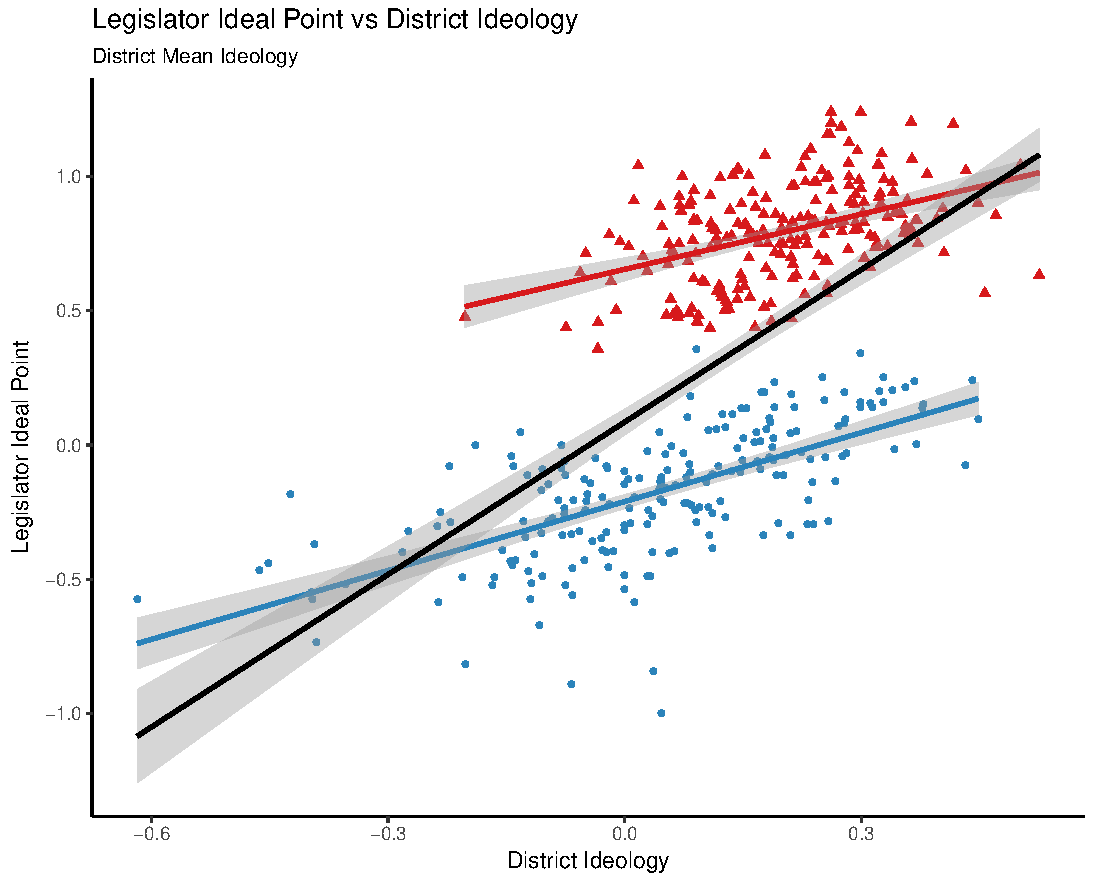
\includegraphics[width=.30\textwidth]{/Users/dsimp/GitHub/Clinton(2006)Rep/drafts/plots/plot1-1.pdf} &
    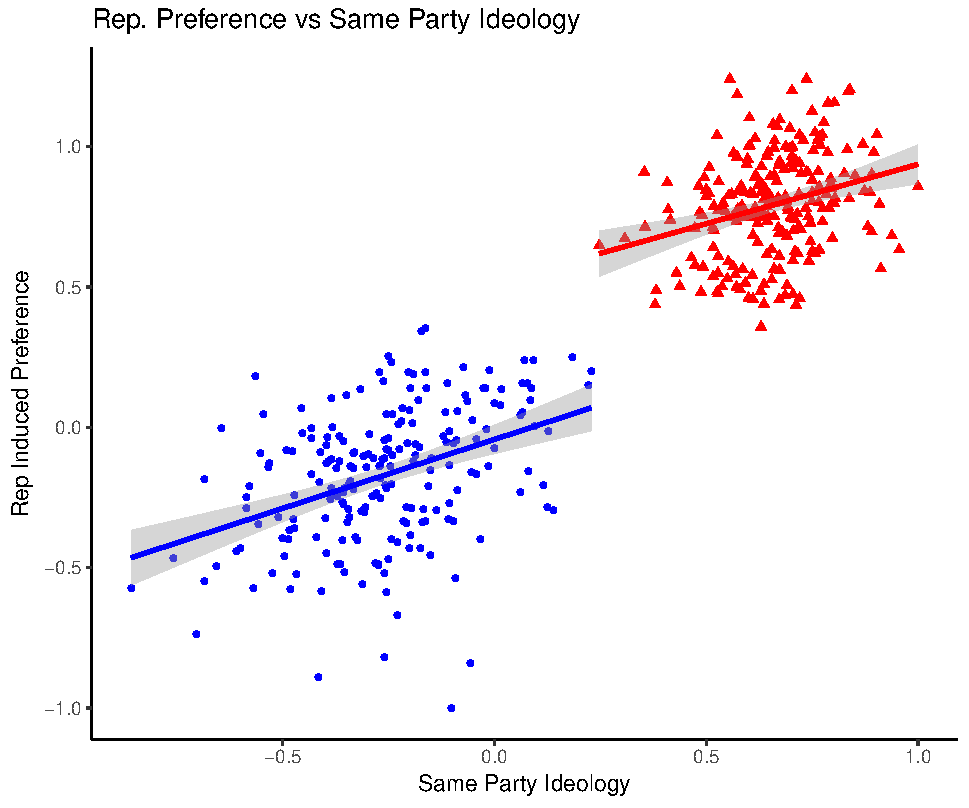
\includegraphics[width=.30\textwidth]{/Users/dsimp/GitHub/Clinton(2006)Rep/drafts/plots/plot1-2.pdf} &
    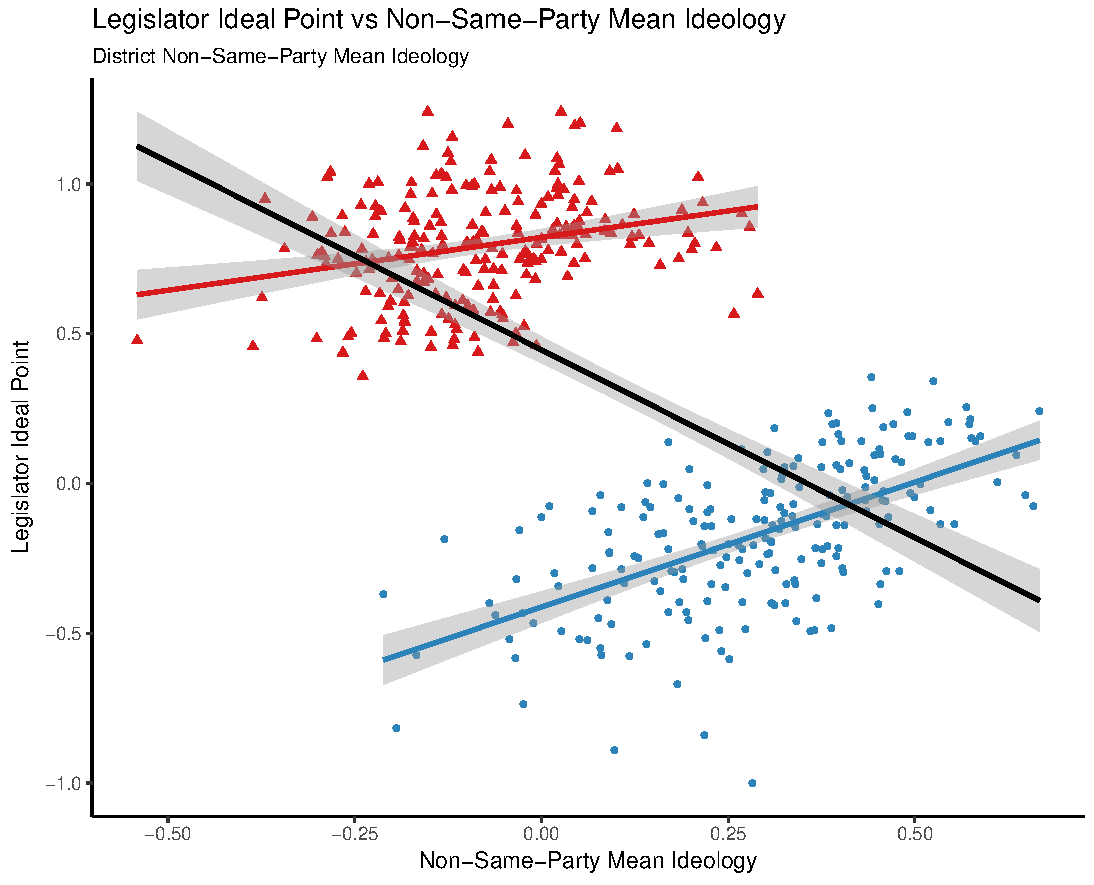
\includegraphics[width=.30\textwidth]{/Users/dsimp/GitHub/Clinton(2006)Rep/drafts/plots/plot1-3.pdf} \\
    % & & \\
    \small (D) Ideal Point & 
    \small (E) Ideal Point & 
    \small (F) Same-Party Ideology  \\
    \small vs Opposite Party Ideology  & 
    \small vs Independent Ideology  & 
    \small vs District Ideology \\
    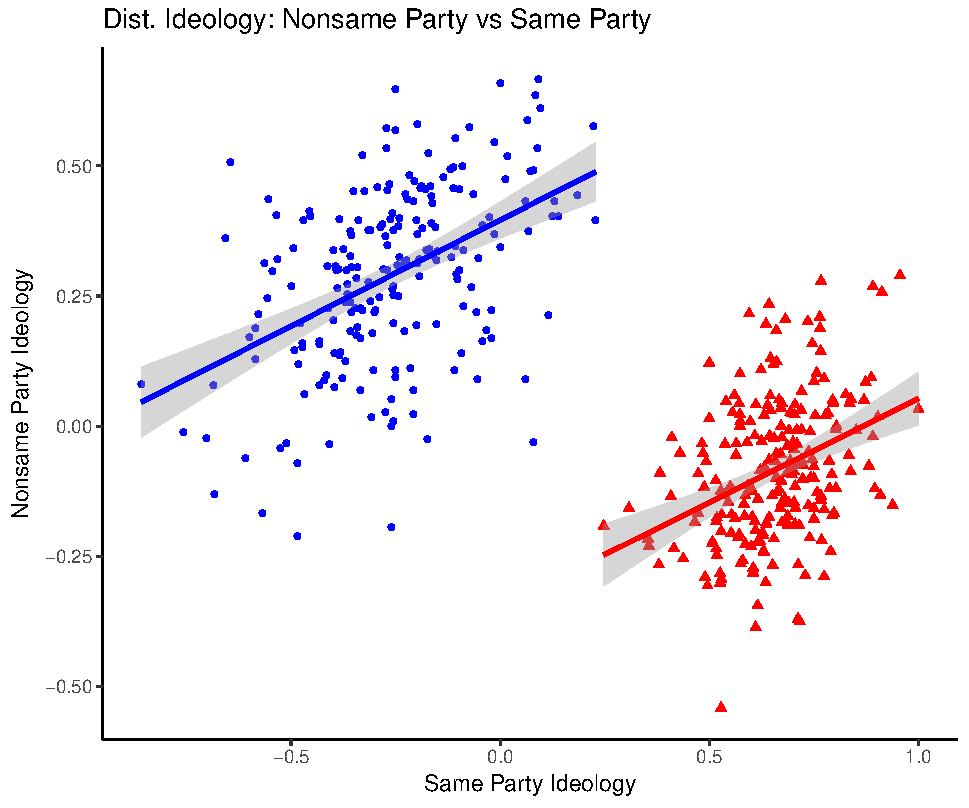
\includegraphics[width=.30\textwidth]{/Users/dsimp/GitHub/Clinton(2006)Rep/drafts/plots/plot1-4.pdf} &
    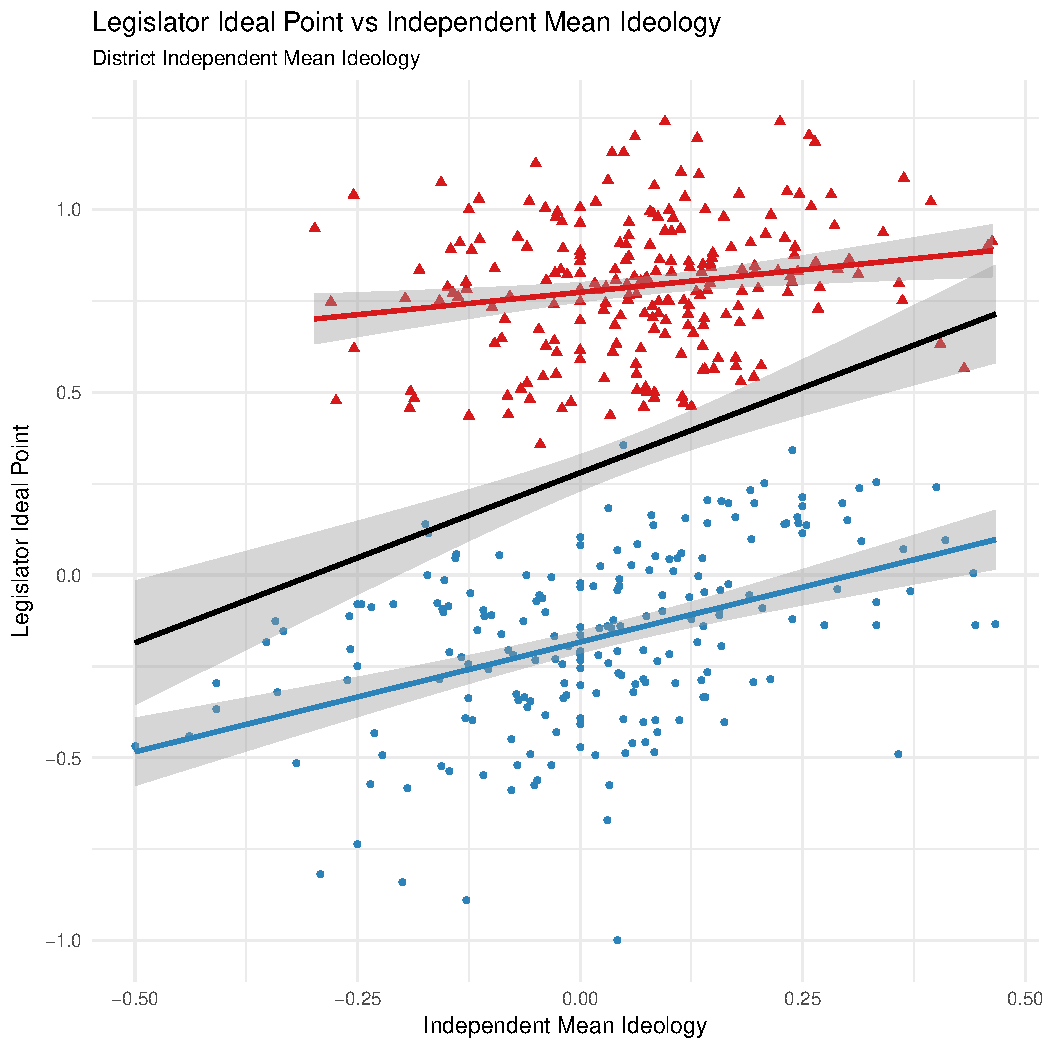
\includegraphics[width=.30\textwidth]{/Users/dsimp/GitHub/Clinton(2006)Rep/drafts/plots/plot1-5.pdf} &
    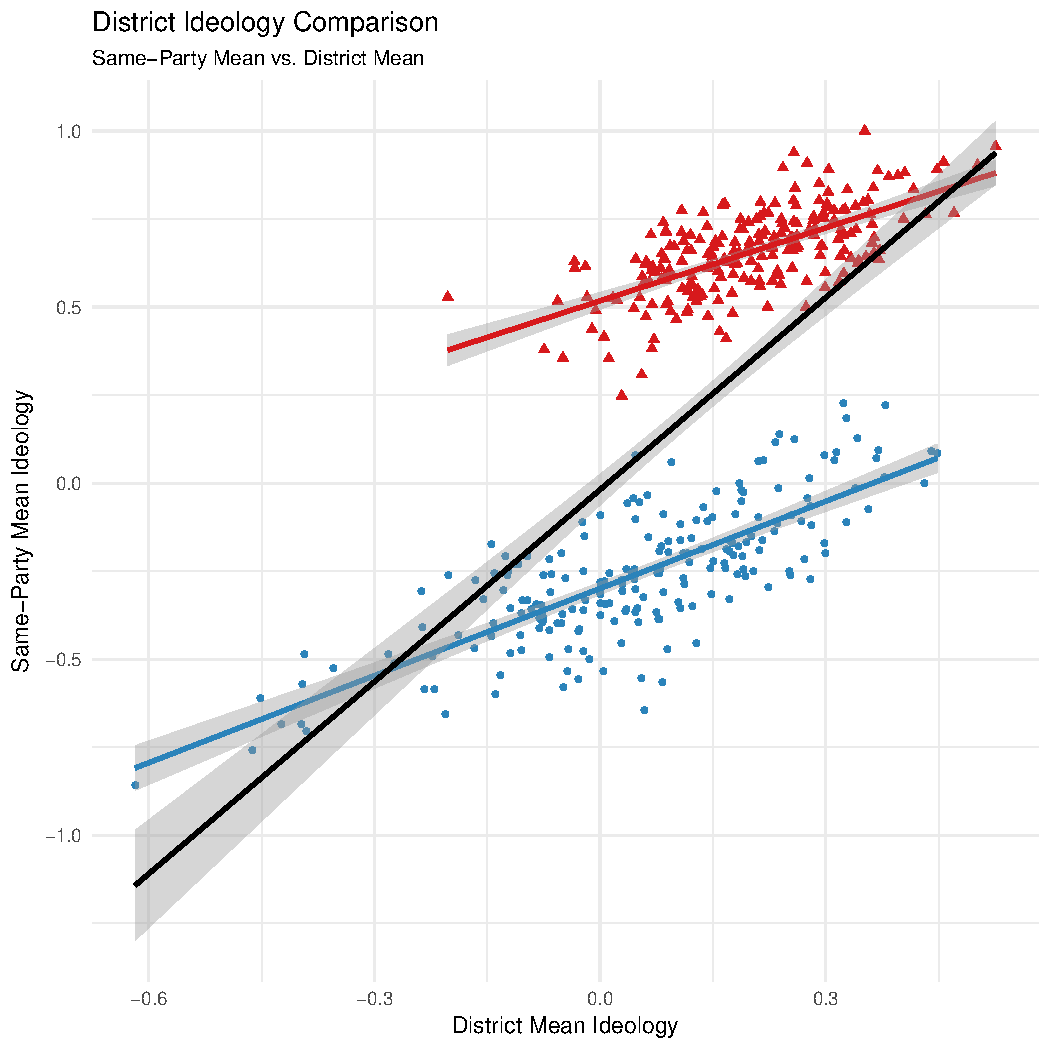
\includegraphics[width=.30\textwidth]{/Users/dsimp/GitHub/Clinton(2006)Rep/drafts/plots/plot1-6.pdf} \\
    % &  &\\
    \small (G) Non-Same-Party Ideology & 
    \small (H) Opposite Party Ideology & 
    \small (I) Independent Ideology  \\
    \small vs District Ideology  & 
    \small vs District Ideology  & 
    \small vs District Ideology \\
    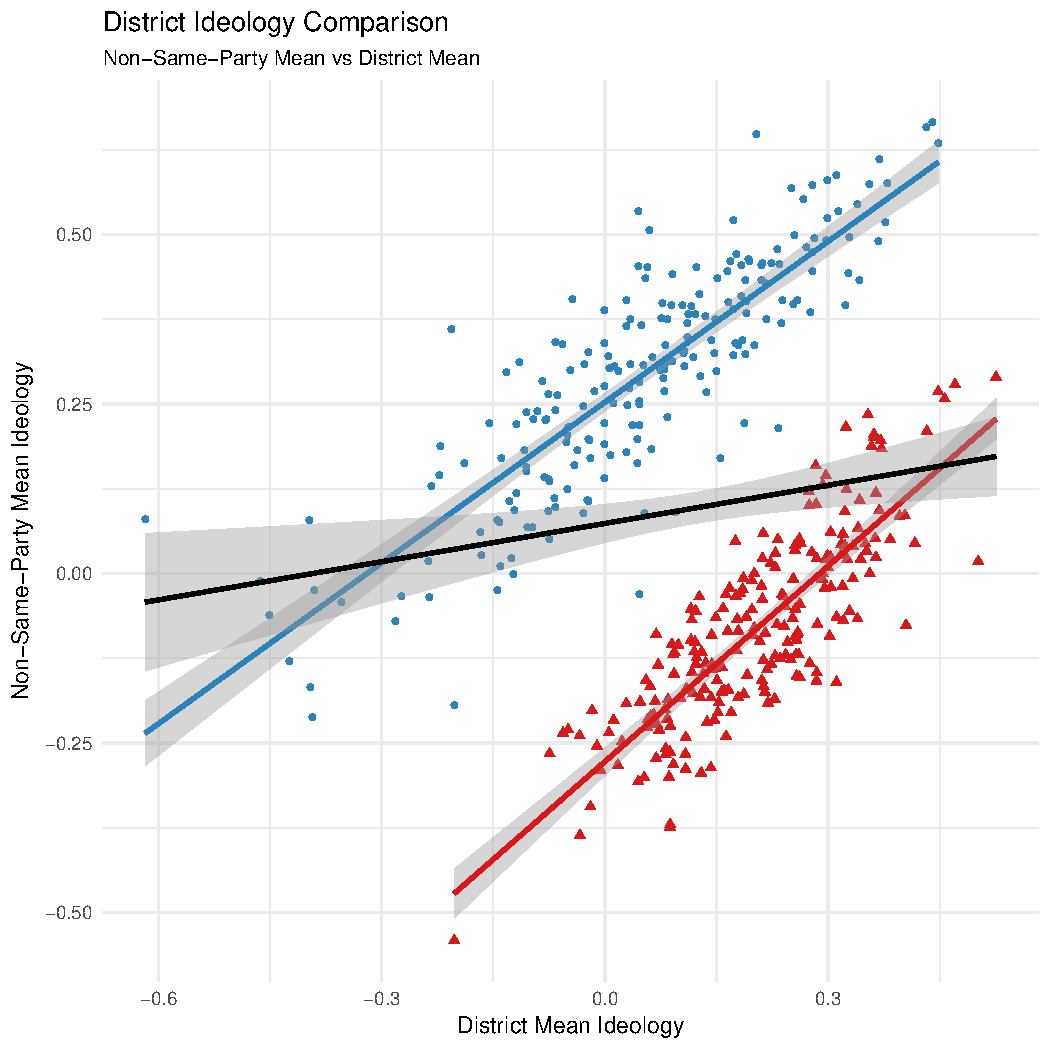
\includegraphics[width=.30\textwidth]{/Users/dsimp/GitHub/Clinton(2006)Rep/drafts/plots/plot1-7.pdf} &
    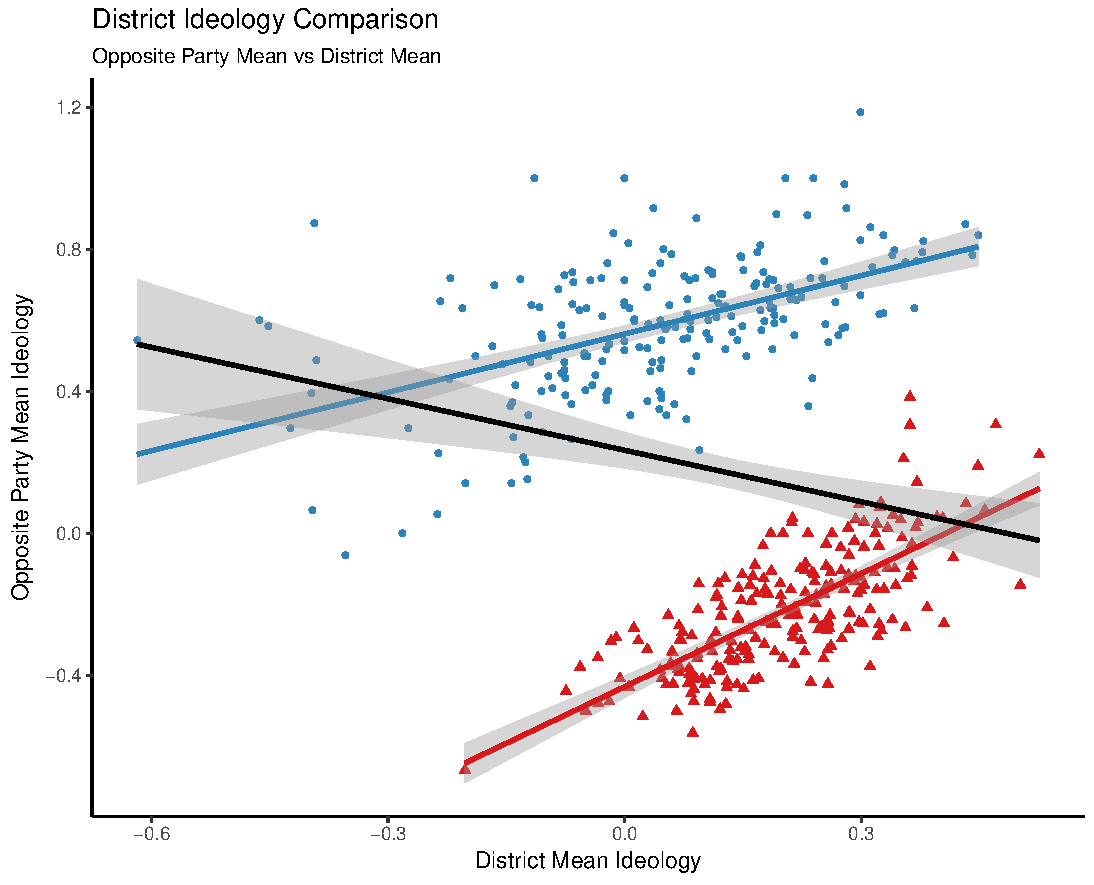
\includegraphics[width=.30\textwidth]{/Users/dsimp/GitHub/Clinton(2006)Rep/drafts/plots/plot1-8.pdf} &
    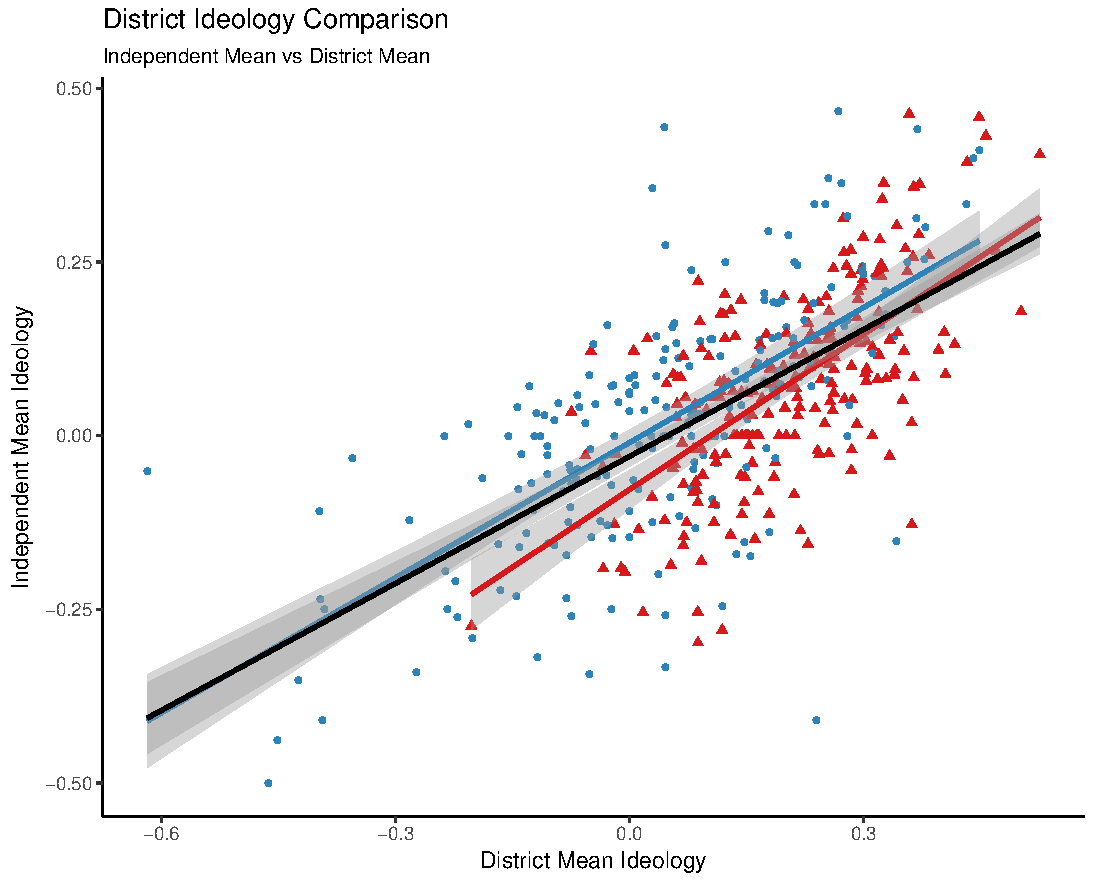
\includegraphics[width=.30\textwidth]{/Users/dsimp/GitHub/Clinton(2006)Rep/drafts/plots/plot1-9.pdf} \\
    % &  &\\
    \small (J) Non-Same-Party Ideology & 
    \small (K) Opposite Party Ideology & 
    \small (L) Independent Ideology  \\
    \small vs Same-Party Ideology  & 
    \small vs Same-Party Ideology  & 
    \small vs Same-Party Ideology \\
    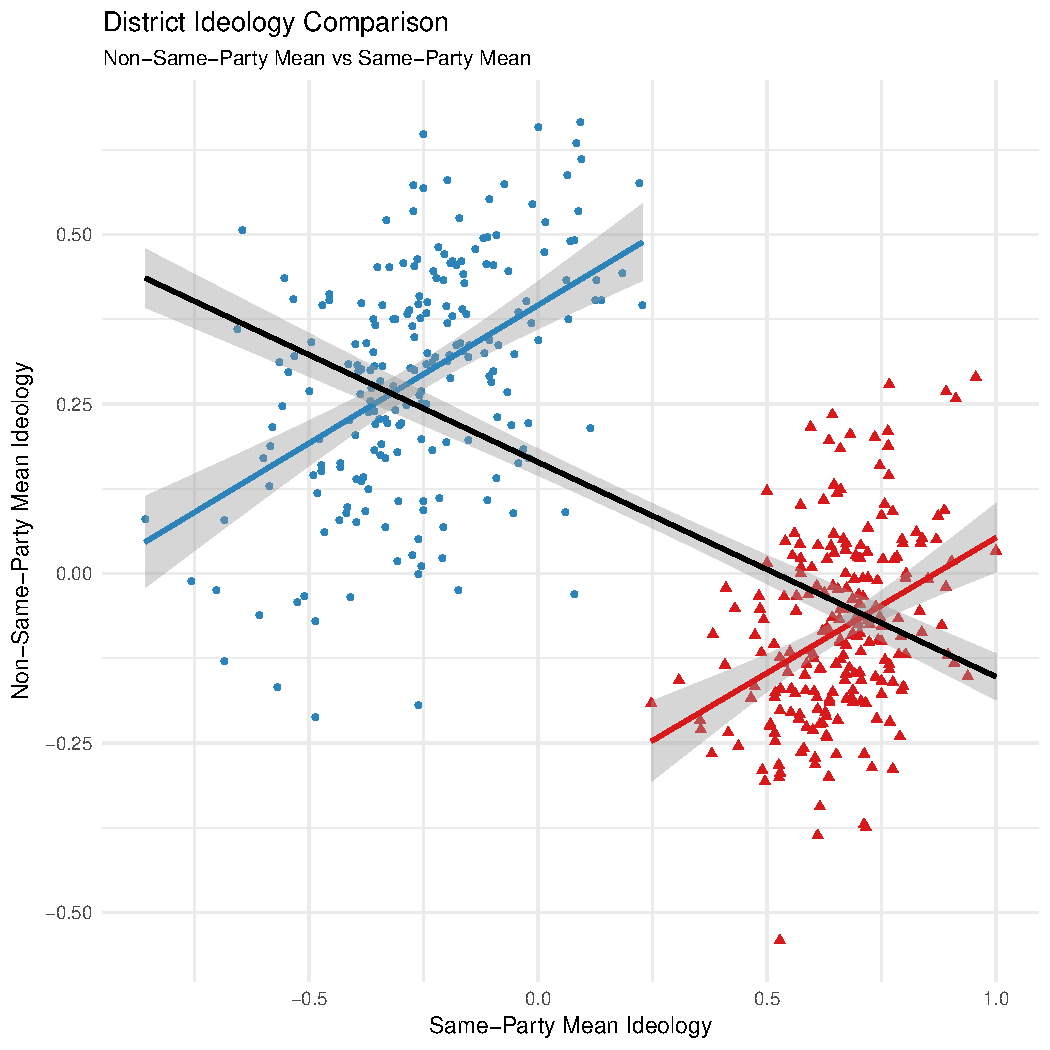
\includegraphics[width=.30\textwidth]{/Users/dsimp/GitHub/Clinton(2006)Rep/drafts/plots/plot1-10.pdf} &
    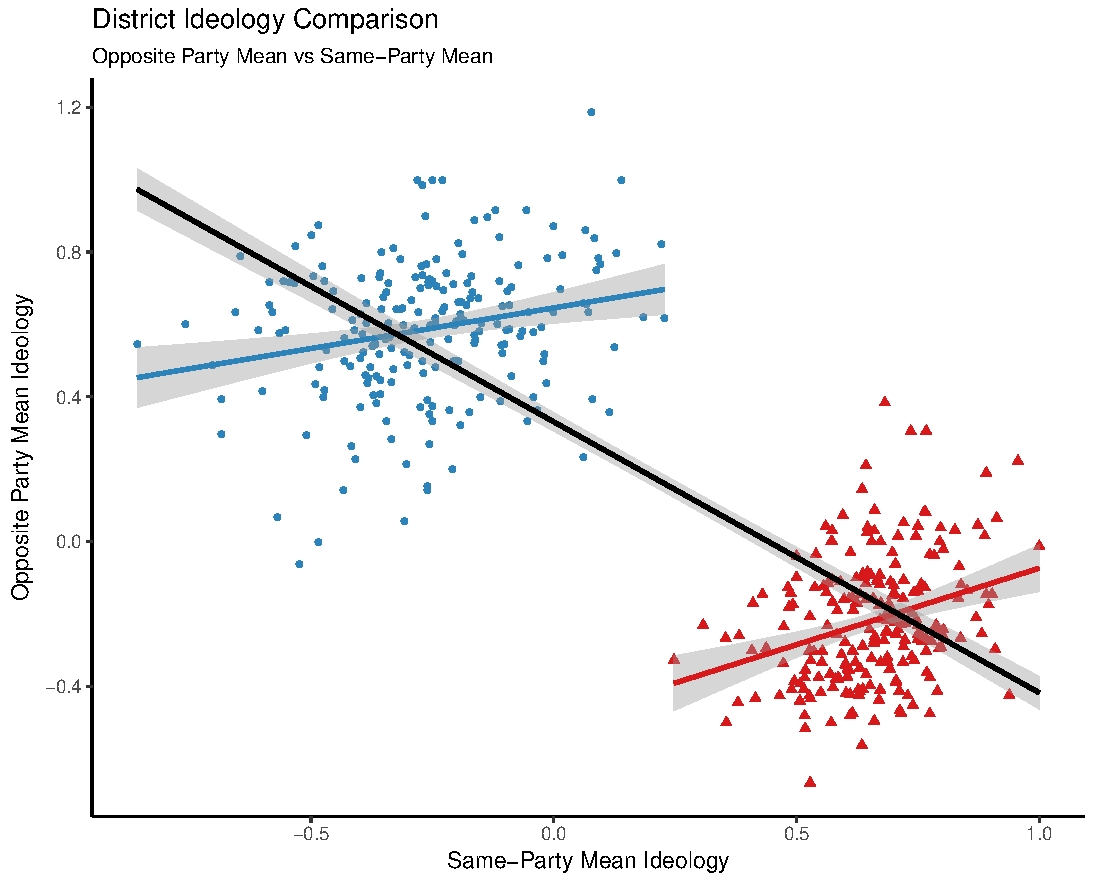
\includegraphics[width=.30\textwidth]{/Users/dsimp/GitHub/Clinton(2006)Rep/drafts/plots/plot1-11.pdf} &
    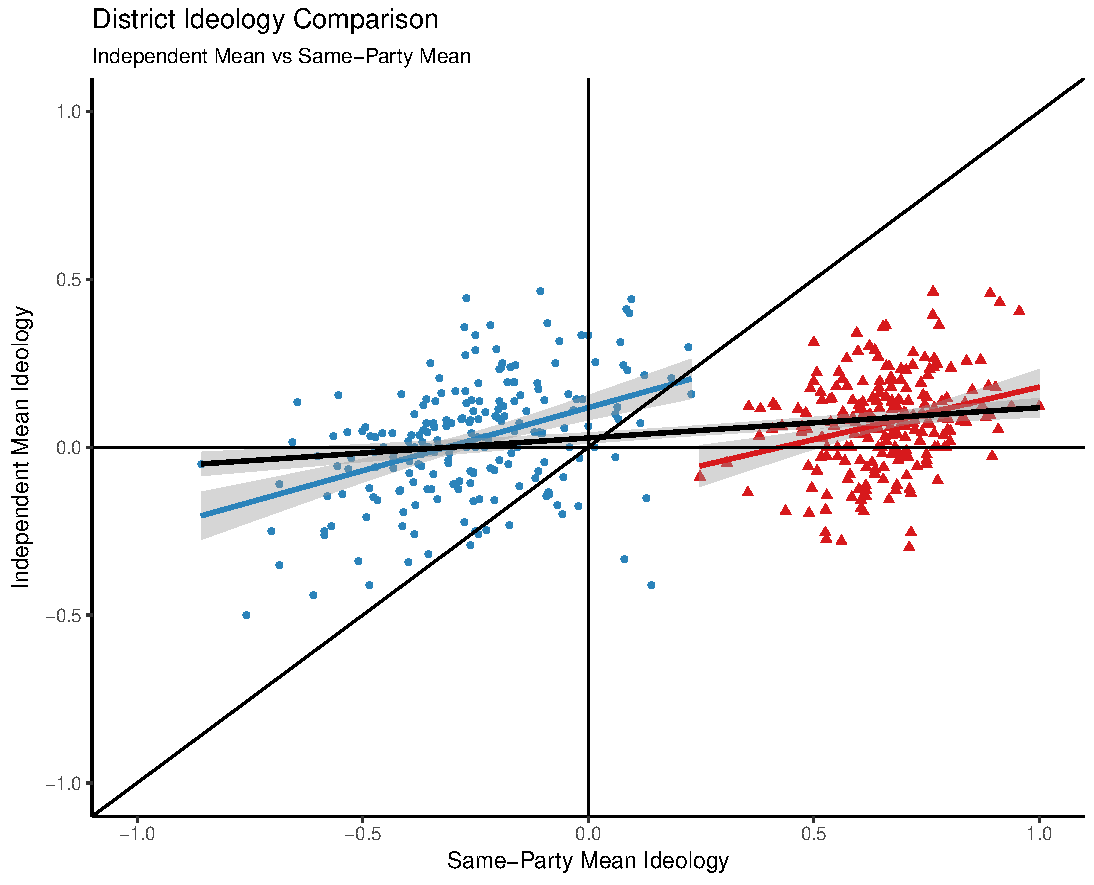
\includegraphics[width=.30\textwidth]{/Users/dsimp/GitHub/Clinton(2006)Rep/drafts/plots/plot1-12.pdf} \\
  \end{tabular}
    %}   
 \end{centering}
 \small \textbf{Note:} Districts represented by Republicans (Democrats) are plotted with triangles (circles). A bivariate trend line is plotted for overall comparison and party trend lines are plotted for comparison within districts.
\end{figure} 
\newpage

\section{Initial Findings} 

\subsection{Interaction Terms}
The main empirical issue in \citep{Clinton2006} is that each model with interaction terms omits the constitutive terms necessary for determining the relationship between sub-district ideology and legislator ideal point. \cite{Brambor2006} demonstrate that there is almost never a valid reason to omit constitutive variables when a model includes interaction terms. Observe the below equation (1) which appears in Clinton's Table 1. The model regresses legislator ideal points ($y_i$) on weighted sub-district level average ideology scores. The terms $w_{SP_i}$ and $w_{NSP_i}$ respectively weight same-party average ideology ($\bar{z}_{SP_i}$) and non-same-party average ideology ($\bar{z}_{NSP_i}$) by the share of group members sampled in each district. As such, the weights in equation (1) are defined $w_{SP_i} = \frac{n_i^{SP}}{n_i}$ and $w_{NSP_i} =  \frac{n_i^{SP}}{n_i}$. The term $I_{GOP}$ is a party indicator variable. 

\begin{equation}
y_i  = \beta_0 + \beta_1 w_{SP_i} \bar{z}_{SP_i} + \beta_2 w_{NSP_i} \bar{z}_{NSP_i} + \gamma I_{GOP} + \varepsilon_i
\end{equation}
This specification is incorrect and yields biased coefficient values and underestimated coefficient standard errors. The correct specification of model (1) should include $w_{SP_i}$, $w_{NSP_i}$, $\bar{z}_{SP_i}$, $\bar{z}_{SP_i}$ each as individual independent variables in addition to their interaction. As such, the correctly specified model is given in the below equation (2).
\begin{equation}
\begin{array}{ccc}
y_i & = & \alpha_0 + \alpha_1 w_{SP_i} \bar{z}_{SP_i} + \alpha_2 w_{NSP_i} \bar{z}_{NSP_i} + \alpha_3 \bar{z}_{SP_i}~~~~~~~~~\\ 
& & ~~+ \alpha_4 \bar{z}_{NSP_i} + \alpha_5 w_{SP_i} + \alpha_6 w_{NSP_i} + \lambda I_{GOP} + \epsilon_i
\end{array}
\end{equation}
Equation (1) implies that one can estimate the unconditional marginal effect of weighted group ideology (i.e. $\beta_1$ for the single term $\big( \frac{n_i^{SP}}{n_i} \bar{z}_{SP_i}\big)$ and that neither the weights nor sub-district group ideologies have an independent effect on legislator ideal point. That is, equation (1) implicitly assumes that $\alpha_3$, $\alpha_4$, $\alpha_5$, and $\alpha_6$ from equation (2) are all zero. Empirically, this is incorrect. Intuitively, one should expect group size $w_{j\in \{SP,NSP\}_i}$ and group ideology $\bar{z}_{j\in \{SP,NSP\}_i}$ to individually influence legislator behavior. One should also expect the impact of group share (group ideology) to change as group ideology (share) changes.

Empirically, the marginal effect of group share (group ideology) is given by the derivative of legislator ideal point with respect to share (ideology). For example in equation (2), the relationship between legislator ideal point and same-party ideology is: 
$$\frac{\partial y_i}{\partial \bar{z}_{SP_i}}= \alpha_1 w_{SP_i} + \alpha_3$$
The coefficient $\alpha_3$ captures the portion of the slope $\frac{\partial y}{\partial \bar{z}_{SP_i}}$ (the relationship between ideal point and same-party ideology) that is constant across all districts regardless of the district share of same-party constituents. The terms $\alpha_1 w_{SP_i}$ captures how the slope $\frac{\partial y}{\partial \bar{z}_{SP_i}}$ changes as the district share of same-party constituents increases. Therefore equation (2) is underspecified and the estimates of $\beta_1$ and $\beta_2$ will be biased. %For example, the coefficient $\beta_1$ on weighted same-party ideology in equation (1) is capturing $\alpha_1$, $\alpha_3$ and $\alpha_5$ from equation (4). % Uncomment to reinsert

Additionally, it is important to note that the use of interaction terms implies that a second calculation is necessary to determine the standard errors for the marginal effects of group share or group ideology. One cannot simply rely on usually reported coefficient values and standard errors to determine statistical significance of a variable that is included in an interaction term. Rather, it is necessary to directly calculate the variance term. For example, consider the marginal effect of same-party ideology. The variance is given as:  $var(\frac{\partial y}{\partial \bar{z}_{SP_i}})$. That is $var(\frac{\partial y}{\partial \bar{z}_{SP_i}}) = var(\alpha_1 w_{SP_i} + \alpha_4)$. Therefore, the standard error term for $\frac{\partial y}{\partial \bar{z}_{SP_i}}$ is given by:
$$\hat{\sigma}_{\partial y_i / \partial \bar{z}_{SP_i}} = \sqrt{w_{SP}^2var(\hat{\alpha}_1)+var(\hat{\alpha}_3)+2w_{SP}cov(\hat{\alpha}_1\hat{\alpha}_3)}$$

The below Table 1 provides the regression results for models 1 and 2. Model 1 is a replication of Clinton (2006)'s Table 1 Model 2. The Model 1 results replicated here are identical to those found in Clinton (2006). Model 2 is the correctly specified model with each of the interaction terms. However, Percent Same-Party and Percent Non-Same Party are perfectly multicolinear by construction. Therefore, Percent Non-Same-Party is omitted. Under this specification, one cannot estimate the marginal effect Percent Non-Same Party; however, Model 3 omits the constant term and allows for estimation of the marginal effect of Percent Non-Same Party.

$$Insert ~ Explanation~Of~Results~Here$$

Insert chart showing the difference of the regression predictions for the two models using same-party ideology and non-same party ideology. Include in the new figure 2.

Figure 3 provides an illustration of the marginal effects of group share and group ideology for both same- and non-same-party.

$$Insert ~ Explanation~Of~Results~Here$$

\input{/Users/dsimp/GitHub/Clinton(2006)Rep/drafts/stargazer/table2.txt}


\begin{figure}[!htbp]
\caption{Representative Ideal Points and District Ideology (Two Groups)}
\begin{centering}
%\centering
%\fbox{
  \begin{tabular}{@{}cc@{}}
	 & \\  
	\small (A) Marginal Effect of Percent Same-Party&	
  	\small (B) Marginal Effect of Same-Party Ideology\\
    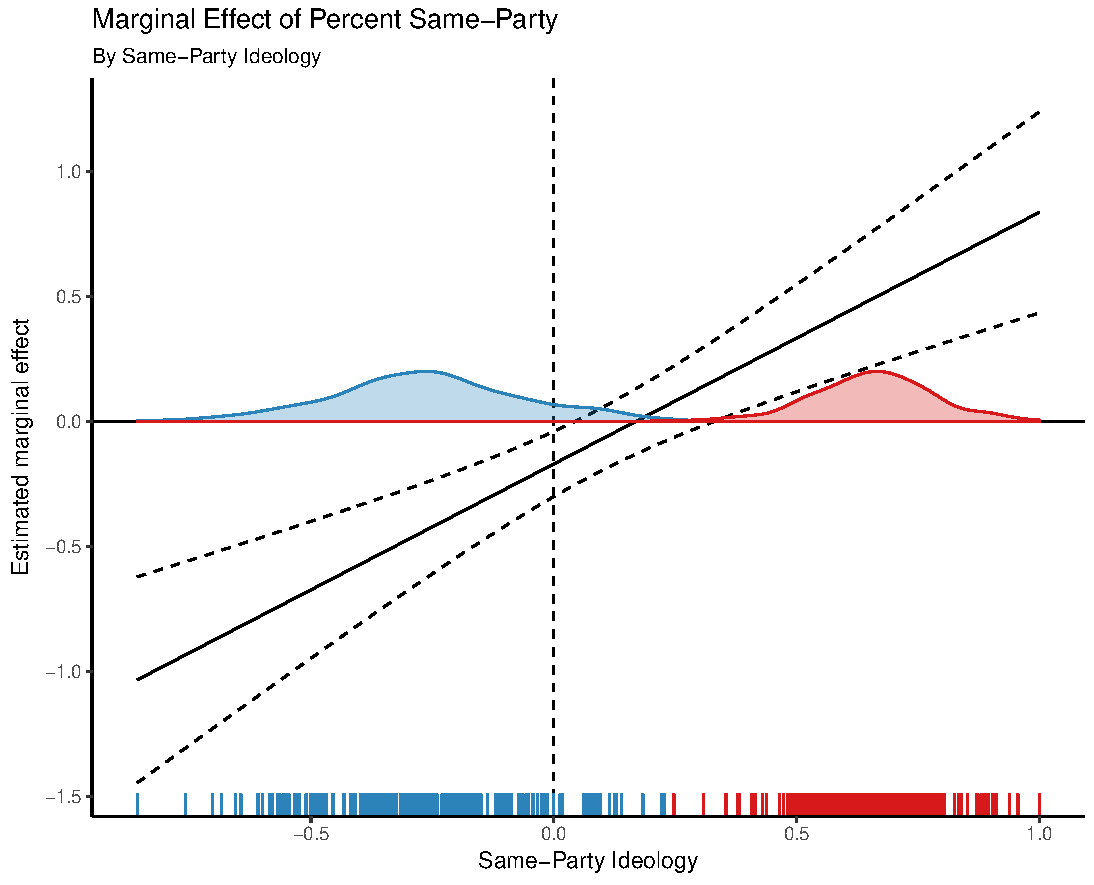
\includegraphics[width=.45\textwidth]{/Users/dsimp/GitHub/Clinton(2006)Rep/drafts/marginals/me-2.pdf} &
    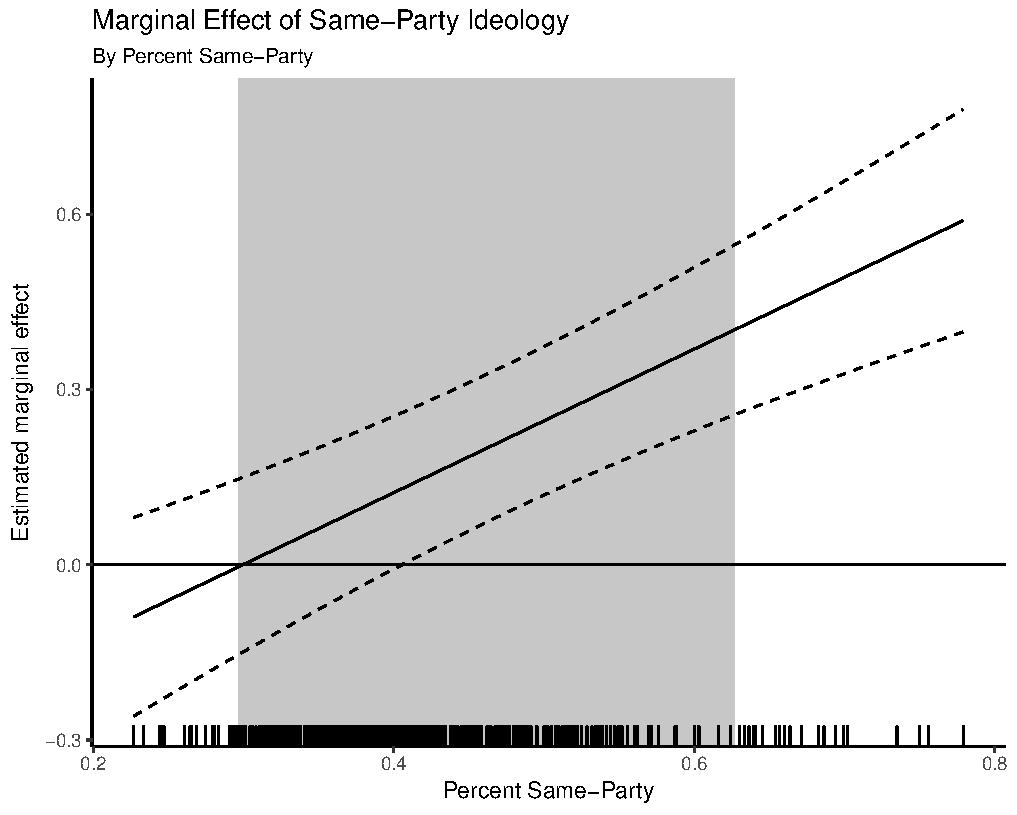
\includegraphics[width=.45\textwidth]{/Users/dsimp/GitHub/Clinton(2006)Rep/drafts/marginals/me-1.pdf} \\
     & \\
	\small (C) Marginal Effect of Percent Non-Same-Party& 
    \small (D) Marginal Effect of Non-Same-Party Ideology\\
    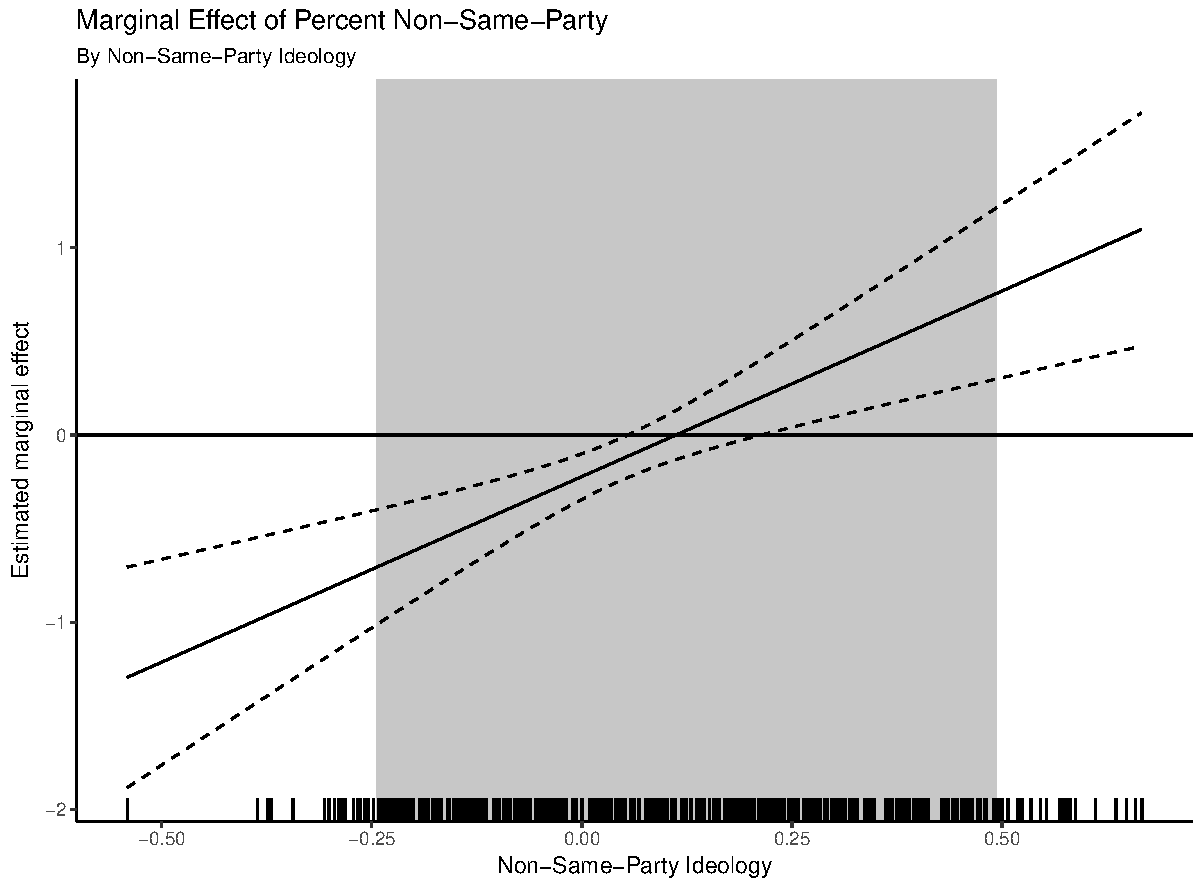
\includegraphics[width=.45\textwidth]{/Users/dsimp/GitHub/Clinton(2006)Rep/drafts/marginals/me-4.pdf} &
    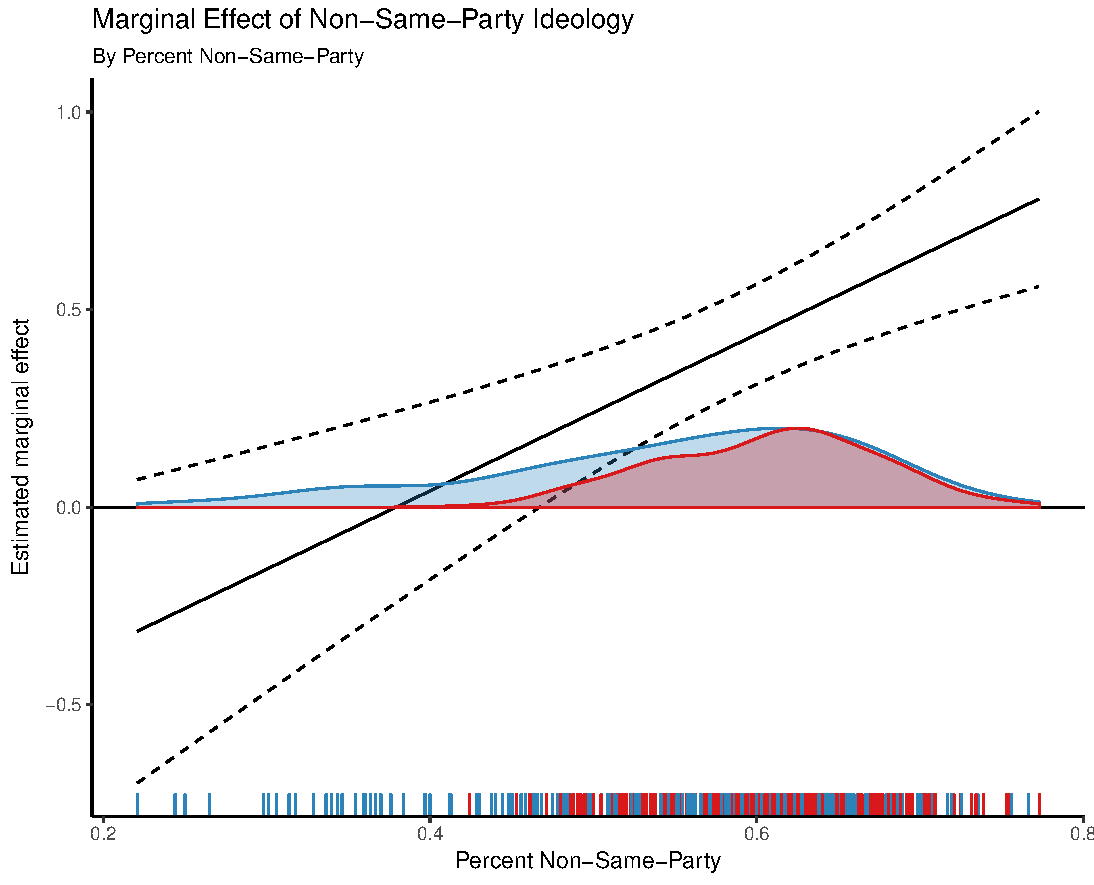
\includegraphics[width=.45\textwidth]{/Users/dsimp/GitHub/Clinton(2006)Rep/drafts/marginals/me-3.pdf} \\
     &  \\
  \end{tabular}
    %}   
 \end{centering}
  \textbf{Note:} Each panel plots the respective marginal effect of the constitutive terms of the interaction variables in Table 2 Model 3.
\end{figure}
 

\begin{figure}[!htbp]
\caption{Representative Ideal Points and District Ideology (Three Groups)}
\begin{centering}
%\centering
%\fbox{
  \begin{tabular}{@{}cc@{}}
	 & \\  	
	\small (A) Marginal Effect of Percent Same-Party&	
  	\small (B) Marginal Effect of Same-Party Ideology\\
    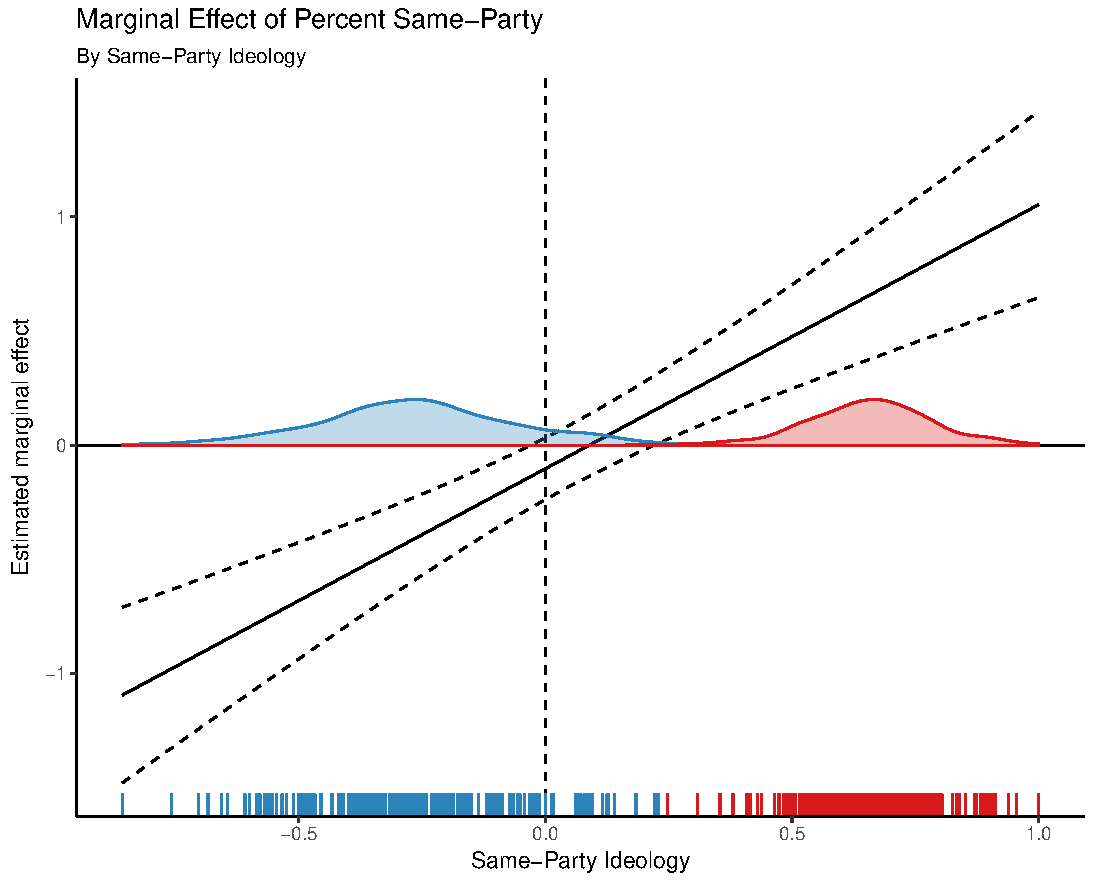
\includegraphics[width=.45\textwidth]{/Users/dsimp/GitHub/Clinton(2006)Rep/drafts/marginals/meb-1.pdf} &
    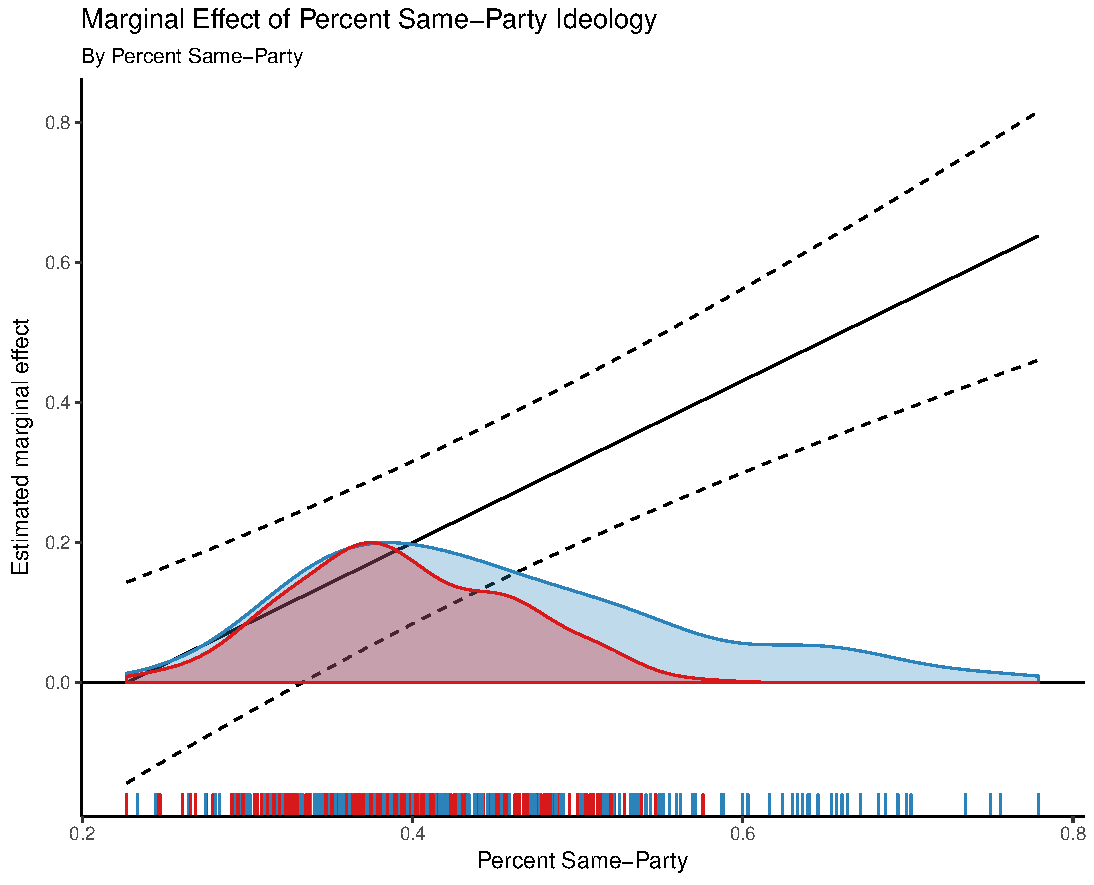
\includegraphics[width=.45\textwidth]{/Users/dsimp/GitHub/Clinton(2006)Rep/drafts/marginals/meb-2.pdf} \\
     & \\
	\small (C) Marginal Effect of Percent Independent& 
    \small (D) Marginal Effect of Independent Ideology\\
    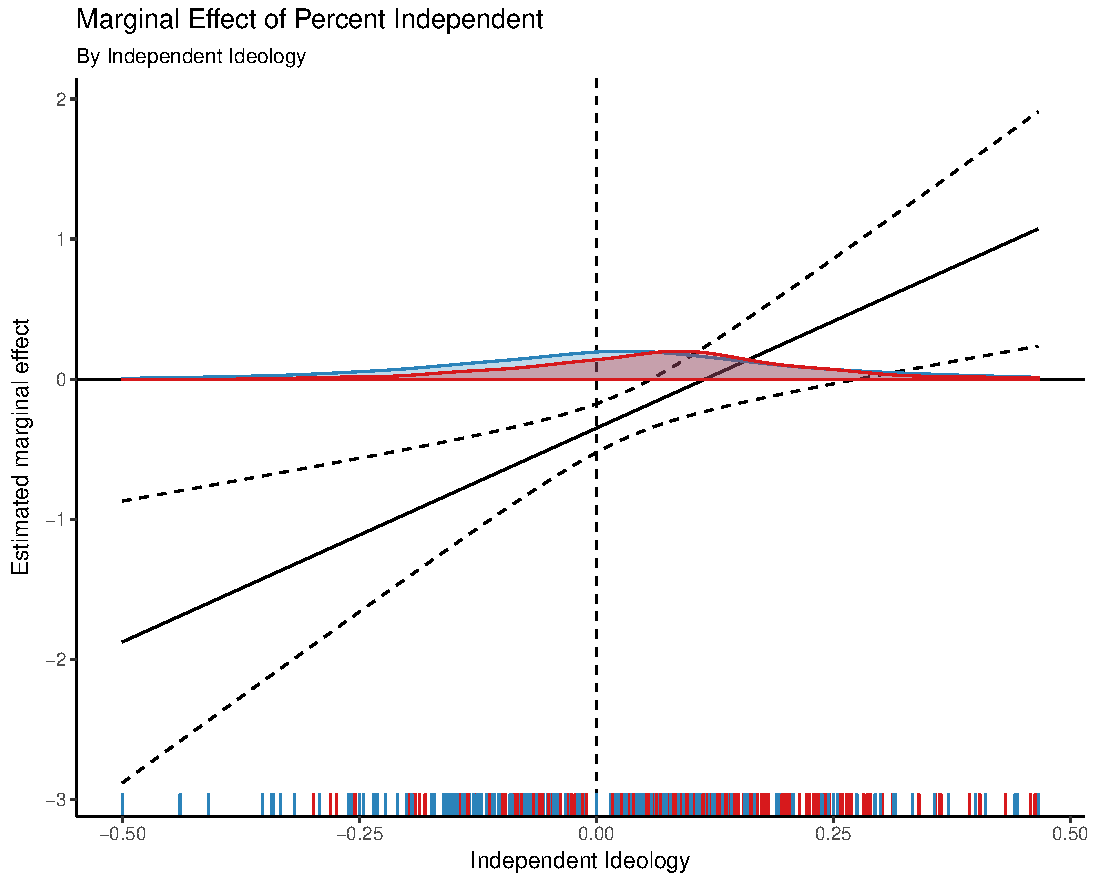
\includegraphics[width=.45\textwidth]{/Users/dsimp/GitHub/Clinton(2006)Rep/drafts/marginals/meb-3.pdf} &
    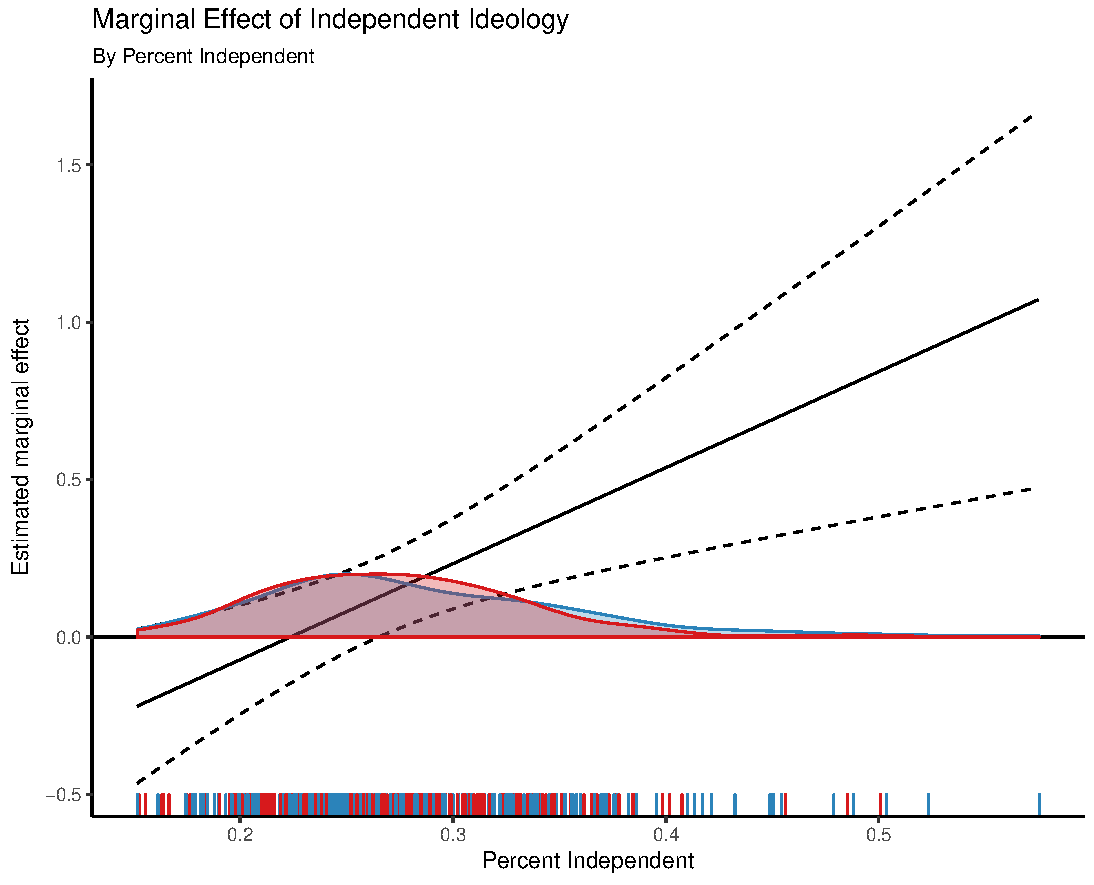
\includegraphics[width=.45\textwidth]{/Users/dsimp/GitHub/Clinton(2006)Rep/drafts/marginals/meb-4.pdf} \\
     &  \\
    \small (E) Marginal Effect of Percent Opposite-Party&  
    \small (F) Marginal Effect of Opposite-Party Ideology\\
    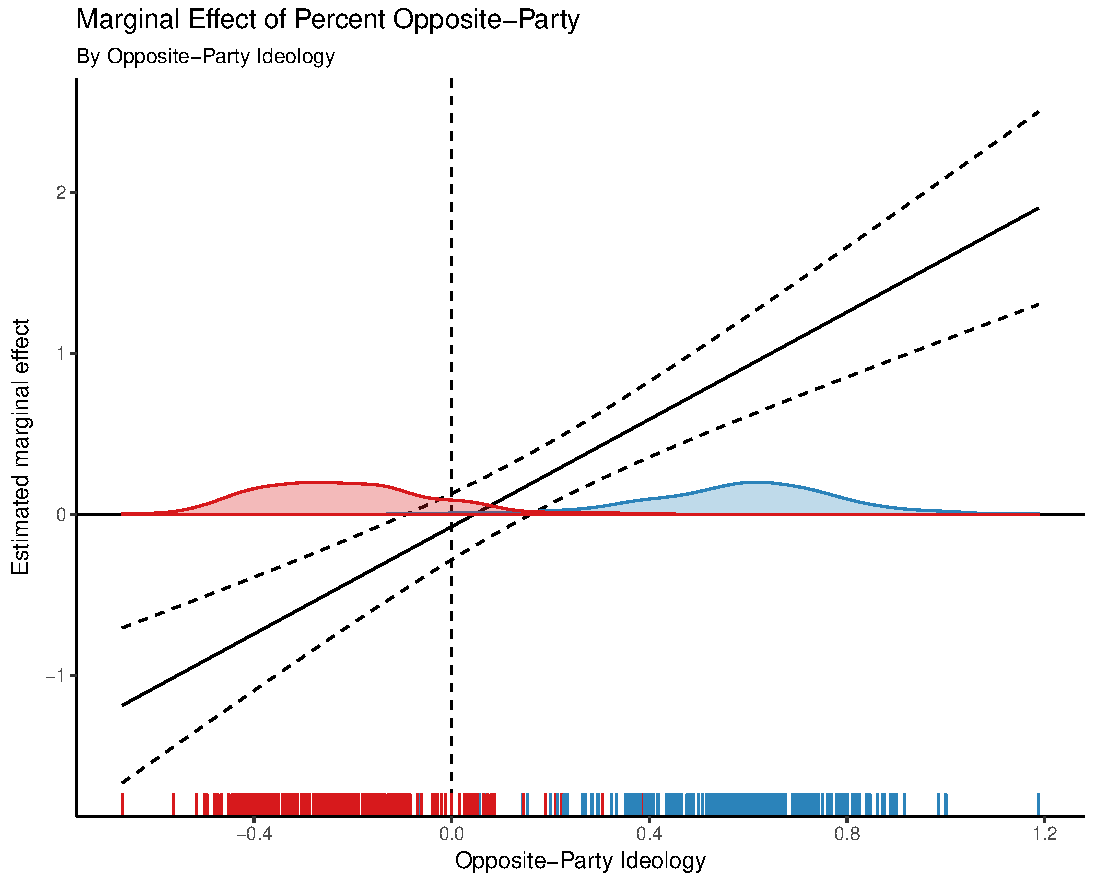
\includegraphics[width=.45\textwidth]{/Users/dsimp/GitHub/Clinton(2006)Rep/drafts/marginals/meb-5.pdf} &
    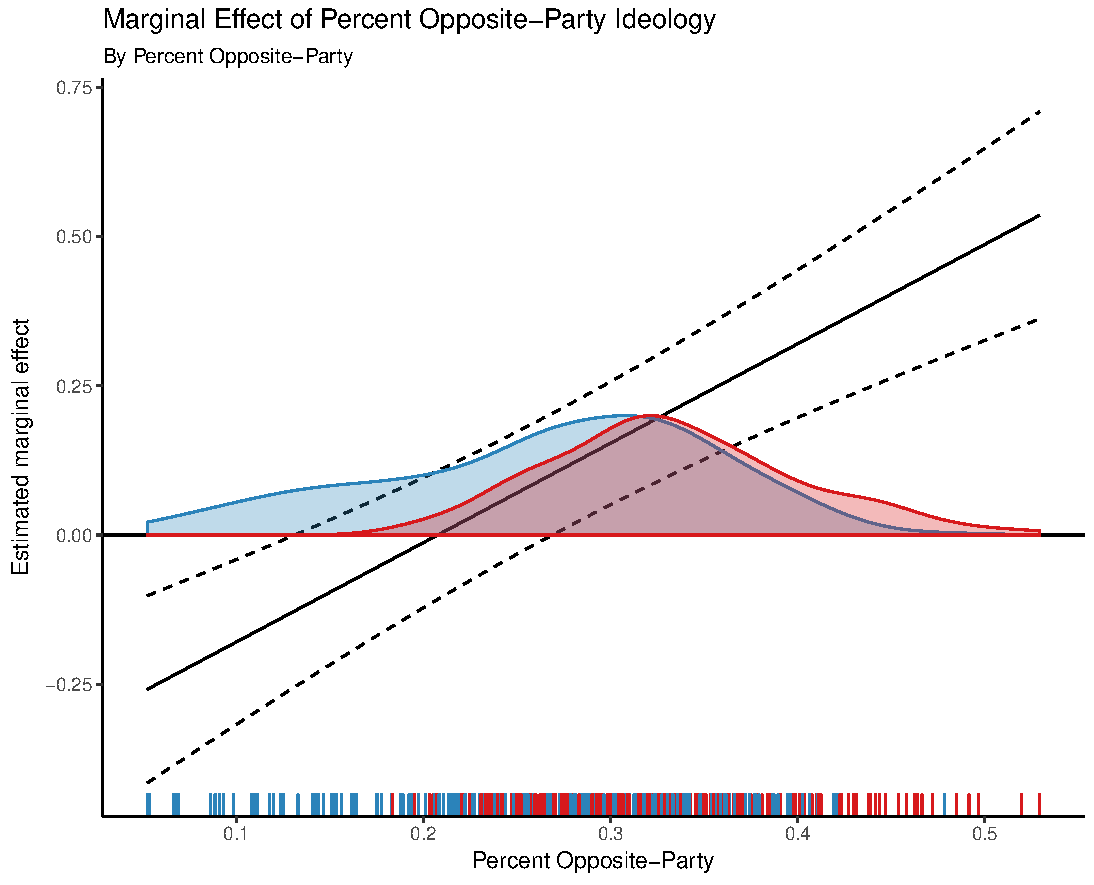
\includegraphics[width=.45\textwidth]{/Users/dsimp/GitHub/Clinton(2006)Rep/drafts/marginals/meb-6.pdf} \\
     &  \\
  \end{tabular}
    %}   
 \end{centering}
  \textbf{Note:} Each panel plots the respective marginal effect of the constitutive terms of the interaction variables in Table 2 Model 5.
\end{figure}
 

Clinton (2006) includes an errors in variable regression in the analysis following the practice of Gerald C. Wright, Robert S. Erikson and John P. McIver, and Fuller (1987).


\newpage

\subsection{Transformations and Interpretation}
A second, those less problematic, issue in the \cite{Clinton2006} analysis is the blah.

Often EIVreg is used when there is a low R-squared --> blah blah.

\newpage


\subsection{Ideology Scores}
To assess subconstituency influence on legislator behavior, \cite{Clinton2006} decomposes geographic constituency preferences into two weighted groups. The average ideology score $\bar{z}_i$ for each district $i$ is separated into the sample-population weighted same-party constituency preference $\frac{n_i^{SP}}{n_i}$ $\bar{z}_{SP_i}$ and the weighted nonsame-party constituency preference $\frac{n_i^{NSP}}{n_i}$ $\bar{z}_{NSP_i}$. The decomposition is shown in the below equation (3).

See equation (1):
\begin{equation}
\bar{z}_i = \bigg( \frac{n_i^{sp}}{n_i} \bigg) \bar{z}_{SP_i} + \bigg( \frac{n_i^{SP}}{n_i} \bigg) \bar{z}_{NSP_i}
\end{equation}
As stated above and shown in equation (1), \cite{Clinton2006} regresses legislator ideal points on the district party decomposition and a party indicator variable. Equation (2) and Table 1 models 2-4 demonstrate the problems with failing to include the constitutive variables of the interaction terms. However, the decomposition into two groups pose addition specification issues if independent voters are a large share of the non-same-party constituency and if these independent voters also voted for their district's current representative. 

\textit{However, such a specification can yield biased results if independent voters who are a large share of the nonsame-party constituency - especially if many independent voters also voted for their current representative.} \textbf{Figure 1, panel (I) demonstrates this potential problem. In Democratic districts, independent voters span the range -0.50 to 0.50, yet the same district opposite party voters are on average more conservative, with most scores falling between 0 and 1.2.} Similarly, in Republican districts independent voters are more conservative, with \textbf{Insert the comparison.} As such, it should be expected that legislators are sensitive to opinions of independent voters especially \textbf{when words}.

There is reason to expect this given democratic legislators span the spectrum of district ideology scores (See the below figure X). As such, decomposing district ideology scores into weighted same-party, weighted independent voters $\frac{n_i^{I}}{n_i}$ $\bar{z}_{I_i}$, and weighted opposite-party $\frac{n_i^{OP}}{n_i}$ $\bar{z}_{OP_i}$ will address this issue. The new specification is shown in equation (3).
\begin{equation}
y_i  = \beta_0 + \beta_1 \bigg( \frac{n_i^{SP}}{n_i} \bigg) \bar{z}_{SP_i} + \beta_3 \bigg( \frac{n_i^{I}}{n_i} \bigg) \bar{z}_{I_i} + \beta_4 \bigg( \frac{n_i^{OP}}{n_i} \bigg) \bar{z}_{OP_i} + \gamma I_{GOP} + \varepsilon_i
\end{equation}

\textbf{Do a marginal effects figure for same-party and non-same party as well. This can be used to show why the findings in Clinton (2006) are wrong.}

\newpage
\begin{figure}[!htbp]
\caption{District Group and Legislator Vote Distribution (All Votes)}
\begin{centering}
%\centering
%\fbox{
  \begin{tabular}{c}%{@{}ccc@{}}
    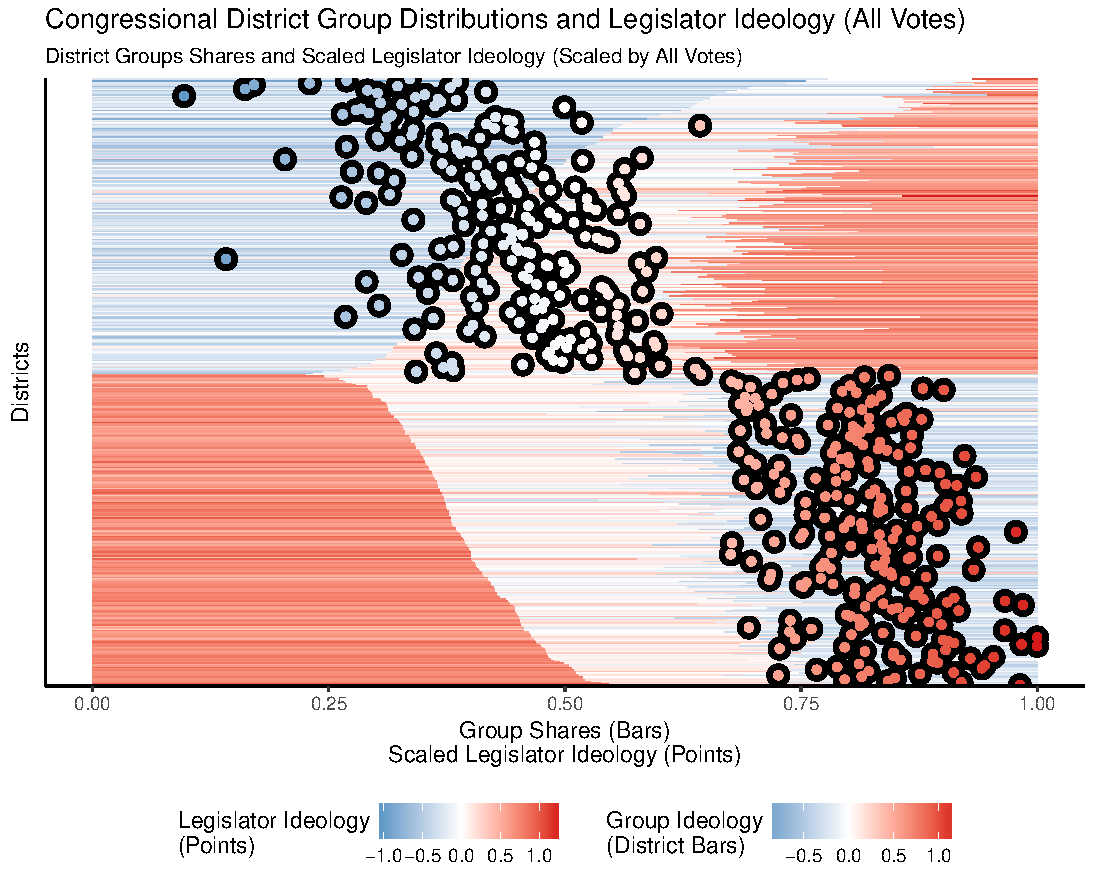
\includegraphics[width=.80\textwidth]{/Users/dsimp/GitHub/Clinton(2006)Rep/drafts/compare/compare1}\\
    \\
    \\
    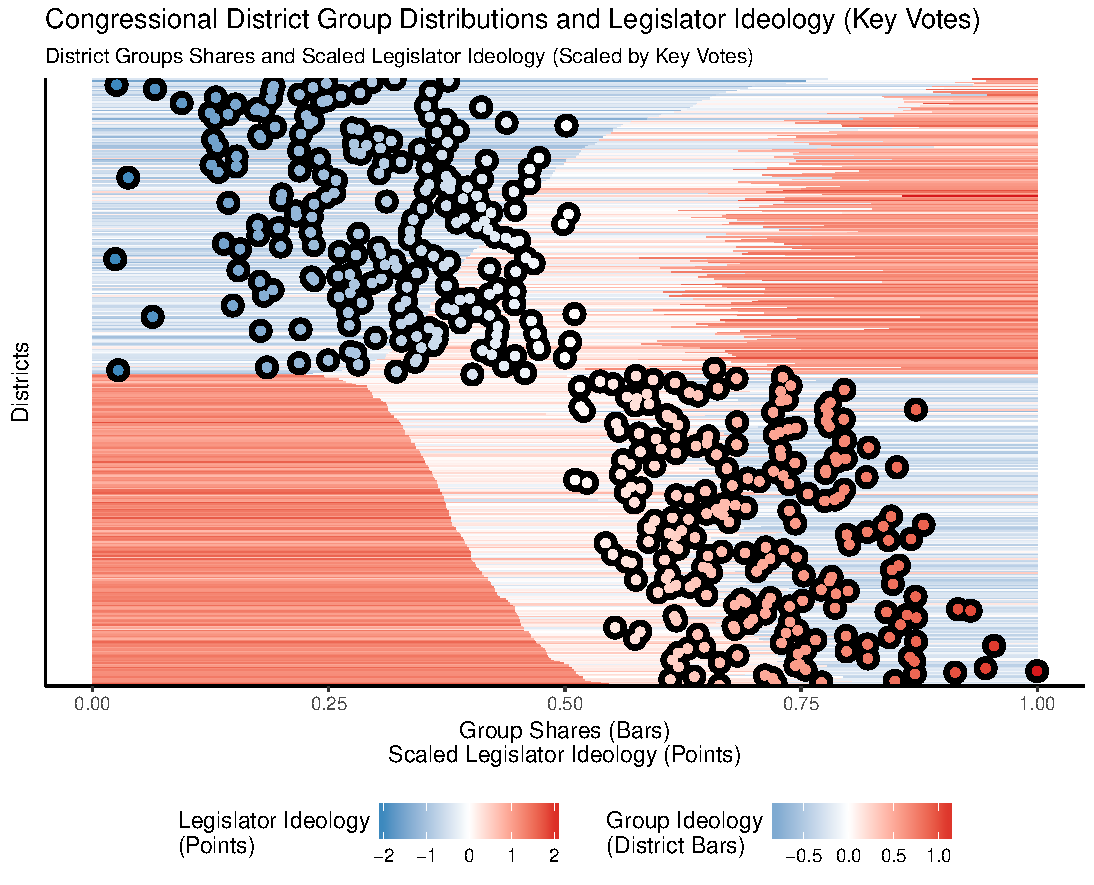
\includegraphics[width=.80\textwidth]{/Users/dsimp/GitHub/Clinton(2006)Rep/drafts/compare/compare2}\\
    %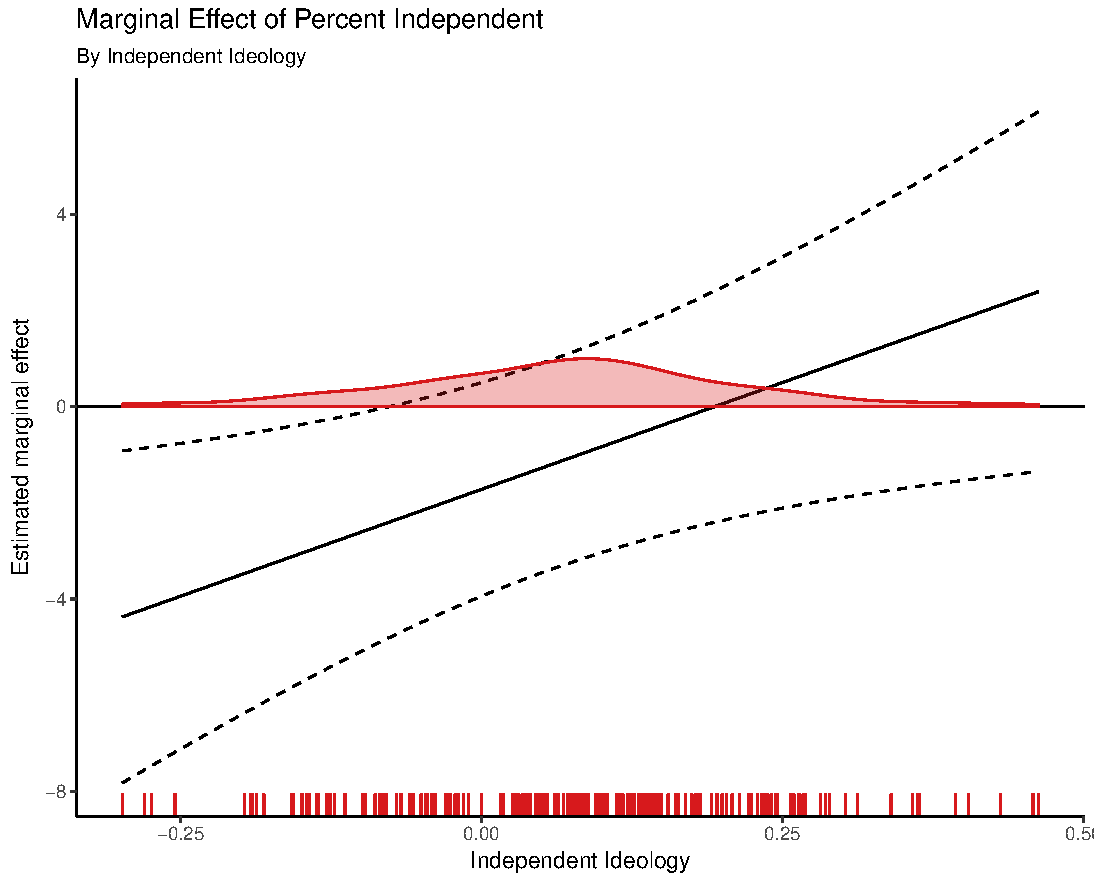
\includegraphics[width=.25\textwidth]{/Users/dsimp/GitHub/Clinton(2006)Rep/drafts/marginals/me4-3}
  \end{tabular}
    %}   
 \end{centering}\\
  %\textbf{Note:} Words 
\end{figure}

\newpage

\newpage

\newpage


\input{/Users/dsimp/GitHub/Clinton(2006)Rep/drafts/stargazer/table3.txt}

% Interaction Terms All Votes
\begin{figure}[!htbp]
\caption{Marginal Effects of Interaction Terms (All Votes)}
\begin{centering}
%\centering
%\fbox{
  \begin{tabular}{ccc}%{@{}ccc@{}}
	& \small \textbf{GOP Regression} & \\ 
	& & \\ 	
  	\small (A) Percent Same-Party& 
  	\small (B) Percent Independent& 
    \small (C) Percent Opposite-Party\\
    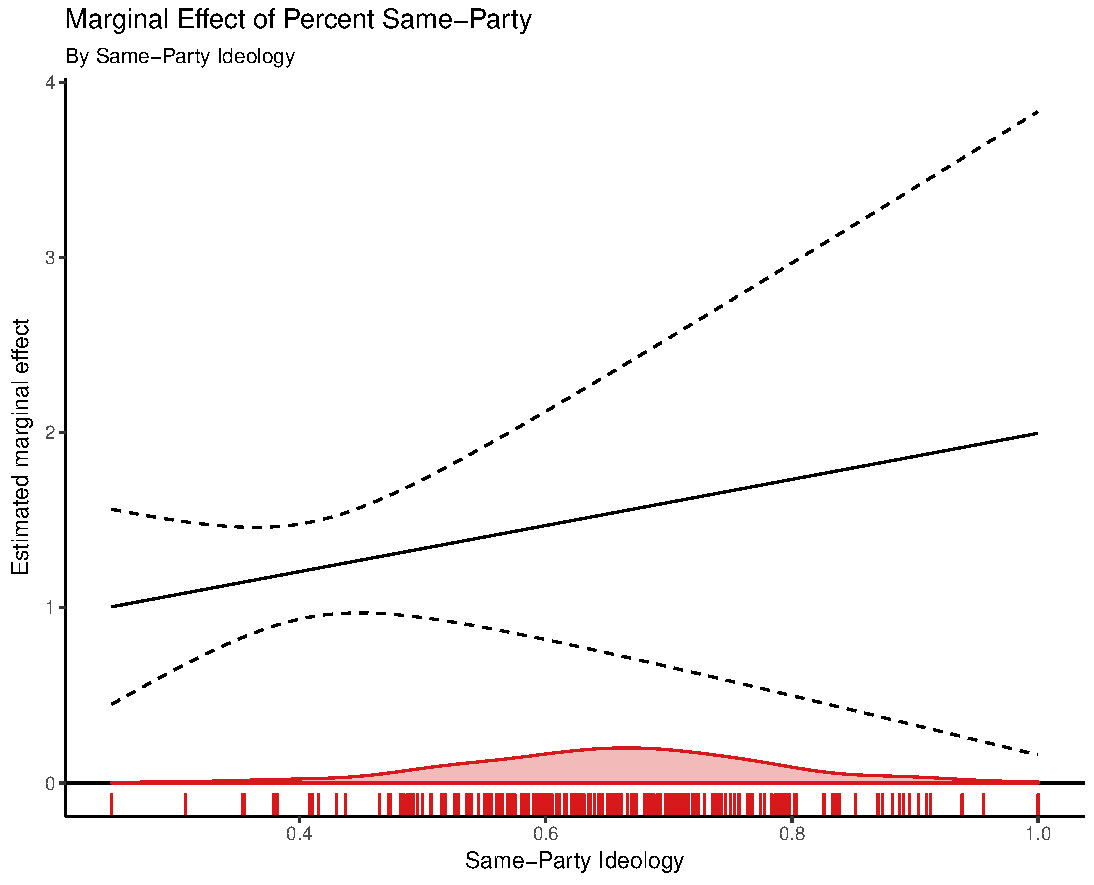
\includegraphics[width=.25\textwidth]{/Users/dsimp/GitHub/Clinton(2006)Rep/drafts/marginals/me2-1} &
    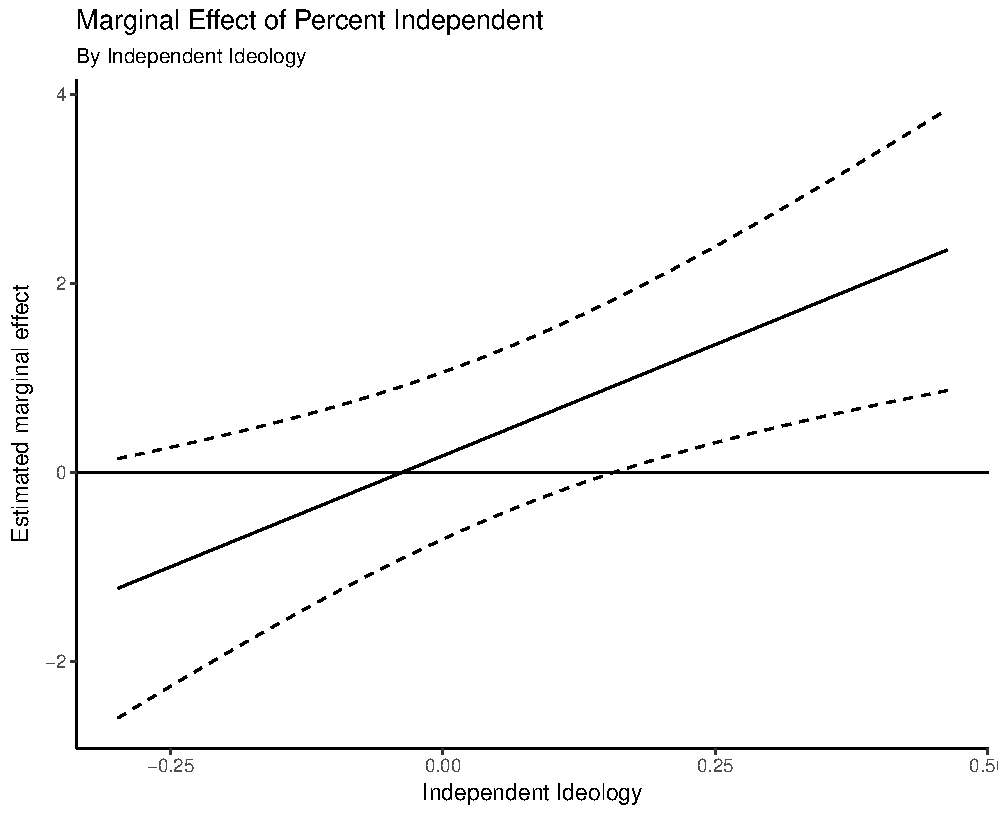
\includegraphics[width=.25\textwidth]{/Users/dsimp/GitHub/Clinton(2006)Rep/drafts/marginals/me2-3} &
    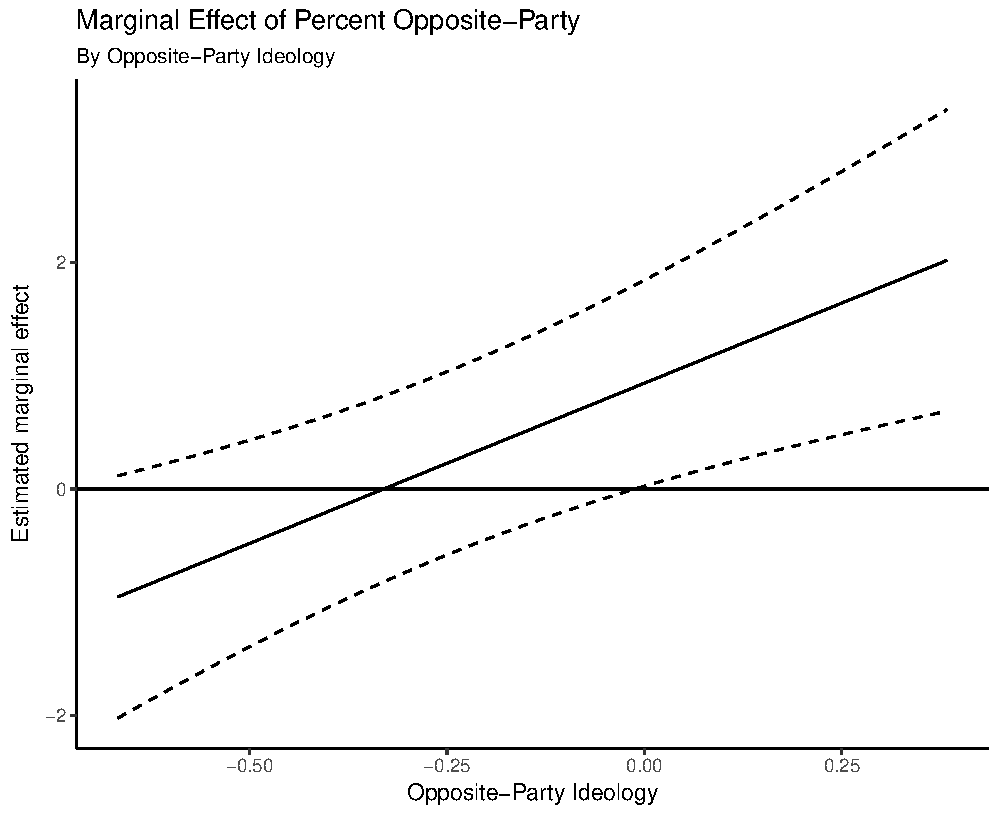
\includegraphics[width=.25\textwidth]{/Users/dsimp/GitHub/Clinton(2006)Rep/drafts/marginals/me2-5} \\
     & & \\
  	\small (D) Same-Party Ideology& 
  	\small (E) Independent& 
    \small (F) Opposite-Party Ideology\\
    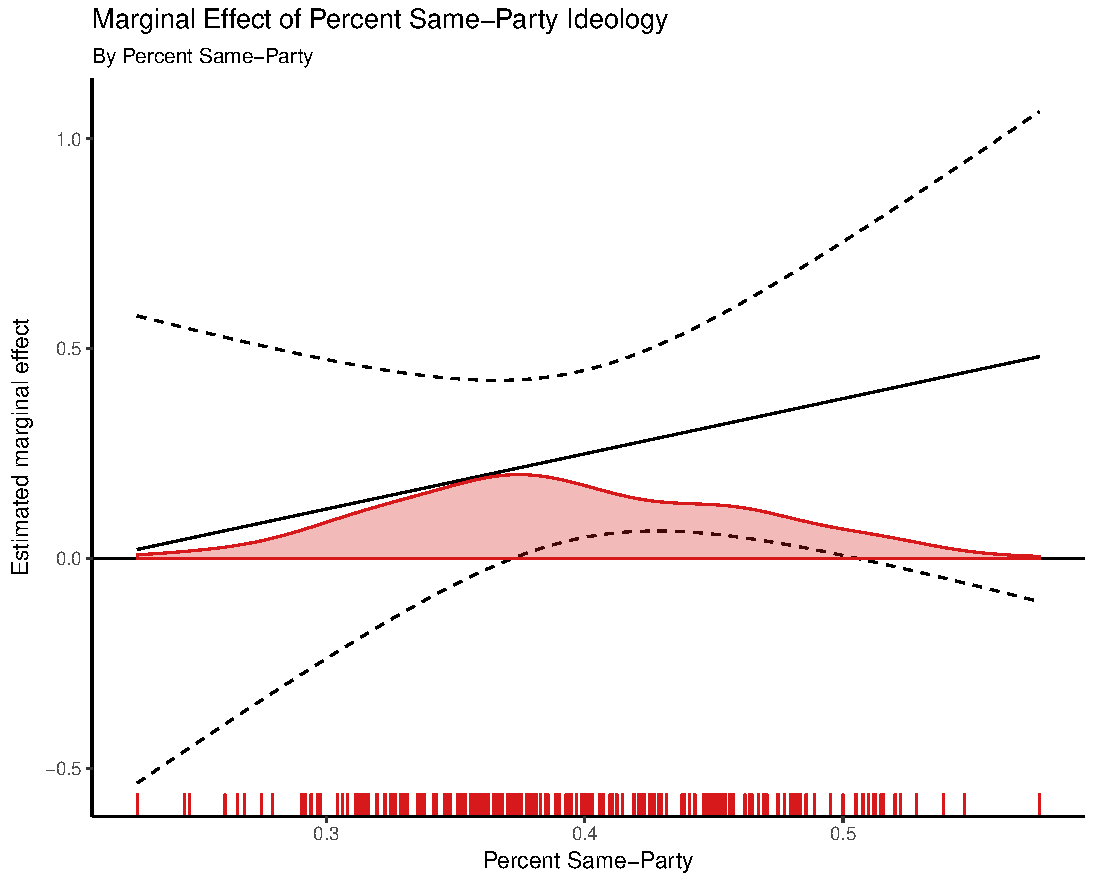
\includegraphics[width=.25\textwidth]{/Users/dsimp/GitHub/Clinton(2006)Rep/drafts/marginals/me2-2} &
    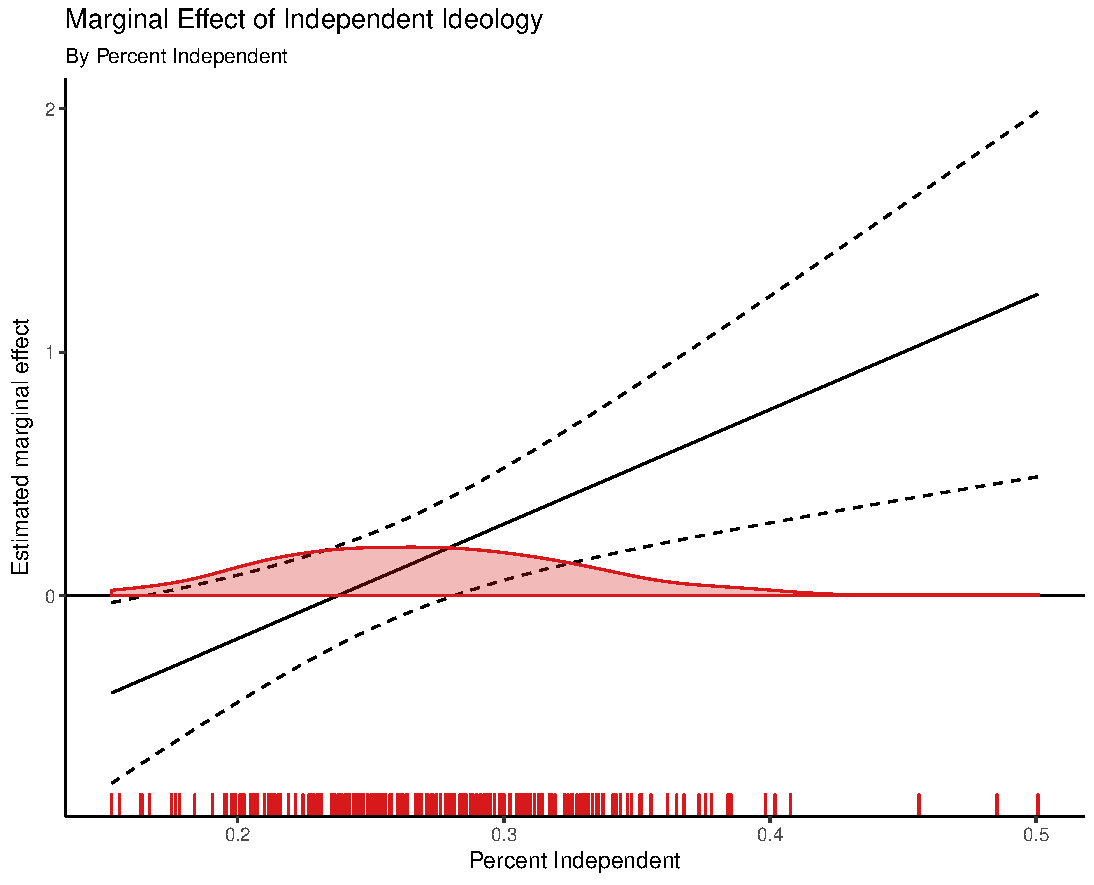
\includegraphics[width=.25\textwidth]{/Users/dsimp/GitHub/Clinton(2006)Rep/drafts/marginals/me2-4} &
    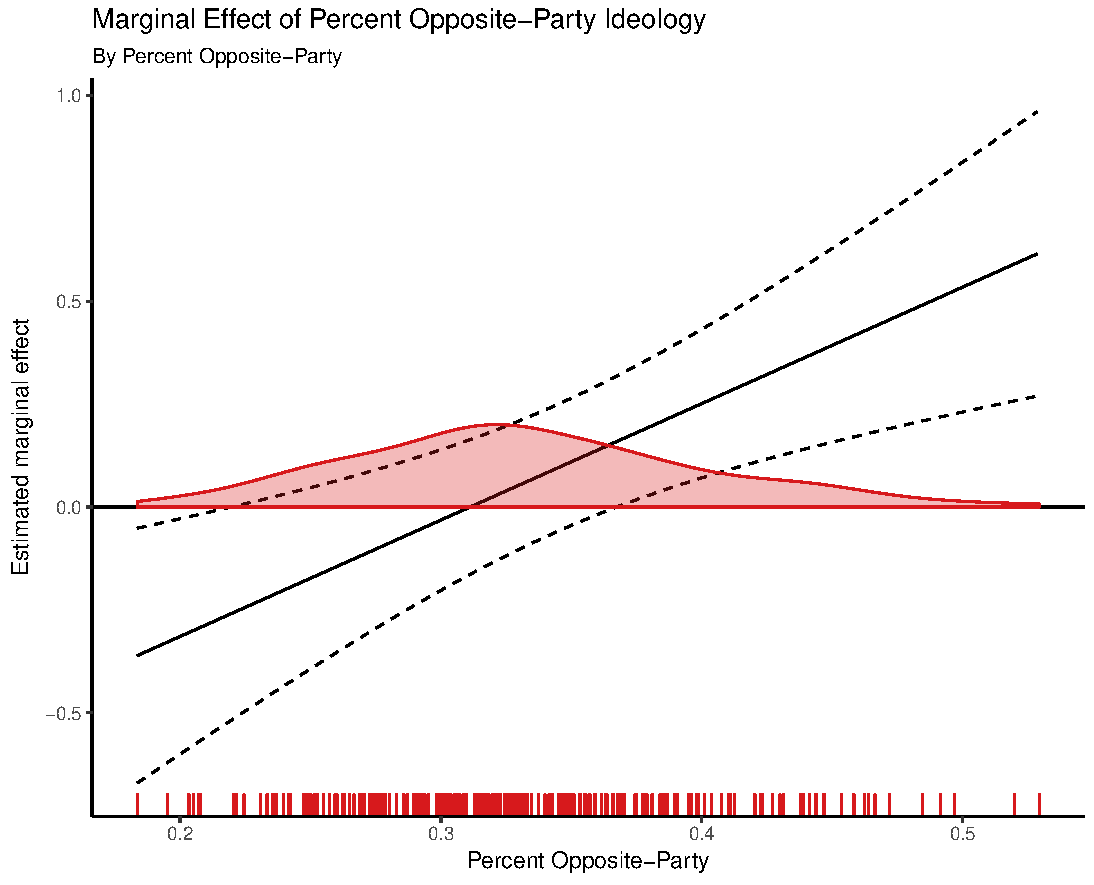
\includegraphics[width=.25\textwidth]{/Users/dsimp/GitHub/Clinton(2006)Rep/drafts/marginals/me2-6} \\
    	& & \\ 
	& \small \textbf{DEM Regression} & \\ 
	& & \\ 
  	\small (G) Percent Same-Party& 
  	\small (H) Percent Independent& 
    \small (I) Percent Opposite-Party\\
    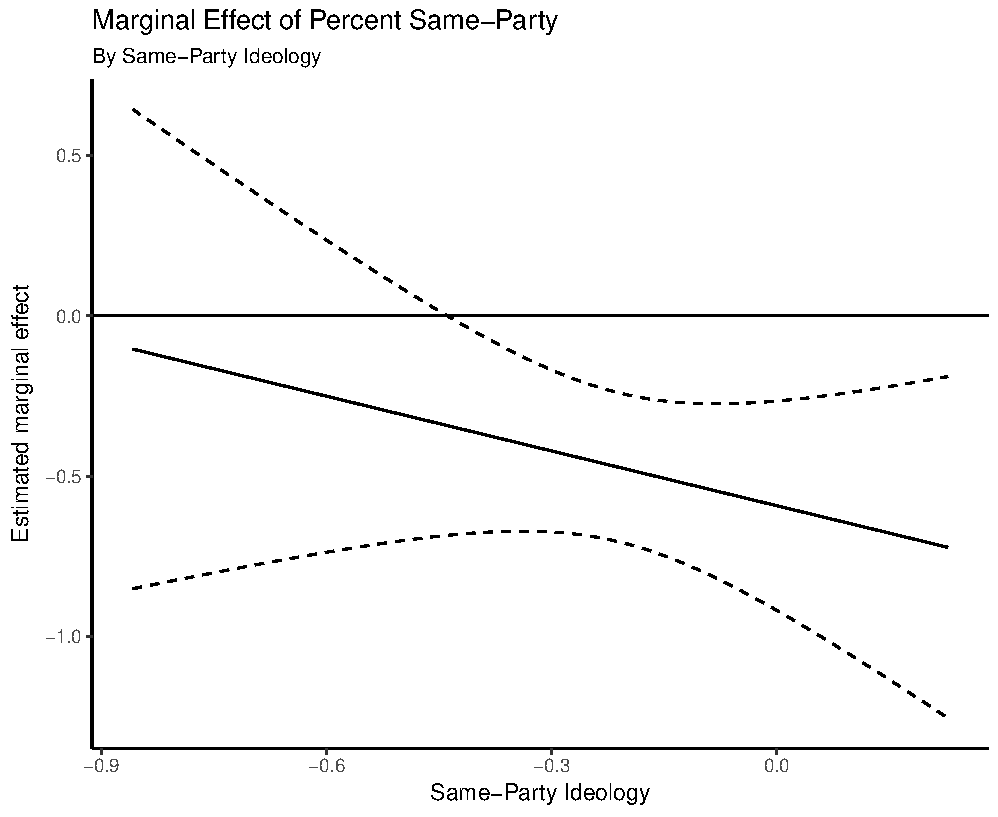
\includegraphics[width=.25\textwidth]{/Users/dsimp/GitHub/Clinton(2006)Rep/drafts/marginals/me3-1} &
    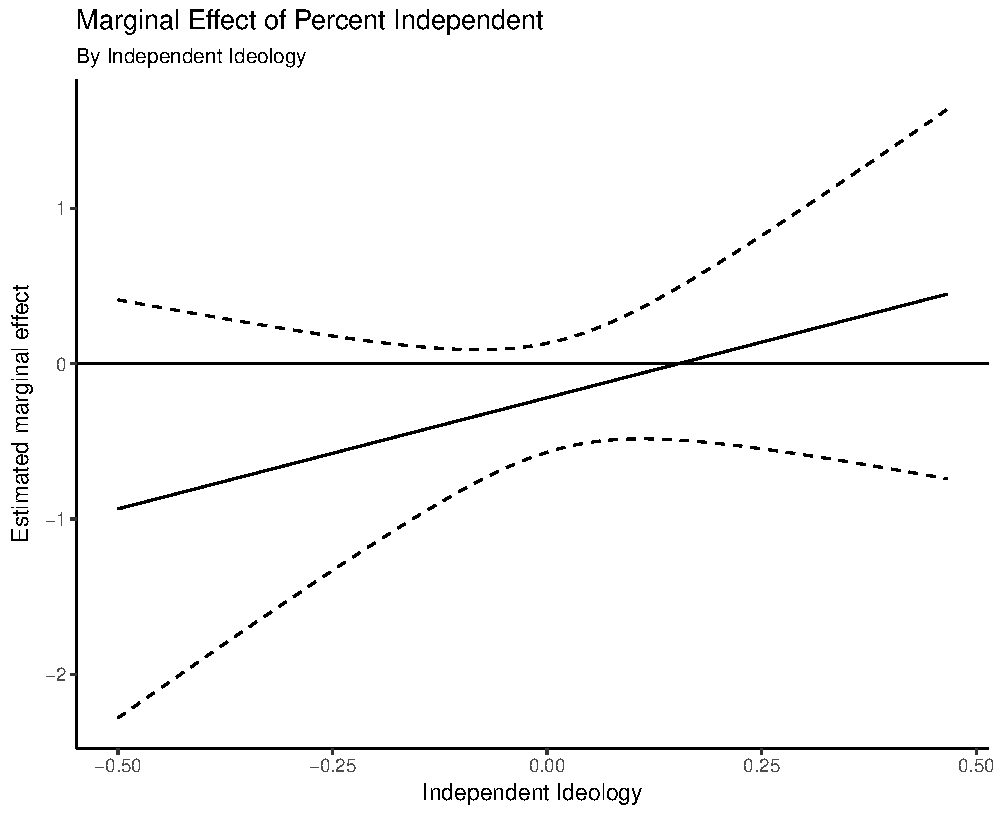
\includegraphics[width=.25\textwidth]{/Users/dsimp/GitHub/Clinton(2006)Rep/drafts/marginals/me3-3} &
    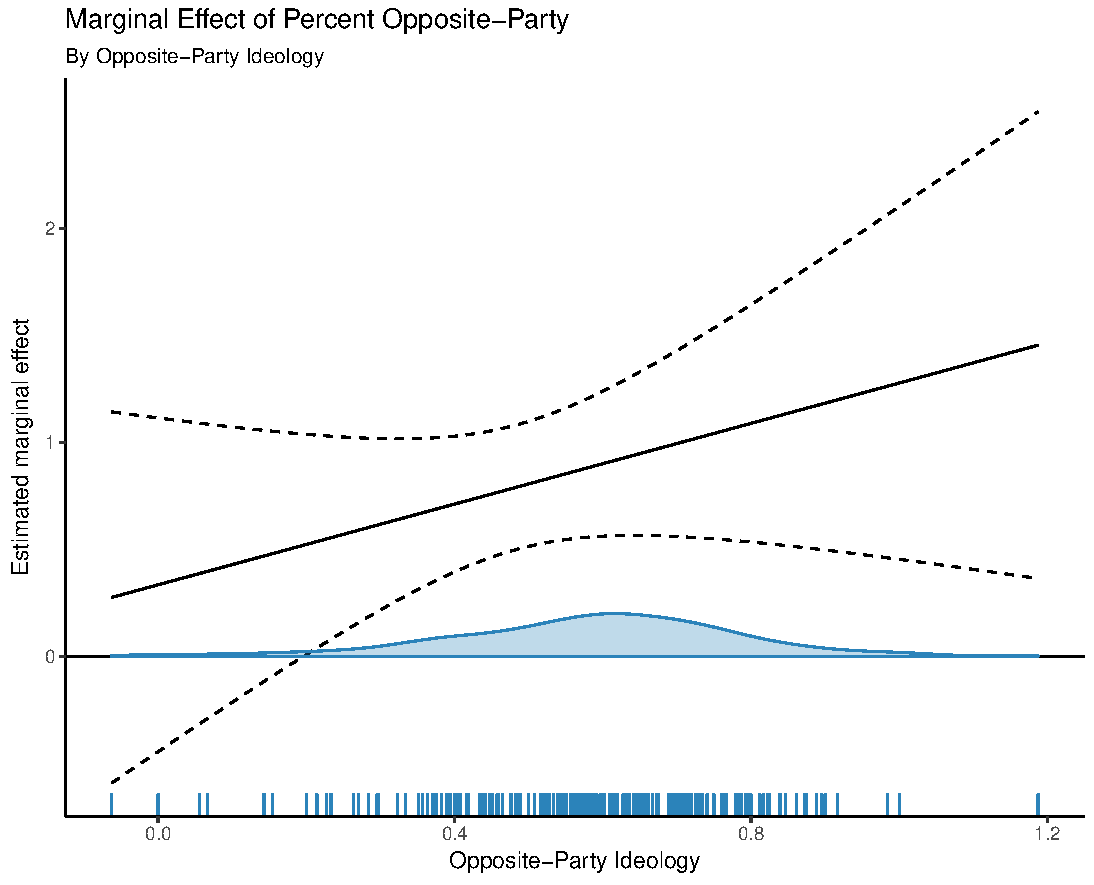
\includegraphics[width=.25\textwidth]{/Users/dsimp/GitHub/Clinton(2006)Rep/drafts/marginals/me3-5} \\
     & & \\
  	\small (J) Same-Party Ideology& 
  	\small (K) Independent Ideology& 
    \small (H) Opposite-Party Ideology\\
    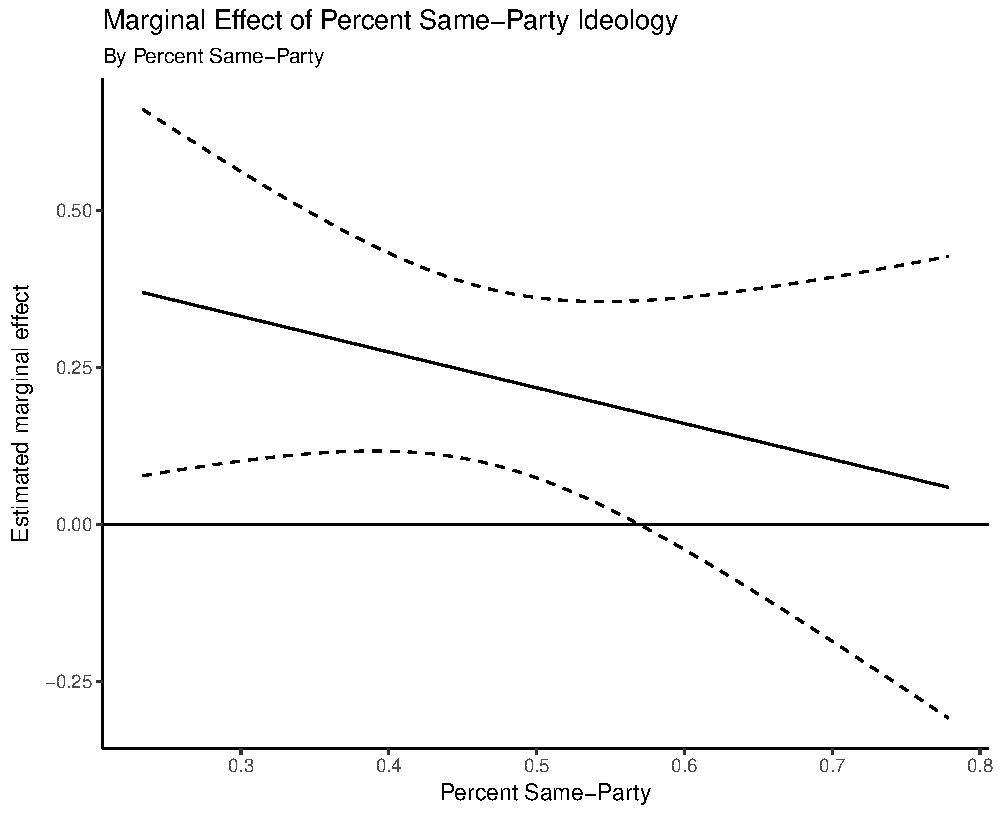
\includegraphics[width=.25\textwidth]{/Users/dsimp/GitHub/Clinton(2006)Rep/drafts/marginals/me3-2} &
    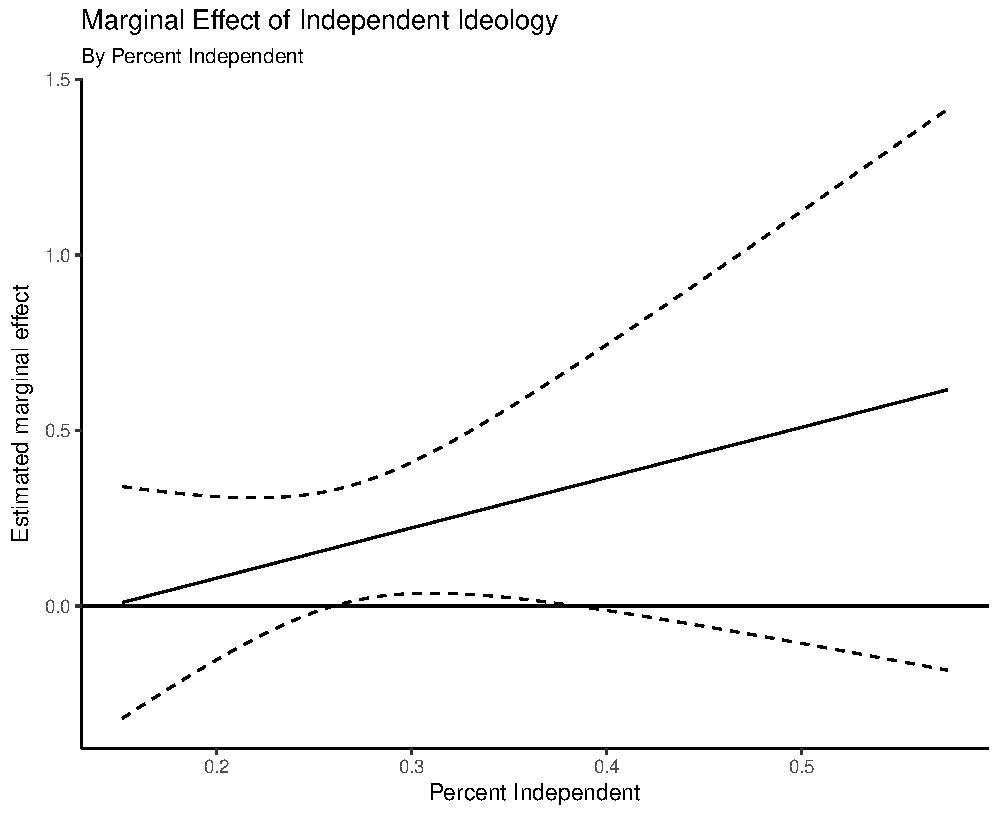
\includegraphics[width=.25\textwidth]{/Users/dsimp/GitHub/Clinton(2006)Rep/drafts/marginals/me3-4} &
    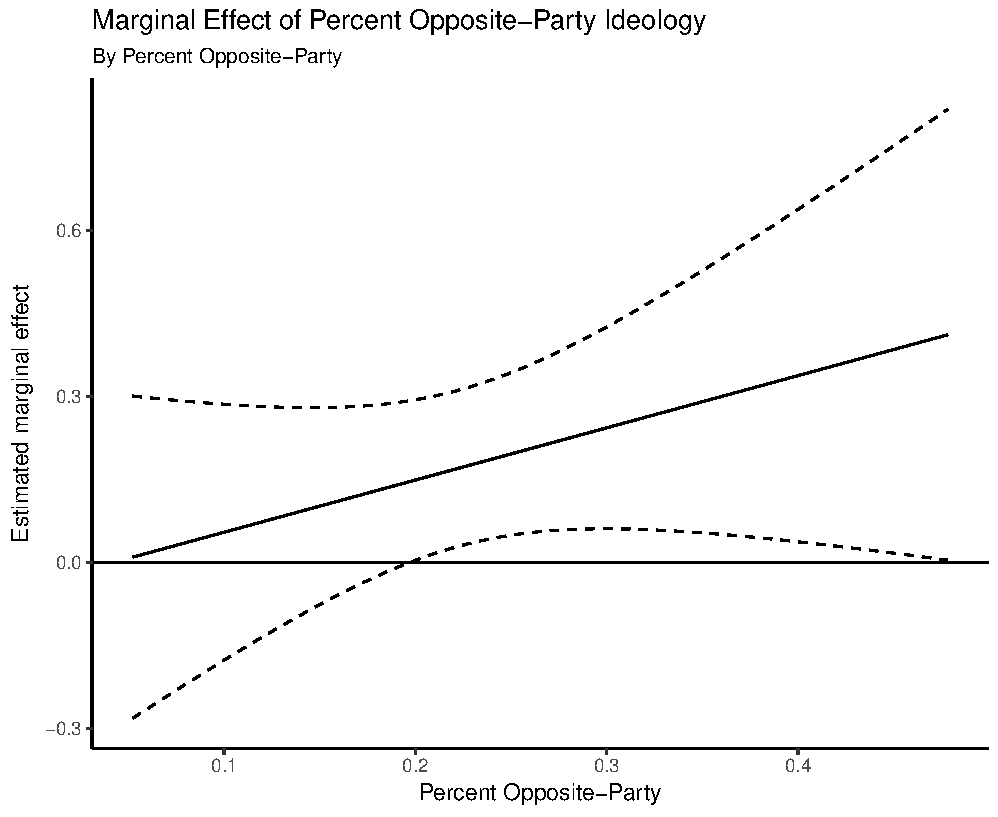
\includegraphics[width=.25\textwidth]{/Users/dsimp/GitHub/Clinton(2006)Rep/drafts/marginals/me3-6} \\
     & & \\
  \end{tabular}
    %}   
 \end{centering}\\
  \textbf{Note:} . 
\end{figure}
 

\newpage

\subsection{Delegate Paradox}


To first explore the Delegate Paradox, I plan to consider the relationship between district ideology and legislator ideal points using all votes in the 106th House and then key votes in the 106th House. Clinton provides both of these measures in the replication data. Observe Table 1, Representative ideal points have a smaller mean and a larger standard deviation when measured using key votes rather than all votes. I then plan to consider the relationship between district ideology and legislator behavior on individual bills using a probit model.

To further explore the Delegate Paradox, I plan to compare the voting behavior of different party legislators with similar district ideologies. I then plan to compare the voting behavior of legislators who won in close elections using election data from the 1998 Midterm election.

Long term, I plan to employ MRP and consider the voting behavior of legislator using survey data related to key votes in the 106th House.

\newpage

\input{/Users/dsimp/GitHub/Clinton(2006)Rep/drafts/stargazer/table4.txt}


% Interaction Terms Key Votes
\begin{figure}[!htbp]
\caption{Marginal Effects of Interaction Terms (Key Votes)}
\begin{centering}
%\centering
%\fbox{
  \begin{tabular}{ccc}%{@{}ccc@{}}
	& \small \textbf{GOP Regression} & \\ 
	& & \\ 	
  	\small (A) Percent Same-Party& 
  	\small (B) Percent Independent& 
    \small (C) Percent Opposite-Party\\
    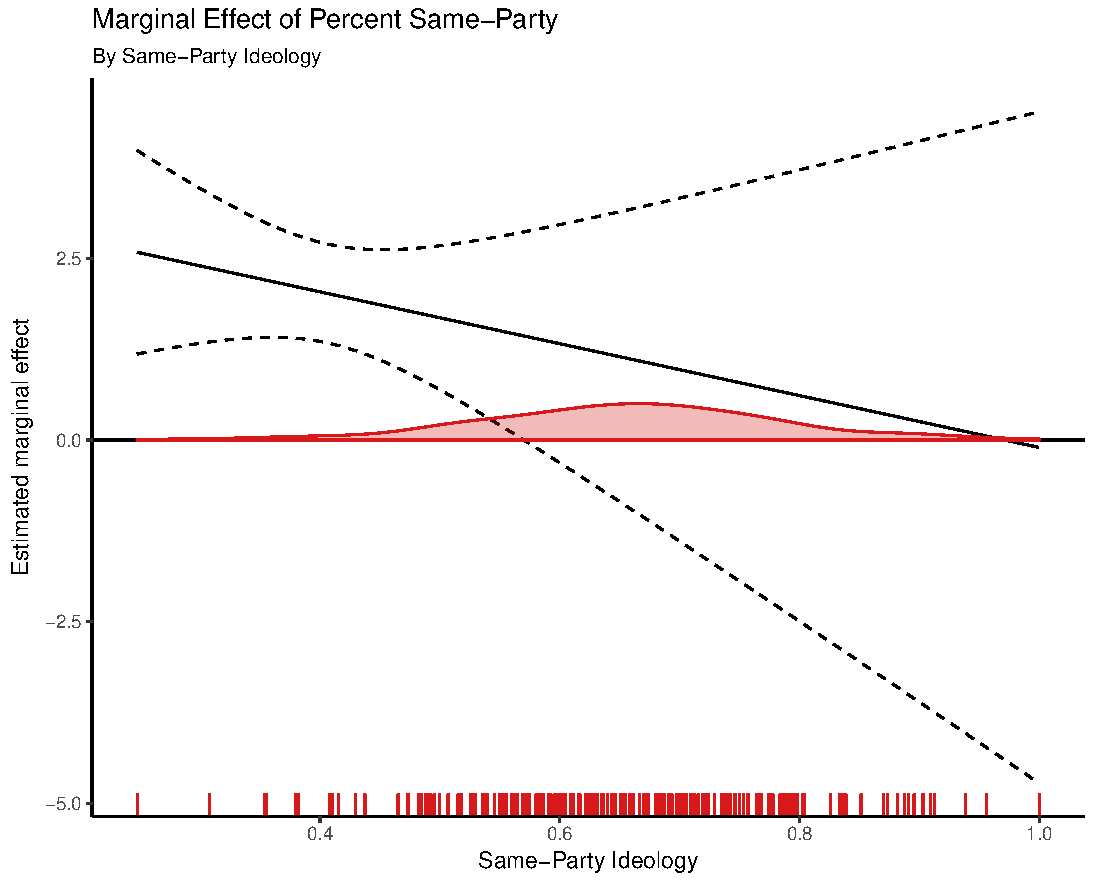
\includegraphics[width=.25\textwidth]{/Users/dsimp/GitHub/Clinton(2006)Rep/drafts/marginals/me4-1} &
    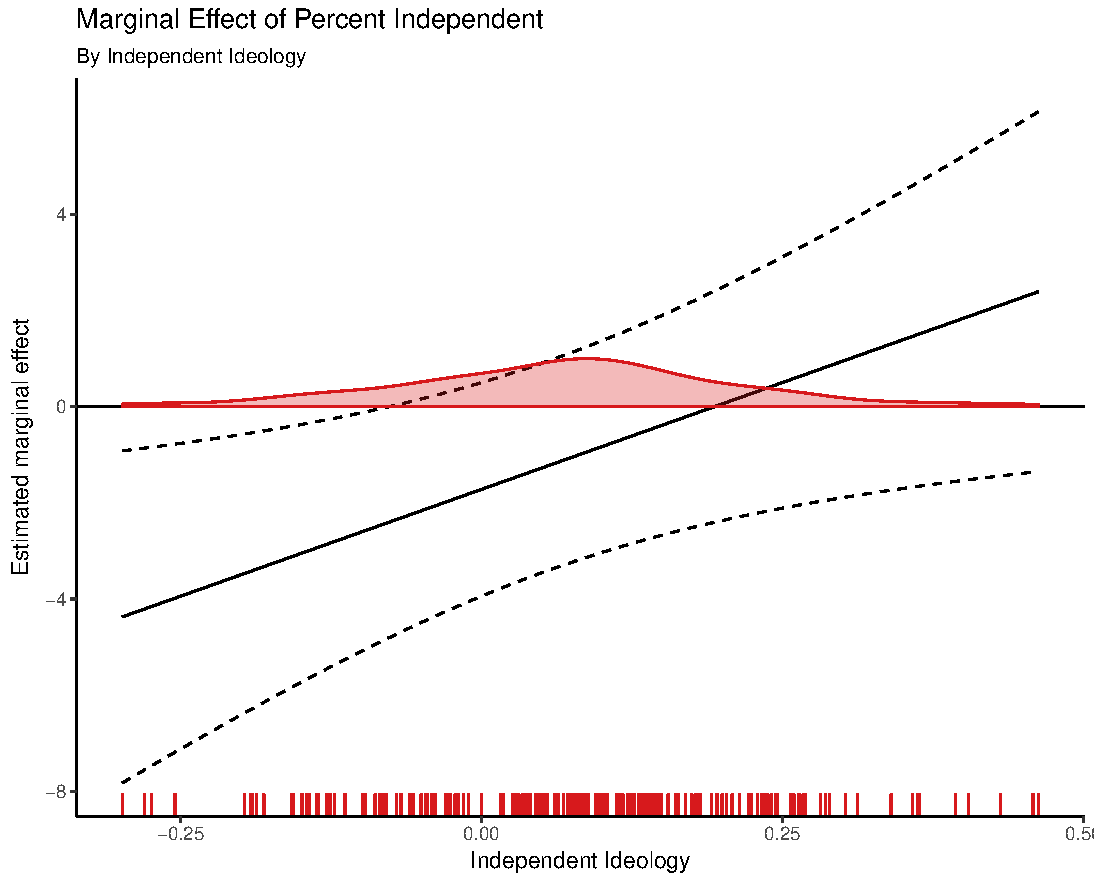
\includegraphics[width=.25\textwidth]{/Users/dsimp/GitHub/Clinton(2006)Rep/drafts/marginals/me4-3} &
    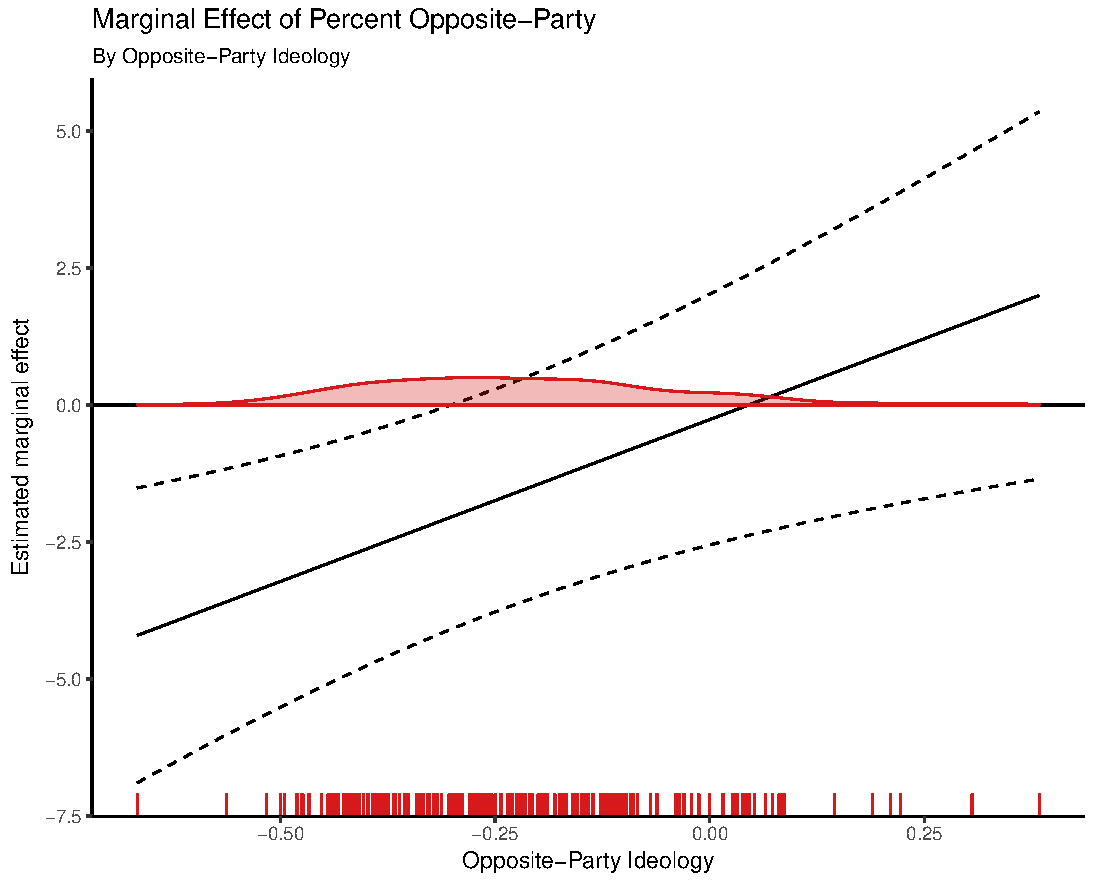
\includegraphics[width=.25\textwidth]{/Users/dsimp/GitHub/Clinton(2006)Rep/drafts/marginals/me4-5} \\
     & & \\
  	\small (D) Same-Party Ideology& 
  	\small (E) Independent Ideology& 
    \small (F) Opposite-Party Ideology\\
    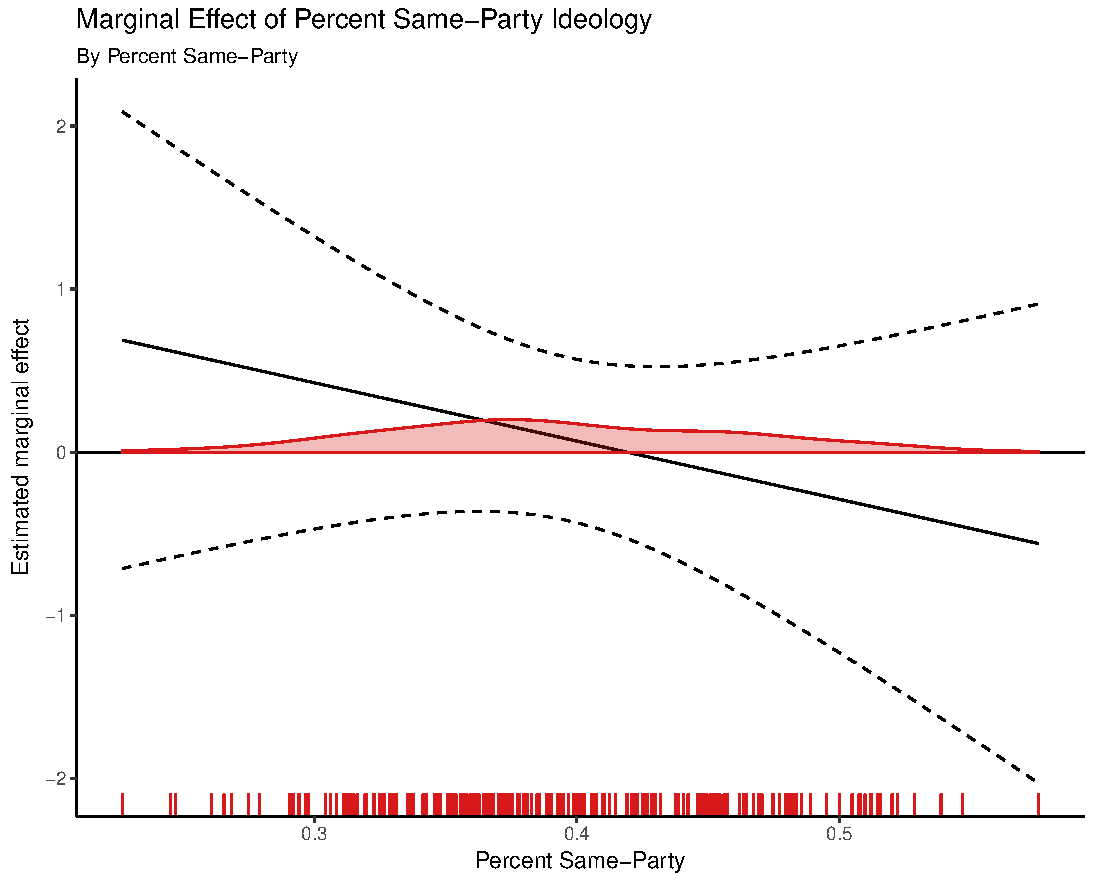
\includegraphics[width=.25\textwidth]{/Users/dsimp/GitHub/Clinton(2006)Rep/drafts/marginals/me4-2} &
    \includegraphics[width=.25\textwidth]{/Users/dsimp/GitHub/Clinton(2006)Rep/drafts/marginals/me4-4} &
    \includegraphics[width=.25\textwidth]{/Users/dsimp/GitHub/Clinton(2006)Rep/drafts/marginals/me4-6} \\
    	& & \\ 
	& \small \textbf{DEM Regression} & \\ 
	& & \\ 
  	\small (G) Percent Same-Party& 
  	\small (H) Percent Independent&  
    \small (I) Percent Opposite-Party\\
    \includegraphics[width=.25\textwidth]{/Users/dsimp/GitHub/Clinton(2006)Rep/drafts/marginals/me5-1} &
    \includegraphics[width=.25\textwidth]{/Users/dsimp/GitHub/Clinton(2006)Rep/drafts/marginals/me5-3} &
    \includegraphics[width=.25\textwidth]{/Users/dsimp/GitHub/Clinton(2006)Rep/drafts/marginals/me5-5} \\
     & & \\
  	\small (J) Same-Party Ideology& 
  	\small (K) Independent Ideology& 
    \small (H) Opposite-Party Ideology\\
    \includegraphics[width=.25\textwidth]{/Users/dsimp/GitHub/Clinton(2006)Rep/drafts/marginals/me5-2} &
    \includegraphics[width=.25\textwidth]{/Users/dsimp/GitHub/Clinton(2006)Rep/drafts/marginals/me5-4} &
    \includegraphics[width=.25\textwidth]{/Users/dsimp/GitHub/Clinton(2006)Rep/drafts/marginals/me5-6} \\
     & & \\
  \end{tabular}
    %}   
 \end{centering}\\
  \textbf{Note:} . 
\end{figure}
 

% 


\newpage


\subsection{Non-Common Scale}
To consider the Non-Common Scales issue I propose running the equation (3) specification using two additional methods for generating ideology scores \textbf{DW-Nominate}, and \textbf{CF-Scores}. Though all three measures are correlated, this procedure will explore how different measures affect the slope between district opinion ideology and legislator ideal points. Furthermore, it will demonstrate why the Non-Common Scale problem implies that the slope and intercept of the responsiveness curve lack direct meanings.The representative ideal points in Clinton (2006) were generated using a methodology described in Clinton (2004).


I have reproduced Clinton (2009) Figure 1. Below it is followed by replication results from Clinton (2009) Table 1 and Table 2. In each table I have reproduced Clinton's OLS findings and also included replication regression where I use Same-Party Ideology, Independent Ideology and Opposite Party Ideology.





\section{Discussion} 







\newpage
%\input{/Users/dsimp/GitHub/Clinton(2006)Rep/drafts/table3.txt}

\newpage


\newpage

\newpage


\section{Conclusion} 
This paper has demonstrated that independent voters cannot be lumped with opposite party voters when studying the relationship between legislator voting behavior and sub-district constituent ideology. It also explore the sensitivity of various forms of ideology measures.

Future extensions of this project include comparing the stability of the results with other measures of legislator ideal points as well as to employ MRP for individual topic analysis.

Possible extensions to this project include a more in depth analysis of the Non-Common scale issue. Potential datasets include DW-Nominate Scores as well as CF-Scores. Such analysis would further tease out the consistency of using legislator votes to measure the relationship between behavior and sub-district ideology.

Another extension could consider using survey data. I would plan to identify data relevant to key votes in the 106th House. I would then use MRP to consider the relationship between voter preferences and outcomes on kev votes by topic. This would allow me to compare legislator responsiveness to district ideology to legislator responsiveness to district issue preferences.


A longer term extension of this project would be to 

Election Results data to explore the behavior of legislators who won close elections.
Census data - to explore how legislator ideal points varies with district ideology and district demographic characteristics. 

\section{Next Steps} 

This section includes next steps and ideas for the next draft of this paper.

\textbf{Cosmetic Next Steps}
\begin{itemize}
\item Include an appendix table of the 106th House Key Votes.
\item Change the arrangement of the panels in Figure 3. Vertically align the marginal effects of party share and party ideology instead of vertically align.
\item Add a model 5 to Table 2 that includes all three groups (SP ,IND, and OP) in the regression.
\item Also, add an additional figure to demonstrate the marginal effects plots of the new model 5.
\end{itemize}

\textbf{Include}
\begin{itemize}
\item Include a model of three groups
\item \textit{Competitiveness:} I could explore whether the difference between signaled and revealed preference (all vs key vote difference) is correlated with the size of a legislators election victory. Though victory size is also likely endogenously related to district competitiveness.
\item \textit{Presidential Vote Share"} I could explore whether the 
all vs key vote difference is correlated districts with the percentage of Clinton voters in 1994 or Gore voters in 2000 
\end{itemize}

\textbf{Sensitivity Analysis}
\begin{itemize}
\item Explore the impact of different weight matrices. Clinton weights his standard errors using the number of constituent respondents in each district. As such, he excludes the total number of sampled individuals in the district. That is he does not count individuals who did not answer the ideology preference question. 
\item Include an appendix table of the 106th House Key Votes.
\end{itemize}



\newpage

\newpage

\bibliography{citations}

\newpage
\section{Appendix} 
% Reset & Rename the Name Configuration of Tables and Figures
\setcounter{table}{0}
\renewcommand{\thetable}{A\arabic{table}}
\setcounter{figure}{0}
\renewcommand{\thefigure}{A\arabic{figure}}

% Ideal Points Summary Table
%\input{/Users/dsimp/GitHub/Clinton(2006)Rep/drafts/summary/summary1.txt}
Table A1 provides the summary statistics for Welch's t-tests of Republican and Democratic legislator ideal points. The absolute ideal point is found by taking the absolute value of all ideal points.
\input{/Users/dsimp/GitHub/Clinton(2006)Rep/drafts/summary/summarystat1.txt} 

Table A2 provides summary statistics for district ideology and sub-district ideology and percent share of total constituents. The statistics are grouped by legislator party. For example, the mean ideology of Democratic constituents in an average district with a Republican legislator is -0.219. The corresponding mean share of the total Democratic voters in an average district with a Republican legislator is 33.3\%.
\input{/Users/dsimp/GitHub/Clinton(2006)Rep/drafts/summary/summary2.txt} 


% Figure A1 is histograms of Group shares.
\begin{figure}[!htbp]
\caption{Distribution of District Group Shares}
\begin{centering}
%\centering
%\fbox{
  \begin{tabular}{@{}cc@{}}
	% & & \\  	
  	\small (A) Same-Party Share &
    \small (B) Non-Same-Party Share  \\
    \includegraphics[width=.45\textwidth]{/Users/dsimp/GitHub/Clinton(2006)Rep/drafts/histogram/histogram2-1.pdf} &
    \includegraphics[width=.45\textwidth]{/Users/dsimp/GitHub/Clinton(2006)Rep/drafts/histogram/histogram2-2.pdf} \\
    % & & \\
    \small (C) Opposite-Party Share & 
    \small (D) Independent Share\\
    \includegraphics[width=.45\textwidth]{/Users/dsimp/GitHub/Clinton(2006)Rep/drafts/histogram/histogram2-3.pdf} &
    \includegraphics[width=.45\textwidth]{/Users/dsimp/GitHub/Clinton(2006)Rep/drafts/histogram/histogram2-4.pdf} \\
    % &  &\\
  \end{tabular}
    %}   
 \end{centering}
 \small~~~~~~~~\textbf{Note:} The histograms illustrate the distribution of constituency group share of total district voters. Districts are classified by the party of their legislator. The short dashed lines are the Republican controlled district means, the long dashed line are the Democratic controlled district means, and the dotted and dashed line is the chamber mean.
\end{figure}. 

% Figure A2 is Ideal Point and Group share plots.
\begin{figure}[!htbp]
\caption{Legislator Ideal Points and District Ideology Means}
\begin{centering}
%\centering
%\fbox{
  \begin{tabular}{@{}cc@{}}
	% & & \\  	
  	\small (A) Ideal Point &
    \small (B) Ideal Point  \\
    \small vs Same-Party Share & 
    \small vs Non-Same-Party Share\\
    \includegraphics[width=.45\textwidth]{/Users/dsimp/GitHub/Clinton(2006)Rep/drafts/plots/shareplot1.pdf} &
    \includegraphics[width=.45\textwidth]{/Users/dsimp/GitHub/Clinton(2006)Rep/drafts/plots/shareplot2.pdf} \\
    % & & \\
    \small (C) Ideal Point & 
    \small (D) Same-Party Ideology\\
    \small vs Opposite Party Share  & 
    \small vs Independent Share\\
    \includegraphics[width=.45\textwidth]{/Users/dsimp/GitHub/Clinton(2006)Rep/drafts/plots/shareplot3.pdf} &
    \includegraphics[width=.45\textwidth]{/Users/dsimp/GitHub/Clinton(2006)Rep/drafts/plots/shareplot4.pdf} \\
    % &  &\\
  \end{tabular}
    %}   
 \end{centering}
 \small~~~~~~~~\textbf{Note:} Districts represented by Republicans (Democrats) are plotted with triangles (circles). A bivariate trend line is plotted for overall comparison and party trend lines are plotted for comparison within districts.
\end{figure}. 

% Figure A3 is Key Ideal Point and Group share plots.
%\begin{figure}[!htbp]
\caption{Legislator Ideal Points and District Ideology Means}
\begin{centering}
%\centering
%\fbox{
  \begin{tabular}{@{}cc@{}}
	% & & \\  	
  	\small (A) Ideal Point &
    \small (B) Ideal Point  \\
    \small vs Same-Party Share & 
    \small vs Non-Same-Party Share\\
    \includegraphics[width=.45\textwidth]{/Users/dsimp/GitHub/Clinton(2006)Rep/drafts/plots/shareplot1.pdf} &
    \includegraphics[width=.45\textwidth]{/Users/dsimp/GitHub/Clinton(2006)Rep/drafts/plots/shareplot2.pdf} \\
    % & & \\
    \small (C) Ideal Point & 
    \small (D) Same-Party Ideology\\
    \small vs Opposite Party Share  & 
    \small vs Independent Share\\
    \includegraphics[width=.45\textwidth]{/Users/dsimp/GitHub/Clinton(2006)Rep/drafts/plots/shareplot3.pdf} &
    \includegraphics[width=.45\textwidth]{/Users/dsimp/GitHub/Clinton(2006)Rep/drafts/plots/shareplot4.pdf} \\
    % &  &\\
  \end{tabular}
    %}   
 \end{centering}
 \small~~~~~~~~\textbf{Note:} Districts represented by Republicans (Democrats) are plotted with triangles (circles). A bivariate trend line is plotted for overall comparison and party trend lines are plotted for comparison within districts.
\end{figure}. 


\input{/Users/dsimp/GitHub/Clinton(2006)Rep/drafts/stargazer/table2.2.txt}

\begin{figure}[!htbp]
\caption{Representative Ideal Points (Key Votes) and District Ideology (Three Groups)}
\begin{centering}
%\centering
%\fbox{
  \begin{tabular}{@{}cc@{}}
	 & \\  	
	\small (A) Marginal Effect of Percent Same-Party&	
  	\small (B) Marginal Effect of Same-Party Ideology\\
    \includegraphics[width=.45\textwidth]{/Users/dsimp/GitHub/Clinton(2006)Rep/drafts/marginals/mebk-1.pdf} &
    \includegraphics[width=.45\textwidth]{/Users/dsimp/GitHub/Clinton(2006)Rep/drafts/marginals/mebk-2.pdf} \\
     & \\
	\small (C) Marginal Effect of Percent Independent& 
    \small (D) Marginal Effect of Independent Ideology\\
    \includegraphics[width=.45\textwidth]{/Users/dsimp/GitHub/Clinton(2006)Rep/drafts/marginals/mebk-3.pdf} &
    \includegraphics[width=.45\textwidth]{/Users/dsimp/GitHub/Clinton(2006)Rep/drafts/marginals/mebk-4.pdf} \\
     &  \\
    \small (E) Marginal Effect of Percent Opposite-Party&  
    \small (F) Marginal Effect of Opposite-Party Ideology\\
    \includegraphics[width=.45\textwidth]{/Users/dsimp/GitHub/Clinton(2006)Rep/drafts/marginals/mebk-5.pdf} &
    \includegraphics[width=.45\textwidth]{/Users/dsimp/GitHub/Clinton(2006)Rep/drafts/marginals/mebk-6.pdf} \\
     &  \\
  \end{tabular}
    %}   
 \end{centering}
  \textbf{Note:} Each panel plots the respective marginal effect of the constitutive terms of the interaction variables in Table 2 Model 5.
\end{figure}
 

% Second Comparison Plot
\begin{figure}[!htbp]
\caption{District Group and Legislator Vote Distribution (Key Votes)}
\begin{centering}
%\centering
%\fbox{
  \begin{tabular}{c}%{@{}ccc@{}}
    \includegraphics[width=.80\textwidth]{/Users/dsimp/GitHub/Clinton(2006)Rep/drafts/compare/compare1b}\\
    \\
    \\
    \includegraphics[width=.80\textwidth]{/Users/dsimp/GitHub/Clinton(2006)Rep/drafts/compare/compare2}\\
    %\includegraphics[width=.25\textwidth]{/Users/dsimp/GitHub/Clinton(2006)Rep/drafts/marginals/me4-3}
  \end{tabular}
    %}   
 \end{centering}\\
 % \textbf{Note:} Words 
\end{figure}


% Data set summary table

\begin{sidewaystable}[!htbp] \centering 
  \caption{} 
  \label{} 
\begin{tabular}{@{\extracolsep{5pt}}lccccccc} 
\\[-1.8ex]\hline \\[-1.8ex] 
Statistic & \multicolumn{1}{c}{N} & \multicolumn{1}{c}{Mean} & \multicolumn{1}{c}{St. Dev.} & \multicolumn{1}{c}{Min} & \multicolumn{1}{c}{Pctl(25)} & \multicolumn{1}{c}{Pctl(75)} & \multicolumn{1}{c}{Max} \\ 
\hline \\[-1.8ex] 
Legislator Ideal Pt & 432 & 0.324 & 0.527 & $-$1.000 & $-$0.139 & 0.802 & 1.240 \\ 
Legisaltor Ideal Pt KV & 432 & 0.036 & 0.941 & $-$2.010 & $-$0.752 & 0.818 & 2.110 \\ 
Legislator Ideal Pt Prec & 432 & 45726.000 & 660212.000 & 98.300 & 519.000 & 933.000 & 9736997.000 \\ 
Legislator Ideal Pt KV Prec & 432 & 46029.000 & 675447.000 & 2.540 & 7.510 & 26.900 & 10074884.000 \\ 
District & 432 & 2797.000 & 1571.000 & 101 & 1304.0 & 4102.0 & 5600 \\ 
Party & 432 & 152.000 & 50.700 & 100 & 100 & 200 & 328 \\ 
Mean Ideolgoy & 432 & 0.126 & 0.172 & $-$0.618 & 0.034 & 0.253 & 0.526 \\ 
Mean SP Ideology & 432 & 0.211 & 0.487 & $-$0.858 & $-$0.257 & 0.661 & 1.000 \\ 
Mean NSP Ideology & 432 & 0.098 & 0.244 & $-$0.541 & $-$0.105 & 0.303 & 0.667 \\ 
Mean OP Ideology & 432 & 0.173 & 0.443 & $-$0.667 & $-$0.243 & 0.597 & 1.190 \\ 
Mean IND Ideology & 432 & 0.047 & 0.161 & $-$0.500 & $-$0.048 & 0.140 & 0.467 \\ 
StDev Ideology & 432 & 0.928 & 0.056 & 0.762 & 0.891 & 0.960 & 1.220 \\ 
StDev SP Ideology & 432 & 0.834 & 0.091 & 0.577 & 0.773 & 0.887 & 1.210 \\ 
StDev NSP Ideology & 432 & 0.879 & 0.080 & 0.681 & 0.823 & 0.923 & 1.330 \\ 
StDev OP Ideology & 432 & 0.843 & 0.115 & 0.515 & 0.775 & 0.903 & 1.550 \\ 
StDev IND Ideology & 432 & 0.852 & 0.104 & 0.577 & 0.786 & 0.910 & 1.280 \\ 
Respondents & 432 & 232.000 & 152.000 & 41 & 178 & 254 & 2099 \\ 
SP Respondents & 432 & 86.600 & 44.500 & 15 & 64 & 99.2 & 571 \\ 
NSP Respondents & 432 & 125.000 & 103.000 & 18 & 94 & 140 & 1443 \\ 
IND Respondents & 432 & 61.300 & 68.500 & 8 & 43 & 67 & 984 \\ 
OP Respondents & 432 & 64.100 & 39.500 & 6 & 45 & 76 & 459 \\ 
Avg 2P Pres Vote & 432 & 0.536 & 0.130 & 0.252 & 0.450 & 0.600 & 0.924 \\ 
District SqMi & 432 & 8.030 & 7.390 & $-$1 & 2 & 12 & 43 \\ 
Tenure & 432 & 8727.000 & 34470.000 & 0.000 & 421.000 & 7708.000 & 654334.000 \\ 
\hline \\[-1.8ex] 
\end{tabular} 
\end{sidewaystable} 









\end{document}